% --------------------------------- Familia  eliptica
\subseccion{Familia el\'iptica}
\label{Ssec:MP:FamiliaEliptica}


% --------------------------------- Familia  eliptica real

\subsubseccion{Caso real}
\label{Ssec:MP:FamiliaElipticaReal}

% --------------------
% Bilingsley p. 
% Kay p.
% Lehman & Casela p. 
% Kotz & Balakrishnan p.
% Robert p.
% van den Bos p.
% Cencov p.
% Ibarola Perez p.
% Mukhopadhyay p.

El estudio de  estos vectores es bastante antiguo. Hace  falta volver a trabajos
de Maxwell en 1867 sobre la teor\'ia del gas para encontrar unas de las primeras
huellas  de  este  formalismo~\cite{Max67} o~\cite[pp.~377--391]{Nie52:v1}.   El
problema de Maxwell era de encontrar una distribuci\'on (tridimensional) que sea
isotr\'opica  y  separable  a  la  vez:  monstr\'o  que  tal  distribuci\'on  es
necesariamente    gaussiana    (es    ahora    conocido    como    teorema    de
Maxwell-Hershel~\footnote{Ver~\cite[Prop.~4.11]{BilBre99}.   Se notar\'a  que no
  hay muchas menciones  de este teorema bajo esta  denominaci\'on. No sabemos si
  la raz\'on es que  no tienen ni Maxwell, ni Herschel la  partenidad o si no lo
  revendicaron.  Sin  embargo, ver~\cite{Max67}}).   Volveremos  a este  teorema
m\'as  adelante. La  clase de  las  distribuciones el\'iptical,  o a  simetr\'ia
el\'iptica  fue   estudiada  intensivamente  formalmente~\cite{Bar34,  Bar34:07,
  Ver64,  McgWag68, CamHua81,  Eat81, Kan94,  Lau75, Yao73,  KotNad04, FanKot90,
  Mui82,    BilBre99}.     Fue    tambi\'en    usadas   en    aplicaciones    en
estad\'istica~\cite{BlaTho68, Chu73, YanKot03,  ArePin06, BauPas07, ChiPas08}, o
procesamiento de  se\~nal o imagenes~\cite{Gol76,  RanWei93, RanWei95, ZozVig10,
  Zoz12}, entre otros.

Empezamos  por  la  definici\'on,  antes  de  ir  m\'as  all\'a  estudiando  sus
propiedades remarcables.

\index{Esf\'erica!invariance vectorial}
\begin{definicion}[Vector esfericamente invariante]
  Sea  \  $X$  \  vector   aleatorio  $d$-dimensional  real.   $X$  \  es  dicho
  esfericamente  invariante,  o a  simetr\'ia  esf\'erica,  o de  distribuci\'on
  esf\'erica \ si  para cualquiera matriz ortogonal \  $O \in \Ort_d(\Rset)$ (ver
  notaciones),
  %
  \[
  O  X  \: \egald  \: X
  \]
  %
\end{definicion}

Se notar\'a  que tal vector aleatorio  no puede ser discreto  porque un conjunto
numerable  no puede  ser invariante  por cualquiera  rotaci\'on (y  entonces, por
cualquiera transformaci\'on ortogonal).

En la definici\'on, $O$ es deterministica, pero como consecuencia, la invarianza
esf\'erica se conserva tomando $O$ aleatoria independiente de $X$:
%
\begin{lema}\label{Lem:MP:SIAleatoria}

  Sea   \   $X$  \   vector   aleatorio   $d$-dimensional   real  a   simetr\'ia
  esf\'erica.  Entonces, para  cualquiera  matriza aleatoria  $O$ definida  sobre
  $O(\Omega) = \Ort_d(\Rset)$,
  %
  \[
  O  X  \: \egald  \: X
  \]
  %
\end{lema}
\begin{proof}
  Se puede  por ejemplo  probar este lema  via la funci\'on  caracter\'istica, a
  trav\'es  de  la  esperanza  condicional,  $\Phi_{O  X}(\omega)  =  \Esp\left[
    \Esp\left[  \left.  e^{\imath  \Tr\left(  \omega^t O  X  \right)} \right|  O
    \right]  \right]  = \Esp\left[  \Esp\left[  e^{\imath  \Tr\left( \omega^t  X
        \right)} \left.  \right|  O \right] \right]$ \ de  la definici\'on de la
  invarianza esf\'erica e independencia entre $X$ y $O$.  La prueba se cierra de
  la independencia entre $X$ y $O$ en el c\'alculo de la esperanza.
\end{proof}

En todo lo que  sigue, consideraremos matrices ortogonales deterministicas, pero
se las podr\'as re-emplazar por  matrices ortogonales aleatorias sin que cambien
las definiciones, los teoremas, lemas o corolarios.

\index{El\'iptica! invariance vectorial}
Tales  vectores  modelizan naturalmente  fen\'omenos  isotr\'opicos. Pero  m\'as
all\'a,  se  puede  que  haya  direcciones privilegiadas  ortogonales  pero  con
simetrias,  \ie en  lugar de  simetr\'ias esf\'ericas,  simetr\'ias como  en una
pelota de rugby. Adem\'as, se puede que eso se pasa en torno a un punto no cero.
%
\begin{definicion}[Vector a simetr\'ia el\'iptica]
%
  Sea  \  $X$  \ vector  aleatorio  $d$-dimensional  real.   $X$  \ es  dicho  a
  simetr\'ia  el\'iptica,  o  elipticalmente  invariante,  o  de  distribuci\'on
  el\'iptica, en torno a \ $m \in \Rset^d$, \ si existe una matriz \ $\Sigma \in
  \Pos_d^+(\Rset)$  \  tal  que  para   cualquiera  matriz  ortogonal  \  $O  \in
  \Ort_d(\Rset)$,
  %
  \[
  O  \,   \Delta^{-\frac12}  \,  Q^t  \left(   X  -  m  \right)   \:  \egald  \:
  \Delta^{-\frac12} \, Q^t \left( X - m \right)
  \]
  %
  donde la matriz diagonal \ $\Delta > 0$ \ es la matriz de los autovalores de \
  $\Sigma$  \  y  \ $Q  \in  \Ort_d(\Rset)$  \  la  matriz de  los  autovectores
  correspondientes~\cite{Bha97,   Bha07,  HorJoh13},  \   $\Sigma  =   Q  \Delta
  Q^t$. Dicho de  otra manera, \ $\Delta^{-\frac12} Q^t \left( X  - m \right)$ \
  es a simetr\'ia esf\'erica.

  $m$ \ es llamado {\em par\'ametro de posici\'on} y \ la matriz \ $\Sigma$ \ es
  llamada {\em matriz caracter\'istica}.
\end{definicion}
%
Se puede  inmediatamente ver  que \  $\Sigma$ \ es  definida mediante  un factor
escalar. De hecho, si  un \ $\Sigma$ \ conviene, cualquier \  $a \Sigma$ \ con \
$a > 0$ \ conviene tambi\'en.

Comparativamente a un vector esf\'ericamente invariante, \ $m$ \ es el centro de
simetr\'ia,   $Q$   contiene   las   direciones   de   ``estiramientos''   y   \
$\Delta^{\frac12}$  \   los  factores  de   estiramientos,  $X  \egald  m   +  Q
\Delta^{\frac12} Y$ \ con \ $Y$ \ a  simetr\'ia esf\'erica. Para \ $m = 0$ \ y \
$\Delta \propto I$, se recupera obviamente un vector a simetr\'ia esf\'erica.

Como lo hemos visto, un vector aleatorio es completamente definido por su medida
de  probabilidad,  o  equivalentemente  por su  funci\'on  car\'acteristica.  La
\'ultima tiene una forma particular en el contexto el\'iptico:
%
\begin{teorema}[Funci\'ones y generadoras caracter\'isticas]
\label{Teo:MP:GeneradorasCaracteristicas}
%
  Sea \ $X$ \ vector  aleatorio $d$-dimensional a simetr\'ia el\'iptica en torno
  a  \  $m   \in  \Rset^d$  \  y  de  matriz   caracter\'istica  \  $\Sigma  \in
  \Pos_d^+(\Rset)$. Entonces  la funci\'on  caracter\'istica se escribe  bajo la
  forma
  %
  \[
  \Phi_X(\omega)  = e^{\imath  \,  \omega^t m}  \varphi_X\left( \omega^t  \Sigma
    \omega \right)
  \]
  %
  donde \ $\varphi_X:  \Rset_+ \mapsto [-1 \; 1]$ \ funci\'on  de un escalar, es
  llamado {\em  generadora caracter\'istica}.  Tomando  el logaritmo, obviamente
  la secunda funci\'on caracter\'istica se escribe
  %
  \[
  \Psi_X(\omega) =  \imath \, \omega^t  m + \psi_X\left( \omega^t  \Sigma \omega
  \right)
  \]
  %
  donde \  $\psi_X = \log  \varphi_X: \Rset_+ \mapsto  \Cset$ \ funci\'on  de un
  escalar.        La        llamaremos       {\em       secunda       generadora
    caracter\'istica}.  Reciprocamente, si  la funci\'on  caracter\'istica tiene
  esta forma, \ $X$ \ es a simetr\'ia el\'iptica.
\end{teorema}
%
\begin{proof}
  Sea \  $Y = \Delta^{-\frac12} Q^t  \left( X - m  \right)$ \ con \  $\Sigma = Q
  \Delta  Q^t$  \ diagonalizaci\'on  de  \  $\Sigma$.   Por definici\'on  y  del
  teorema~\ref{Teo:MP:PropiedadesFuncionCaracteristica},  para  cualquiera matriz
  ortogonal \ $O \in \Ort_d(\Rset)$ \ y cualquier \ $\omega \in \Rset^d$
  %
  \[
  \Phi_Y(\omega) = \Phi_{O Y}(\omega) = \Phi_Y(O^t \omega)
  \]
  %
  En  otros  t\'erminos,  la  funci\'on  caracter\'istica  queda  invariante  bajo
  cualquiera  transformaci\'on  ortogonal  sobre  $\omega$,  y  entonces  depende
  solamente  de  la  norma euclideana  de  \  $\omega$.   Es decir,  existe  una
  funci\'on de un escalar \ $\varphi_X$ \ tal que
  %
  \[
  \Phi_Y(\omega) = \varphi_X(\omega^t \omega)
  \]
  %
  De nuevo, del teorema~\ref{Teo:MP:PropiedadesFuncionCaracteristica},
  %
  \[
  \Phi_X(\omega)  \:  = \:  \Phi_{Q  \Delta^{\frac12} Y  +  m}(\omega)  \: =  \:
  e^{\imath  \, \omega^t  m} \,  \Phi_Y( \Delta^{\frac12}  Q^t \omega)  \:  = \:
  e^{\imath \, \omega^t m} \, \varphi_x( \omega^t Q \Delta Q^t \omega)
  \]
  % 
  lo que  cierra la prueba  directa.  Reciprocamente, si  \ $\Phi_X$ \  tiene la
  forma dada, para cualquiera matriz ortogonal \ $O \in \Ort_d(\Rset)$ \ $\Phi_{O
    Y}(\omega)  = \Phi_Y( O^t  \omega )  = \Phi_Y(\omega)$  \ y,  por relaci\'on
  uno-uno  entre  la medida  de  probabilidad de  una  variable  aleatorio y  su
  funci\'on caracter\'istica, $Y \egald O Y$.

  Al final, de la simetr\'ia herm\'itica  de la funci\'on de repartici\'on, y de
  la simetr\'ia el\'iptica, tenemos  $\varphi_X^*\left( \| \omega \|^2 \right) =
  \varphi_X\left(  \| -\omega  \|^2  \right) =  \varphi_X\left(  \| \omega  \|^2
  \right)$,  lo que proba  que \  $\varphi_X$ \  es a  valores reales,  siendo a
  valores tambi\'en de modulo menor que $\varphi_X(0) = 1$.
\end{proof}
%
Se notar\'a que si tomamos  una matriz caracter\'istica $\Sigma$ y la generadora
correspondiente  $\varphi_X$, \ $a  \Sigma$ \  y \  $\varphi_X\left( \frac{u}{a}
\right)$ \ conviene tambi\'en, lo que  es de acuerdo con la indeterminencia de \
$\Sigma$ \ bajo un factor positivo.  Se puede a\~nadir un v\'inculo, por ejemplo
fijando  \  $\Tr \Sigma$  \  para  que  \ $\Sigma$  \  y  \ $\varphi_X$  \  sean
\'unicamente definidas. Entonces, \ $X$ \ ser\'a completamente caracterizado por
\ $m, \: \Sigma$ \ y \ $\varphi_X$, y escribiremos
%
\[
X \, \sim \, \ED \left( m , \Sigma , \varphi_X \right)
\]
%
y   los  conjuntos  de   generadoras  caracter\'isticas   que  resultan   de  la
restricci\'on  de  $\PD_d$  (y  de  $\PD$)  a  las  funciones  caracter\'isticas
esf\'ericamente invariante como
%
\[
\PDSI_d = \big\{  \varphi: \Rset_+ \mapsto [-1 ; 1] \:\:  \mbox{ continuas con }
\:\: \varphi(0)  = 1  \tq \Phi: x  \mapsto \varphi\left(  \| x \|^2  \right) \in
\PD_d \big\}
\]
%
y
%
\[
\PDSI = \bigcap_{d=1}^{+\infty} \PDSI_d =  \big\{ \varphi: \Rset_+ \mapsto [-1 ;
1]  \:\:  \mbox{ continuas  con  }  \:\: \varphi(0)  =  1  \tq  \Phi: x  \mapsto
\varphi\left( \| x \|^2 \right) \in \PD \big\}
\]
%
(ver notaciones).

Vamos a ver  m\'as adelante varios ejemplos de  vectores aleatorios a simetr\'ia
el\'iptica  que  ya  hemos  vistos  en las  subsecciones  anteriores.   Un  caso
particular que va a jugar un rol importante es el de un vector de distribuci\'on
uniforme sobre la esfera \ $\Sset_d$, \ $U \sim \U(\Sset_d)$~\cite{FanKot90}:
%
\begin{ejemplo}[Distribuci\'on uniforme sobre la esfera unitaria]
\label{Ej:MP:GeneCaracUniformeEsfera}
%
  Sea \  $U \sim \U(\Sset_d)$. Entonces  \ $U \sim  \ED\left( 0 , I  , \varphi_U
  \right)$ \ con
  %
  \[
  \varphi_U(u)   =  2^{\frac{d}{2}-1}   \Gamma\left(   \frac{d}{2}  \right)   \,
  u^{-\frac{d-2}{4}} \, J_{\frac{d}{2}-1}\left( \sqrt{u} \right)
  \]
  %
  con \ $J_\nu$ \ funci\'on de Bessel~\footnote{Seg\'un Sch{\oe}nberg~\cite[Nota
    de  pie~9]{Sch38} and Watson~\cite[p.~24,  nota de  pie~*]{Wat22}, deber\'ia
    llamarse  integral  de  Poisson  porque fue  introducida  primariamente  por
    Poisson en 1823~\cite{Poi23}, pero  apareci\'o implicitamente a\'un antes en
    trabajos  de Euler~\cite[Cap.~X, \S~1036]{Eul1769}.}   primera especie  y de
  orden $\nu$ (ver notaciones).
  
  De hecho, de la definici\'on de la funci\'on caracter\'istica, tenemos
  %
  \[
  \Phi_U(\omega) =  \frac{1}{|\Sset_d|} \int_{\Sset_d} e^{\imath  \, \omega^t s}
  d\mu_H(s)
  \]
  %
  con \ $\mu_H$ \ la medida de Haar~\footnote{Para \ $S \subset \Sset$ \ $\mu(S)
    =    |S|$.}     sobre    la    esfera    y   \    $|\Sset_d|    =    \frac{2
    \pi^{\frac{d}{2}}}{\Gamma\left( \frac{d}{2} \right)}$  \ la superficia de la
  esfera  unitaria~\cite{GraRyz15}.   Ahora,  denotanto  \  $\Sset_d^+$  \  y  \
  $\Sset_d^-$  \ respectivamente  la semiesfera  superior y  inferior,  se puede
  parametrizar \  $s \in \Sset_d^{\pm}$ \  bajo la forma \  $s = \begin{bmatrix}
    b^t & \pm \sqrt{1-\|b\|^2} \end{bmatrix}^t, \quad b \in \Bset_{d-1}$, lo que
  da,  siguiendo~\cite[ec.~4.644]{GraRyz15}  (cambio  de  variables)  y  notando
  $\mu_L$ \ la medida de Lebesgue,
  %
  \begin{eqnarray*}
  \Phi_U(\omega) & = & \frac{2 \, \Gamma\left( \frac{d}{2}
  \right)}{\pi^{\frac{d}{2}}} \int_{\Bset_{d-1}} \frac{e^{\imath \, \omega^t
  s}}{\sqrt{1-\|b\|^2}} d\mu_L(b)\\[2mm]
  %
  & = & \frac{\Gamma\left( \frac{d}{2} \right)}{\sqrt{\pi} \, \Gamma\left(
  \frac{d-1}{2} \right)} \int_0^{\pi} e^{\imath \, \| \omega \| \cos\theta} \,
  \sin^{d-2}\theta \, d\theta
  \end{eqnarray*}
  %
  Al final,  de la forma de la  funci\'on de Bessel~\cite[Ec.~8.411-7]{GraRyz15}
  (ver tambi\'en~\cite{AbrSte70, Wat22, GraMat95}), se obtiene
  %
  \[
  \Phi_U(\omega) =  \frac{2^{\frac{d}{2}-1} \Gamma\left( \frac{d}{2} \right)}{\|
    \omega \|^{\frac{d}{2}-1}} \, J_{\frac{d}{2}-1}\left( \|\omega\| \right)
  \]
  %
  lo que cierra  la prueba. Volveremos a esta  funci\'on caracteristica tratando
  de las coordenadas esf\'ericas.
\end{ejemplo}

La forma de la funci\'on caracter\'istica tiene varias consecuencias. La primera
es que  se puede  escribir estocaticamente un  vector a simetr\'ia  el\'iptica a
partir de un vector esf\'ericamente invariante de varias maneras, entre otros:
%
\begin{corolario}
  Sea  \ $Y  \sim  \ED(0,I,\varphi_Y)$, \  $m \in  \Rset^d$  \ y  \ $\Sigma  \in
  \Pos_d^+(\Rset)$.  \ Sean  \ $\Sigma  = Q  \Delta Q^t$  \  la descomposici\'on
  diagonal de \ $\Sigma$, \  $\Sigma^{\frac12} = Q \Delta^{\frac12} Q^t$ \'unica
  matriz de \ $\Pos_d^+(\Rset)$  \ raiz cuadrada de \ $\Sigma$, y  \ $\Sigma = L
  L^t$ \  descomposici\'on de  Cholesky de  \ $\Sigma$, con  \ $L$  \ triangular
  inferior~\cite{HorJoh13, Bha07}.  Entonces
  %
  \[
  Q \Delta^{\frac12} Y + m \: \egald \:  \Sigma^{\frac12} Y + m \: \egald \: L Y
  + m \: \sim \: \ED(m,\Sigma,\varphi_Y)
  \]
\end{corolario}
%
\begin{proof}
  El             resultado            es             consecuencia            del
  teorema~\ref{Teo:MP:PropiedadesFuncionCaracteristica}  y  de  la forma  de  la
  funci\'on caracter\'istica del teorema~\ref{Teo:MP:GeneradorasCaracteristicas}.
\end{proof}

Una otra consecuencia es que, dado el orden, el tensor de los momentos tiene una
estructura dada  para cualquiera ley,  bajo un factor  escalar que depende  de la
ley.  Eso vale tambi\'en para los cumulantes:
%
\begin{teorema}[Momentos centrales y cumulantes]
\label{Teo:MP:MomentosCumulantesEliptica}
%
  Sea \ $X$  \ vector aleatorio $d$-dimensional de  distribuci\'on el\'iptica en
  torno  a  un  vector  \  $m$,  y de  matriz  caracter\'istica  \  $\Sigma  \in
  \Pos_d^+(\Rset)$.  Entonces, si  estos momentos y cumulantes existen,  \ $m$ \
  es la media de \ $X$, \ie
  %
  \[
  \zeta_1[X] = 0, \qquad \kappa_1[X] = m
  \]
  %
  y para cualquier orden superior a  $2$, los momentos centrales y cumulantes de
  orden impares son ceros,
  %
  \[
  \zeta_{2 k + 1}[X] = \kappa_{2 k + 1}[X] = 0, \qquad k \ge 1
  \]
  %
  y los de orden pare son dados para \ $k \ge 1$, por
  %
  \[
  \zeta_{2 k}[X] = \alpha_k\left( \varphi_X \right) \T_k(\Sigma) \qquad y \qquad
  \kappa_{2 k}[X] = \alpha_k\left( \psi_X \right) \T_k(\Sigma)
  \]
  %
  con el coeficiente \ $\alpha_k$ \ dado por
  %
  \[
  \alpha_k(f) = (-2)^k f^{(k)}(0)
  \]
  %
  y el tensor \ $\T_k(\Sigma)$ \ de orden \ $2 k$ \ de componentes
  %
  \[
  \T_{i_1,\ldots,i_{2k}}(\Sigma) = \sum_{\pi \in \Pi_{2 k , 2}} \prod_{(l,n) \in
    \pi} \Sigma_{i_l,i_n}
  \]
  %
  donde   \  $\Pi_{2   k  ,   2}$   \  es   el  conjunto   de  particiones   por
  pares~\footnote{Por  ejemplo, $\Pi_{4,2}  =  \Big\{ \big\{  \{1,2\} ,  \{3,4\}
    \big\} \:  , \: \big\{  \{1,3\} ,  \{2,4\} \big\} \:  , \: \big\{  \{1,4\} ,
    \{2,3\} \big\} \big\}$; cuando \ $\pi = \big\{ \{1,3\} , \{2,4\} \Big\}$, el
    t\'ermino del producto es \ $\Sigma_{i_1,i_3} \Sigma_{i_2,i_4}$.} de $\{ 1 ,
  \ldots , 2 k \}$.
\end{teorema}
%
Una prueba  es dada  por inducci\'on en~\cite{BerBen86}  para los  momentos (ver
tambi\'en~\cite[p.~44]{FanKot90} para el resultado  con los momentos).  Damos una
prueba m\'as directa, valida para ambos momentos y cumulantes.
%
\begin{proof}
  Recordamosnos que para \ $k \in \Nset_0, \quad (i_1 , \ldots , i_k) \in \{ 1 ,
  \ldots , d \}^k$,
  %
  \[
  \zeta_{i_1,\ldots,i_k}[X]     =     (-    \imath)^k     \left.\frac{\partial^k
      \Phi_{X-m_X}}{\partial         \omega_{i_1}         \cdots        \partial
      \omega_{i_k}}\right|_{\omega=0}        \qquad        \mbox{y}       \qquad
  \kappa_{i_1,\ldots,i_k}[X]     =    (-     \imath)^k    \left.\frac{\partial^k
      \Psi_X}{\partial           \omega_{i_1}           \cdots          \partial
      \omega_{i_k}}\right|_{\omega=0}
  \]
  
  Por  definici\'on  de  los  momentos  centrales  $\zeta_1  =  0$.   Luego,  de
  $\Psi_X(\omega)  =  \imath \,  \omega^t  m  +  \log\left( \varphi_X(  \omega^t
    \omega) \right)$ \ tenemos
  %
  \[
  \nabla_\omega \Psi_X(\omega) =  \imath \, m + \frac{2  \, \varphi_X'( \omega^t
    \omega)}{\varphi_X'( \omega^t \omega)} \, \omega
  \]
  %
  Recordandose que \ $\Phi_X(0) = \Esp\left[  e^{\imath \, 0^t X} \right] = 1$ \
  y \ $m =  - \imath \, \nabla_\omega \Psi_X(0)$: \ $m$ \ es  la media de \ $X$\
  lo que corresponde a la intuici\'on.

  Luego, salimos de la f\'ormula de  Hardy, extensi\'on de la f\'ormula de Fa\`a
  di   Bruno,   que   vimos   secci\'on~\ref{Ssec:MP:GeneradoraCumulantes}   que
  recordamos: Para \ $h(\omega) =  f\left( g(\omega) \right), \quad \forall \: n
  \in \Nset_0,  \quad \forall \:  (i_1 , \ldots ,  i_n ) \in  \{ 1 , \ldots  , d
  \}^n$,
  %
  \[
  \frac{\partial^n  h}{\partial  \omega_{i_1}  \cdots \partial  \omega_{i_n}}  =
  \sum_{\pi  \in \Pi_n}  f^{(|\pi|)}\left( g(\omega)  \right) \prod_{B  \in \pi}
  \frac{\partial^{|B|} g}{\displaystyle \prod_{j \in B} \partial \omega_{i_j}}
  \]
  %
  con \ $\Pi_n$ \ el conjunto de las particiones de \ $\{ 1 , \ldots , n \}$ \ y
  \ $f^{(l)}$ la $l$-\'esima derivada de $f$.  En ambas expresiones de los momentos
  centrales y cumulantes tenemos
  %
  \[
  g(\omega) = \sum_{i,j=1}^d \omega_i \omega_j \Sigma_{i,j}
  \]
  %
  as\'i que, por simetr\'ia de $\Sigma$,
  %
  \[
  \frac{\partial  g}{\partial   \omega_{j_1}}  =  2   \sum_{l=1}^d  \omega_{j_1}
  \Sigma_{j_1,l},  \qquad  \frac{\partial^2  g}{\partial  \omega_{j_1}  \partial
    \omega_{j_2}}  =  2 \, \Sigma_{j_1,j_2},  \qquad  \forall  \:  n \ge  3,  \quad
  \frac{\partial^n g}{\prod_{l=1}^n \partial \omega_{j_l}} = 0
  \]
  %
  Es decir que, para $n \ge 1$,
  %
  \[
  \left.      \frac{\partial^n    g}{\prod_{l=1}^n     \partial    \omega_{j_l}}
  \right|_{\omega = 0} = \left\{\begin{array}{ccl}
  %
  2   \Sigma_{j_1,j_2} & \mbox{si} & n = 2\\[2mm]
  %
  0 & \mbox{si} & n \ne 2
  %
  \end{array}\right.
  \]
  %
  Entonces,  en la f\'ormula  de Hardy  tomada en  $\omega =  0$ quedan  solas las
  particiones  que  contienen unicamente  pares  de  indices.   Eso da  momentos
  centrales y cumulantes nulos para $k$ impar (obvio por sim\'etria). Adem\'as,
  siendo \  $\Pi_{2 k , 2}$  \ el conjunto de  particiones por pares de  $\{ 1 ,
  \ldots , 2 k \}$, notando que necesariamente cada partici\'on de \ $\Pi_{2 k ,
    2}$ \ contiene \ $k$ \ pares,
  %
  \[
  \left.    \frac{\partial^{2  k}   h}{\partial  \omega_{i_1}   \cdots  \partial
      \omega_{i_{2  k}}}\right|_{\omega =  0} =  \sum_{\pi  \in \Pi_{2  k ,  2}}
  f^{(k)}(0) \prod_{(l,n) \in \pi} \left( 2 \Sigma_{i_l,i_n} \right)
  \]
  %
  La prueba  se cierra  tomando respectivamente  \ $f =  \varphi_X$ \  y \  $f =
  \psi_X$.
\end{proof}
%
Veremos m\'as adelante una prueba a\'un m\'as directa y obvia que, a orden dado,
el tensor  de los momentos  centrales tiene una  estructura dada bajo  un factor
escalar  dependiendo  de la  ley.   Lo  que es  menos  obvio,  de la  relaci\'on
momentos-cumulantes, que eso vale para el tensor de los cumulantes, y que, m\'as
que eso, estas estructuras son las mismas.

De este  resultado se puede tambi\'en  explicitar la matriz de  covariancia y el
tensor curtosis para un vector a simetr\'ia el\'iptica~\cite[p.~44]{FanKot90}:
%
\begin{corolario}
\label{Cor:MP:MediaCovarianzaEliptica}
%
  Sea \ $X$  \ vector aleatorio $d$-dimensional de  distribuci\'on el\'iptica de
  matriz caracter\'istica \ $\Sigma \in \Pos_d^+(\Rset)$. Entonces
  %
  \[
  \Sigma_X = - 2 \,  \varphi_X'(0) \, \Sigma
  \]
  %
  y~\footnote{Se usa $\tau_{(u,v)}  \equiv \tau_{\sigma_{(u,v)}}$  \  para la
  traspuesta  de  los   indices  de  los  ordenes  $u  \ne   v$  de  un  tensor
  ($\sigma_{(u,v)}(i)   =   v   \un_{\{u\}}(i)    +   u   \un_{\{v\}}(i)   +   i
  (1-\un_{\{u,v\}}(i))$, ver notaciones).}
  %
  \[
  \kappa_X  = \frac{\varphi_X''(0)}{4  \,  \big( \varphi_X(0)  \big)^2} \Big(  I
  \otimes I + \tau_{(2,3)}\big[ I  \otimes I \big] + \tau_{(2,4)}\big[ I \otimes
  I \big] \Big)
  %\sum_{i,j=1}^d \Big( \left( \un_i \un_i^t \right) \otimes \left( \un_j \un_j^t
  %\right) + \left( \un_i \un_j^t  \right) \otimes \left( \un_i \un_j^t \right) +
  %\left( \un_i \un_j^t \right) \otimes \left( \un_j \un_i^t \right) \Big)
  \]
  %
\end{corolario}
\begin{proof}
  El resultado es inmediato por lo  de la covarianza.  Para la curtosis, momento
  central de orden cuatro del  vector normalizado, es equivalente a considerar \
  $\Sigma  = -  \frac{1}{2  \, \varphi_X(0)}  I$,  lo que  da  el resultado  del
  corolario.
\end{proof}
%
Nota: de $\Tr(\Sigma_X) = \Tr\left( \Esp\left[ (X-m_X) (X-m_X)^t \right] \right)
= \Esp\left[ (X-m_X)^t  (X-m_X) \right]$ \ tenemos para  $U \sim \U(\Sset_d)$, \
$\Tr(\Sigma_U) = 1$, \ie
%
\[
\mbox{Para } \: U \sim \U(\Sset_d), \quad \Sigma_U = \frac{1}{d} I
\]
%Se  notar\'a  que  $\varphi_X(0)  =  1$  \  m\'axima,  y  que  necesariamente  \
%$\varphi_X'(0)  < 0$,  o, tambi\'en,  que $\varphi_X''(0)  > 0$:  $\phi_X$  \ es
%(localmente) concava en torno a $0$;

Se  puede  ver  de  este  corolario  que  la  covarianza  es  proporcional  a  \
$\Sigma$. Es decir que un v\'inculo que se puede poner tambi\'en para fijar \ $(
\Sigma ,  \varphi_X )$ \  es de  imponer un homotec\'ia  a \ $\varphi_X$  \ para
tener  $\varphi_X'(0) =  - \frac12$,  para que  \ $\Sigma$  \ y  \  $\Sigma_X$ \
coincidan.

De la  forma de la funci\'on  caracter\'istica se prueba  tambi\'en que cualquiera
transformaci\'on  lineal de un  vector a  simetr\'ia el\'iptica  da un  vector a
simetr\'ia el\'iptica:
%
\begin{teorema}
\label{Teo:MP:TransformacionAfinEliptica}
%
  Sea  \  $X \,  \sim  \,  \ED(m,\Sigma,\varphi_X)$  \ $d$-dimensional,  $A  \in
  \Mat_{d',d}(\Rset)$  \ de  rango lleno  tal que  \ $d'  \le d$  \ y  \  $c \in
  \Rset^{d'}$. Entonces
  %
  \[
  A X + c \: \sim \: \ED(A m + c , A \Sigma A^t , \varphi_X)
  \]
  %
\end{teorema}
%
\begin{proof}
  El resultado  es inmediato de la  forma de la  funci\'on caracter\'istica, del
  teorema~\ref{Teo:MP:GeneradorasCaracteristicas},   y  como   consecuencia  del
  teorema~\ref{Teo:MP:PropiedadesFuncionCaracteristica}.
\end{proof}
%
En  particular, la  proyecci\'on  de  un vector  a  simetr\'ia el\'iptica  queda
el\'iptica  en torno  a  la proyecci\'on  del  vector posici\'on,  con la  misma
generadora caracter\'istica.


Eso  v\'incula  tambi\'en  un  vector  a  simetr\'ia  el\'iptica  con  cualquiera
proyecci\'on:
%
\begin{teorema}[Proyecci\'on y componentes]
\label{Teo:MP:ProyeccionComponentesEliptica}
%
  Sea \ $X$, vector aleatorio $d$-dimensonal de componentes $X_i$. Entonces
  %
  \[
  X \sim \ED(m,\Sigma,\varphi_X) \qquad  \Longleftrightarrow \qquad \forall \: a
  \in \Rset^d, \quad a^t (X - m) \egald \sqrt{\frac{a^t \Sigma a}{\Sigma_{i,i}}}
  (X_i - m_i)
  \]
\end{teorema}
%
\begin{proof}
  Sea \ $X \sim \ED(m,\Sigma,\varphi_X)$, entonces
  %
  \[
  \Phi_{a^t (X - m)}(\omega) = \Phi_{X - m}(\omega a) = \varphi_X\left( \omega^2
    a^t \Sigma  a \right)  = \Phi_{X_i-m_i}\left( \omega  \sqrt{\frac{a^t \Sigma
        a}{\Sigma_{i,i}}}\right)       =       \Phi_{\sqrt{\frac{a^t      \Sigma
        a}{\Sigma_{i,i}}} (X_i-m_i)}\left( \omega \right)
  \]
  %
  (se puede sacar el valor absoluto a $\omega$ porque, necesariamente, $X_i-m_i$
  es     a    simetr\'ia    el\'iptica,     es    decir     $(X_i-m_i)    \egald
  -(X_i-m_i)$). Reciprocamente, si para cualquier  \ $a \in \Rset^d$ \ tenemos \
  $a^t (X  - m)  \egald \sqrt{\frac{a^t \Sigma  a}{\Sigma_{i,i}}} (X_i  - m_i)$,
  necesariamente
  %
  \[
  \Phi_{X  - m}(a) =  \Esp\left[ e^{\imath  \, a^t  (X-m)} \right]  = \Esp\left[
    e^{\imath \, \sqrt{\frac{a^t \Sigma a}{\Sigma_{i,i}}} (X_i - m_i)} \right] =
  \Phi_{X_i-m_i}\left( \sqrt{\frac{a^t \Sigma a}{\Sigma_{i,i}}}\right)
  \]
  %
  Es  una  funci\'on  de  $a^t  \Sigma  a$,  lo que  cierra  la  prueba  por  el
  teorema~\ref{Teo:MP:GeneradorasCaracteristicas}.
\end{proof}

Si el  caract\'er el\'iptico se conserva  por transformaci\'on lineal,  no es el
caso en general por adici\'on:
%
\begin{teorema}
  Sean   \    $X   \sim   \ED(m_X,\Sigma_X,\varphi_X)$    \   e   \    $Y   \sim
  \ED(m_Y,\Sigma_Y,\varphi_Y)$  \ independientes  con $\varphi_X$  y $\varphi_Y$
  diferenciables (por lo menos por partes). Entonces
  %
  \[
  X + Y \sim \ED(m,\Sigma,\varphi) \quad \Leftrightarrow \quad \left\{
    \begin{array}{l}  \Sigma_Y  \propto  \Sigma_X  \quad \mbox{o}\\  X,  Y  \sim
      \N \end{array} \right.
  \]
  %
  con $\propto$ significando ``proporcional a''.
  \end{teorema}
  %
\begin{proof}
  Claramente,     si     $X$     \     e     $Y$     son     gaussianas,     del
  teorema~\ref{Teo:MP:StabilidadGaussiana}    $X+Y$    es    guassiana,   y    a
  continuaci\'on a simetr\'ia el\'iptica.  Tambi\'en, si $\Sigma_X$ y $\Sigma_Y$
  son proporcionales, por reparametrizaci\'on de $\varphi_Y$ por ejemplo, se las
  puede  considerar  iguales  (ver  indeterminancia  bajo  un  factor  escalar).
  Entonces  $\Phi_{X+Y}(\omega)  = e^{\imath  \,  \omega^t m_X}  \varphi_X\left(
    \omega^t   \Sigma_X   \omega\right)    \,   e^{\imath   \,   \omega^t   m_Y}
  \varphi_Y\left( \omega^t  \Sigma_X \omega\right) \equiv  e^{\imath \, \omega^t
    (m_X+m_Y)}  \varphi\left(  \omega^t  \Sigma_X  \omega\right)$:  $X+Y$  es  a
  simetr\'ia el\'iptica.

  Reciprocamente,  suponemos que  $X+Y$  es a  simetr\'ia el\'iptica.   Entonces
  existe necesariamente  una matriz $\Sigma \in \Pos_d^+(\Rset)$  y $\varphi \in
  \PD_d$ tal que
  %
  \[
  e^{\imath  \omega^t   (m_X  +  m_Y)}  \,   \varphi_X\left(  \omega^t  \Sigma_X
    \omega\right) \, \varphi_Y\left( \omega^t \Sigma_Y \omega\right) = e^{\imath
    \omega^t m} \, \varphi\left( \omega^t \Sigma \omega\right)
  \]
  %
  $\varphi_X,   \:  \varphi_Y,   \:  \varphi$   \  siendo   a   valores  reales,
  necesariamente $m = m_X + m_Y$. A continuaci\'on, introducemos la matriz
  %
  \[
  R_Y  = \Sigma_X^{-\frac12} \Sigma_Y  \Sigma_X^{-\frac12}
  % \quad \mbox{su forma diagonal} \quad = Q \Delta_Y Q^t
  \]
  %
  Siendo $R_Y  \in \Pos_d^+(\Rset)$ \  se diagonaliza con $Q  \in \Ort_d(\Rset)$
  bajo la forma~\cite{Bha97, Bha07, HorJoh13}
  %
  \[
  R_Y = Q \Lambda_Y Q^t = Q \Diag(\lambda) Q^t
  \]
  %
  donde    \    $\lambda    =    \begin{bmatrix}   \lambda_1    &    \cdots    &
    \lambda_d \end{bmatrix}^t$ \  es el vector conteniendo los  autovalores de \
  $R_Y$ \ y \ $Q \in \Ort_d(\Rset)$ \ los autovectores. Sean ahora
  %
  \[
  R  =  Q^t \Sigma_X^{-\frac12}  \Sigma  \Sigma_X^{-\frac12}  Q \qquad  \mbox{y}
  \qquad \omega = \Sigma_X^{-\frac12} Q, \quad v \in \Rset^d
  \]
  %
  Entonces,  si  $X+Y$ es  a  simetr\'ia  el\'iptica,  la relaci\'on  entre  las
  generadoras caracter\'isticas debe tomar la forma
  %
  \[
  \varphi_X\left( v^t  v \right)  \, \varphi_Y\left( v^t  \Lambda_Y v  \right) =
  \varphi\left( v^t R v \right)
  \]
  %
  Diferenciendo en $v$ se obtiene necesariamente
  %
  \[
  \left( \varphi_X'\left( v^t v  \right) \, \varphi_Y\left( v^t \Lambda_Y v
    \right) \,  I + \varphi_X\left(  v^t v \right) \,  \varphi_Y'\left( v^t
      \Lambda_Y  v \right)  \,  \Lambda_Y \right)  v  = \varphi'\left(  v^t R  v
  \right) R v
  \]
  %
  Para cualquier  $1 \le i  \le d$, tomando  $v = w  \un_i$ con $w  \in \Rset_0$
  tenemos necesariamente
  %
  \[
  \left( \varphi_X'\left( w^2 \right) \, \varphi_Y\left( w^2 \lambda_i \right) +
    w \lambda_i  \varphi_X\left( w^2  \right) \, \varphi_Y'\left(  w^2 \lambda_i
    \right) \right) \un_i = \varphi'\left( w^2 R_{i,i} \right) R \un_i
  \]
  %
  De esta ecuaci\'on, queda claro que \ $R$ \ debe ser diagonal, $R = \Diag(r)$.
  A continuaci\'on, para cualquier $i = 1 , \ldots , d$ tenemos
  %
  \[
  \varphi_X'\left( v^t v \right) \, \varphi_Y\left( v^t \Lambda_Y v \right)
  +  \lambda_i \,  \varphi_X\left( v^t  v \right)  \,  \varphi_Y'\left( v^t
    \Lambda_Y v \right) = r_i \, \varphi'\left( v^t R v \right)
  \]
  %
  Para cualquier $i \ne j$, por combinaci\'on se obtiene entonces
  %
  \[
  (r_j-r_i) \varphi_X'\left( v^t v \right) \, \varphi_Y\left( v^t \Lambda_Y
    v \right) + (\lambda_i r_j - \lambda_j r_i) \, \varphi_X\left( v^t v \right)
  \, \varphi_Y'\left( v^t \Lambda_Y v \right) = 0
  \]
  %
  es decir
  %
  \[
  (r_j-r_i)  \,  \frac{\varphi_X'\left(  v^t  v \right)}{\varphi_X\left(  v^t  v
    \right)}  +  (\lambda_i  r_j  -  \lambda_j  r_i)  \,  \frac{\varphi_Y'\left(
      v^t  \Lambda_Y   v  \right)}{\varphi_Y\left(  v^t   \Lambda_Y  v
    \right)} = 0
  \]
  %
  Tomamos ahora \ $v  \in \Sset_d, \:\: w > 0$ \  dando el prim\'er t\'ermino de
  la  suma constante  as\'i que  el  secundo debe  necesariamente ser  constante
  tambi\'en. Solamente dos casos pueden aparecer: (i) $\forall \: i \ne j, \quad
  \lambda_i  r_j  =  \lambda_j  r_i$,  es  decir $\forall  \:  i  \ne  j,  \quad
  \frac{\lambda_j}{\lambda_i} = \frac{r_j}{r_i}$,  \ie $R \propto \Lambda_Y$; en
  otras  palabras,  $\Sigma  \propto  \Sigma_Y$;  en adici\'on,  se  debe  tener
  tambi\'en $r_j = r_i$, \ie $R  \propto I$, es decir $\Sigma \propto \Sigma_X$;
  en  conclusi\'on, necesariamente $\Sigma_Y  \propto \Sigma_X$  y vimos  que en
  este caso $X+Y$ es efectivamente  a simetr\'ia el\'iptica.  (ii) al contrario,
  notando que  si $\Lambda_Y  \not\propto I$, \  $v^t \Delta_Y v$  describe todo
  $\Rset_+$, lo que impone que $\frac{\varphi_Y'}{\varphi_Y}$ debe ser constante
  sobre $\Rset_+$.  Es  decir que, resolviendo la ecuaci\'on  diferencial con el
  v\'inculo que $\varphi_Y(0) = 1$,  la generadora tiene necesariamente la forma
  $\varphi_Y(w) =  e^{-\alpha w}$, generadora de  una gaussiana.  Intercambiando
  los roles de $X$ e $Y$ (o tomando $v$ tal que $v^t \Lambda_Y v = w > 0$ fijo),
  lo mismo occure para $\varphi_X$, lo que cierra la prueba.
\end{proof}

Vimos   en   las  secciones~\ref{Sssec:MP:StudentT}   y~\ref{Sssec:MP:StudentR},
tratando de  vectores de distribuci\'on  Student-$t$ y -$r$, situaciones  en las
cuales la  matriz de covarianza es  (proporcional a) la  identidad, mientras que
las componentes del  vector no son independientes, contrariamente  a lo que pasa
en  el caso  gaussiano.   De hecho  este resultado  es  general en  el marco  de
vectores a sim\'etria el\'iptica~\cite{BilBre99, Max67}:
%
\begin{teorema}[Maxwell-Hershell]
\label{Teo:MP:MaxwellHershell}
%
  Sea \ $X \sim \ED(m,I,\varphi_X)$. Las componentes $X_i$ son independientes si
  y solamente si $X  \sim \N(m, \alpha I)$ con $\alpha >  0$. En otros t\'erminos,
  los  solos vectores  a simetr\'ia  esf\'erica  en torno  a un  vector $m$  son
  gaussianos de covarianza proporcional a la identidad y de media $m$.
\end{teorema}
%
\begin{proof}
  Del teorema~\ref{Teo:MP:TransformacionAfinEliptica},  \ $\begin{bmatrix} X_1 &
    X_2    \end{bmatrix}^t     \sim    \ED\left(    \begin{bmatrix}     m_1    &
      m_2 \end{bmatrix}^t, I, \varphi_X \right)$ \ y  \ $X_i \sim \ED( m_i , 1 ,
  \varphi_X)$.  Si  estas variables son  independientes (condici\'on necesaria),
  buscamos entonces  \ $\varphi_X$ \ tal  que \ $\forall \:  \omega \in \Rset^2,
  \quad  \varphi_X\left(  \omega_1^2  +  \omega_2^2  \right)  =  \varphi_X\left(
    \omega_1^2   \right)   \varphi_X\left(    \omega_2^2   \right)$,   \ie   por
  reparametrizaci\'on
  %
  \[
  \forall  \:   (u,v)  \in  \Rset_+^2,  \qquad   \varphi_X(u+v)  =  \varphi_X(u)
  \varphi_X(v)
  \]
  %
  La  sola  funci\'on  continua  satisfaciendo  este morfismo  es  la  funci\'on
  exponencial, es decir  $\varphi_X(u) = \exp(a u)$.  La  funci\'on debe ser una
  generadora  caracter\'istica, asi  que  necesariamente $a  <  0$, que  podemos
  escribir $a = - \frac{\alpha}{2}$ con $\alpha > 0$, lo que cierra la prueba.
\end{proof}
%
\begin{corolario}%[Maxwell-Hershell]
\label{Cor:MP:MaxwellHershell}
%
Sean \ $X_i \sim \ED( m_i , \Sigma_i , \varphi_X), \: i = 1, 2$ \ tales que \ $X
=  \begin{bmatrix} X_1\\X_2 \end{bmatrix}  \sim \ED\left(  \begin{bmatrix} m_1\\
    m_2   \end{bmatrix}    ,   \begin{bmatrix}   \Sigma_1    &   0   \\    0   &
    \Sigma_2 \end{bmatrix} , \varphi_X \right)$.   Las componentes \ $X_i$ \ son
independientes si y solamente si $X_i  \sim \N(m_i , \Sigma_i)$. Se extiende por
inducci\'on a m\'as de dos componentes vectoriales.
\end{corolario}
%
\begin{proof}
  La prueba  es la misma que la  del teorema, reemplazando los  \ $\omega_i^2$ \
  por $\omega_i^t \Sigma_i \omega_i$.
\end{proof}

Una consecuencia importante de la  forma de la funci\'on caracter\'istica es que
sirve a probar que un vector a simetr\'ia esf\'erica se escribe estocasticamente
como  una mezcla de  escala de  un vector  uniforme sobre  la esfera  unitaria \
$\Sset_d$. Este resultado es  debido a Sch{\oe}nberg~\cite{Sch38, FanKot90} (ver
tambi\'en~\cite{KeiSte74, Tei60}) y se enuncia como sigue:
%
\begin{teorema}[Mezcla de escala de base uniforme]
\label{Teo:MP:MezclaUniforme}
%
  Sea \ $X$  \ $d$-dimensional a simetria esf\'erica.   Entonces, este vector se
  escribe estocasticamente como
  %
  \[
  X \egald R \, U \qquad \mbox{con} \qquad U \sim \U(\Sset_d), \quad R > 0 \quad
  \mbox{independientes}
  \]
  %
  M\'as generalmente, para \ $Y \sim \ED(m,\Sigma,\varphi_Y)$,
  %
  \[
  Y \egald \Sigma^{\frac12} R \, U + m
  \]
  %
  Adem\'as, inmediatamente
  %
  \[
  R \egald \| X \|
  \]
  %
  (obviamente, $\frac{X}{\| X \|} \egald U$).
\end{teorema}
%
\begin{proof}
  Escribimos  \ $\omega  = w  u$  \ con  \ $w  \ge  0$ \  y \  $u \in  \Sset_d$.
  Entonces, con  \ $\mu_H$ \ la  medida de Haar sobre  la esfera y \  $P_X$ \ la
  medida de probabilidad de \ $X$, tenemos
  %
  \begin{eqnarray*}
  \Phi_X(\omega) & = & \varphi_X\left( w^2 \right)\\[2mm]
  %
  & = & \frac{1}{|\Sset_d|} \int_{\Sset_d} \varphi_X\left( w^2 \right) \, d\mu_H(v)\\[2mm]
  %
  & = & \frac{1}{|\Sset_d|} \int_{\Sset_d} \Phi_X(w v) \, d\mu_H(v)\\[2mm]
  %
  & = & \frac{1}{|\Sset_d|} \int_{\Sset_d} \left( \int_{\Rset^d} e^{\imath \,
  w v^t x} \, dP_X(x) \right) \, d\mu_H(v)\\[2mm]
  %
  & = & \int_{\Rset^d} \left( \int_{\Sset_d} e^{\imath \, w v^t x} \,
  \frac{1}{|\Sset_d|} \, d\mu_H(v) \right) \, dP_X(x)\\[2mm]
  %
  & = & \int_{\Rset^d} \Phi_U(w x) \, dP_X(x)\\[2mm]
  %
  & = & \int_{\Rset^d} \varphi_U\left( w^2 \|x\|^2 \right) \, dP_X(x)
  \end{eqnarray*}
  %
  con  \  $\Phi_U$  \  funci\'on   caracter\'istica  de  un  vector  \  $U  \sim
  \U(\Sset_d)$   \   y   \   $\varphi_U$  \   la   generadora   caracter\'istica
  correspondiente.  Sea \ $F_R(r) = 0$ \ para \ $r < 0$ \ y
  %
  \[
  F_R(r) = \int_{\Bset(0,r)} dP_X(x)
  \]
  %
  si no.  Claramente  \ $F_R$ \ es creciente  de $0$ a $1$: es  una funci\'on de
  repartici\'on. Notando \ $R$ \  la variable aleatoria positiva de funci\'on de
  repartici\'on \ $F_R$ \ y \ $P_R$ \ la medida de probabilidad asociada,
  %
  \begin{eqnarray*}
  \Phi_X(\omega) & = & \int_{\Rset_+} \varphi_U( w^2 r^2) \, dP_R(r)\\[2mm]
  %
  & = & \int_{\Rset_+} \Phi_U(r \omega) \, dP_R(r)\\[2mm]
  %
  & = & \Esp\left[ \Esp\left[ \left. e^{\imath \, \omega^t R U} \right | R \right] \right]
  \end{eqnarray*}
  %
  el paso  de la ante\'ultima  a la  \'ultima linea siendo  valido para \  $R$ \
  independiente  de  \ $U$.   En  otros  t\'erminos, con  \  $R$  \  de medida  de
  probabilidad \  $P_R$ \  y \ $U  \sim \U(\Sset_d)$  \ independiente de  \ $R$,
  tenemos del teorema de esperanza total~\ref{Teo:MP:EsperanzaTotal},
  %
  \[
  \Phi_X(\omega) = \Phi_{R U}(\omega)
  \]
  %
  La prueba se  cierra de la relaci\'on uno-uno entre  la medida de probabilidad
  de un vector aleatorio y la funci\'on caracter\'istica. De \ $X \egald R \, U$
  \ y \ $\| U \| = 1$ \ viene  \ $R \egald \| X \|$. \SZ{Me tengo que fijar bien
    el paso  introduciendo $F_R$  con la parametrizaci\'on  de $\Rset^d$  con la
    esfera.}
\end{proof}
%
Se puede referirse tambi\'en a \cite[Prop.~4.10]{BilBre99} para tener una prueba
alternativa      basado     sobre      el     teorema      de     Cram\'er-Wold,
Teo.~\ref{Teo:MP:CramerWold}.

De esta escritura, se puede ir un paso m\'as all\'a~\cite[Teo~2.3]{FanKot90}:
%
\begin{corolario}\label{Cor:MP:MezclaUniforme}
  Sea  \ $X$ \  $d$-dimensional a  simetria esf\'erica.  Entonces, este  vector se
  escribe estocasticamente como
  %
  \[
  X =  \|X\| \: \frac{X}{\|X\|}
  \]
  %
  tales  que  \ $\|  X  \|  \egald  R$ \  y  \  $\frac{X}{\|X\|} \egald  U  \sim
  \U(\Sset_d)$ \ son independientes.
\end{corolario}
%
\begin{proof}
  Se  aplica  el  teorema~\ref{Teo:MP:IgualdadDistribucionFuncionVA} a  \  $f(x)
  = \begin{bmatrix} \|x\|\\ \frac{x}{\|x\|} \end{bmatrix}$ \ con \ $X \egald Y =
  R \ U$.
\end{proof}.

De la escritura  $X \egald R \,  U$, se puede ver $X  \sim \ED(0,I,\varphi_X)$ \
como mu\~necas rusas: a cada escala o  capa \ $R = r$ tenemos una distribuci\'on
uniforma sobre la esfera de este rayo  $r$. Por eso, $X$ es tambi\'en dicho {\em
  mezcla de  escala} de  una {\em base}  \ uniforme  y \ $R$  \ es  llamada {\em
  variable generadora} con respecto a  esta base. En esta situaci\'on, llamaremos
tambi\'en a la variable \ $R$ \ {\em rayo}.

De esta escritura, queda ahora claro que cada tensor de momentos centrales tiene
una estructura fija:  de \ $X =  R \Sigma U$ \ tenemos  $\zeta_l[X] = \Esp\left[
  R^l \right] \zeta_l[\Sigma U]$ (ver ej.~\cite[teo.~2.8]{FanKot90} para $\Sigma
\propto   I$):  la  estructura,   com\'un  a   cualquier  vector   aleatorio  de
$\ED(m,\Sigma,\varphi_X)$ es dada por \  $\zeta_k[\Sigma U]$ (cero cuando $l = 2
k + 1$, por  simetr\'ia central) y el factor, dependiente de  la ley es dada por
el  momento  del ``rayo''  $R$.   Adem\'as,  se puede  dar  una  otra forma  del
coeficiente $\alpha_k$:
%
\begin{lema}\label{Lem:MP:AlphaConR}
  El coeficiente \ $\alpha_k(\varphi_X)$ \  del tensor de los momentos centrales
  del teorema~\ref{Teo:MP:MomentosCumulantesEliptica} es tambi\'en dado por
  %
  \[
  \alpha_k(\varphi_X) = \frac{\Gamma\left( \frac{d}{2} \right)}{2^k \Gamma\left(
      \frac{d}{2}  + k\right)}  \, \Esp\left[  \left( (X-m)^t  \Sigma^{-1} (X-m)
    \right)^k \right]
  \]
\end{lema}
%
\begin{proof}
  Por  ejemplo,  del  desarollo  de  Taylor  de  la  funci\'on  de  Bessel  dado
  en~\cite{GraRyz15},   aplicado   a   \   $\varphi_U(u)   =   2^{\frac{d}{2}-1}
  \Gamma\left(  \frac{d}{2} \right) u^{-\frac{d-2}{4}}  J_{\frac{d}{2}-1} \left(
    \sqrt{u} \right)$ \ se obtiene
  %
  \[
  \varphi_U^{(k)}(0)   =  \frac{(-1)^k   \Gamma\left(   \frac{d}{2}  \right)}{4^k
  \Gamma\left( \frac{d}{2} + k\right)}
  \]
  %
  A  continuaci\'on, para  \ $X  \sim \ED(m,\Sigma,\varphi_X)$,  de $X-m  =  R \
  \Sigma  \ U$  \ ($R$  es escalar)  y de  la f\'ormula  del tensor  de momentos
  centrales se obtiene
  %
  \[
  \zeta_{2    k}[X]     =    \Esp\left[    R^{2     k}    \right]
  \zeta_{2   k}[\Sigma   U]   =   \Esp\left[  R^{2   k}   \right]
  \alpha_k(\varphi_U) \T_k(\Sigma)
  \]
  %
  es decir
  %
  \[
  \alpha_k(\varphi_X) = (-2)^k \varphi_U^{(k)}(0) \Esp\left[ R^{2 k} \right]
  \]
  %
  Ahora, $(X-m)^t \Sigma^{-1} (X-m) = R^2 U^t U = R^2$, lo que cierra la prueba.
\end{proof}

Fijense  que un  vector a  simetr\'ia  el\'iptica no  admite necesariamente  una
densidad con respecto a la medida de Lebesgue, como por ejemplo en el caso de un
vector uniforme  sobre $\Sset_d$  (pero esa tiene  una densidad,  constante, con
respecto a la medida de Haar sobre la  esfera). Un otro ejemplo puede ser \ $X =
B  G$ \  con \  $B \sim  \B(p)$ \  y \  $G \sim  \N(0,I)$ \  independiente  de \
$B$. $\Phi_X(\omega)  = p \, e^{-\frac{\|  \omega \|^2}{2}} + 1  - p$ \  no es \
$L_1$, \ie  no tiene  una transformada de  Fourier inversa usual.   Sin embargo,
cuando  un  vector  el\'iptico   admite  una  densidad,  esa  tiene  propiedades
remarcables tambi\'en.
%
\begin{teorema}
%
  Sea \  $X \sim  \ED(m,\Sigma,\varphi_X)$. Si admite  una densidad~\footnote{De
    hecho, sufice que admita una densidad  con respecto a una medida que depende
    solamente  del volumen,  como  la  de Lebesgue,  pero  tambi\'en la de  Haar.},
  entonces esta densidad tiene la forma
  %
  \[
  p_X(x)  = |\Sigma|^{-\frac12} d_X\left( (x-m)^t \Sigma^{-1} (x-m) \right)
  \]
  %
  donde \ $d_X:  \Rset_+ \mapsto \Rset_+$ \ funci\'on de  un escalar, es llamada
  {\em generadora de densidad}. Reciprocamente, si la densidad tiene esta forma,
  \ $X$ \ es a simetr\'ia el\'iptica.
\end{teorema}
%
\begin{proof}
  Sin perdida de generalidad, se  puede considerar \ $X \sim \ED(0,I,\varphi_X)$
  \ y recuperar  el caso general por cambio de  variables.  Entonces, por cambio
  de   variables   (ver   secci\'on~\ref{Sec:MP:Transformacion})  tenemos   para
  cualquiera matriz ortogonal \ $O \in \Ort_d(\Rset)$ \ y cualquier \ $x$
  %
  \[
  p_X(x)  = p_{O  X}(x)  =  |O|^{-1} p_X\left(  O^{-1}  x \right)  =
  p_X\left( O^{-1} x \right)
  \]
  %
  siendo \ $|O| = 1$~\cite{Bha97,  HorJoh13}. $O^{-1}$ \ es tambi\'en una matriz
  orthogonal, probando que \ $p_X$ \ queda invariante bajo cualquiera rotaci\'on
  de su argumento, es decir que depende solamente de la norma de $x$.
\end{proof}

De este resultado, cuando \ $X$ \ admite una densidad de probablidad, se escribe
tambien
%
\[
X \sim \ED(m,\Sigma,d_X)
\]
%
a\'un que puede ser confuso.
% (el uso de la letra $d$ o $\varphi$ permite diferenciar).

Claramente, para \ $X \sim  \ED(m,\Sigma,d_X)$, los niveles de probabildad \ $\{
x \tq p_X(x)  = c \} = \left\{  x \tq (x-m)^t \Sigma^{-1} (x-m) =  c \right\}$ \
son   elipsoides  centrados   en   \  $m$,   de   direcciones  y   estiramientos
respectivamente  dados por  los  autovectores y  autovalores  de $\Sigma$.   Eso
justifica tambi\'en la denominaci\'on ``$X$ \ a simetr\'ia el\'iptica''.

Como lo vimos, de una forma, todas las caracter\'isticas estad\'isticas de \ $X$
\ son  en el ``rayo''  \ $R \egald  \sqrt{(X-m)^t \Sigma^{-1} (X-m)}$. En  lo que
sigue,  sin   perdida  de  generalidad,   se  puede  concentrarse  en   $X  \sim
\ED(0,I,d_X)$.

Primero, se puede escribir la ley de $R$ a partir de $d_X$:
%
\begin{teorema}[Densidad del rayo]
\label{Teo:MP:DensidadRayo}
%
  Sea \ $X \sim \ED(0,I,d_X)$ \ y \ $R \egald \|X\|$. \ $R$ admite tambi\'en una
  densidad que se escribe
  %
  \[
  p_R(r)  =  \frac{2  \pi^{\frac{d}{2}}}{\Gamma\left(  \frac{d}{2}  \right)}  \,
  r^{d-1} \, d_X\left( r^2 \right)
  \]
\end{teorema}
%
\begin{proof}
  Como lo  hemos visto en la prueba  del teorema~\ref{Teo:MP:MezclaUniforme}, la
  funci\'on de repartici\'on de $R$ se escribe
  %
  \[
  F_R(r) = \int_{\Bset_d(0,r)} dP_X(x)
  \]
  %
  es decir, $P_X$ admitiendo una densidad
  %
  \[
  F_R(r) = \int_{\Bset_d(0,r)} d_X\left( x^t x \right) \, dx
  \]
  %
  lo que da, de~\cite[Ec.~4.642]{GraRyz15}
  %
  \[
  F_R(r)  =  \frac{2  \pi^{\frac{d}{2}}}{\Gamma\left(  \frac{d}{2}  \right)}  \,
  \int_0^r \rho^{d-1} d_X\left( \rho^2 \right) \, d\rho
  \]
  %
  $F_R$   es    continua   y   diferenciable,   llegando    al   resultado   del
  teorema.  Volveremos   a  este  resultado  m\'as  adelante   tratando  de  las
  coordenadas esf\'ericas.
\end{proof}

De  este  resultado,  se puede  ahora  dar  la  relaci\'on  que existe  entre  \
$\varphi_X$ \  y \ $d_X$  \ siendos \  $\Phi_X$ \ y  \ $p_X$ \  relacionados por
transformada de Fourier.
%
\begin{teorema}\label{Teo:MP:TransformadaDeHankel}
%
  Sea  \  $X  \sim   \ED(m,\Sigma,\varphi_X)  \equiv  \ED(m,\Sigma,d_X)$  \  las
  generadoras caracter\'isticas y de densidad son relacionadas por
  %
  \[
  \varphi_X\left(   w^2   \right)   =   \left(   2   \pi   \right)^{\frac{d}{2}}
  w^{1-\frac{d}{2}}  \int_{\Rset_+}  r^{\frac{d}{2}}  d_X\left( r^2  \right)  \,
  J_{\frac{d}{2}-1}( r w) \, dr
  \]
  %
  y reciprocamente
  %
  \[
  d_X\left( r^2 \right) =  \left( 2 \pi \right)^{-\frac{d}{2}} r^{1-\frac{d}{2}}
  \int_{\Rset_+}     w^{\frac{d}{2}}    \varphi_X\left(    w^2     \right)    \,
  J_{\frac{d}{2}-1}( r w) \, dw
  \]
  %
  La transformaci\'on dando \  $w^{\frac{d}{2}-1} \varphi_X\left( w^2 \right)$ \
  a partir  de \  $r^{\frac{d}{2}-1} d_X\left( r^2  \right)$ \ es  conocida como
  {\em transformada  de Hankel}  de orden \  $\frac{d}{2}-1$~\cite{Sch38, Sch69,
    Sch71,  Lor54,  Pou99,  Pou10}.    A  veces,  la  transformaci\'on  dando  \
  $\varphi_X\left( w^2  \right)$ \ a  partir de \  $d_X\left( r^2 \right)$  \ es
  llamada {\em transformada de Hankel modificada} de orden \ $\frac{d}{2}-1$.

  M\'as generalmente, \ $\varphi_X$ \ es relacionada a la medida de probabilidad
  \   $P_R$  \  del   rayo  por   transformaci\'on  dicha   de  Hankel-Stieltjes
  (modificada)~\cite{Sch38, Nus73, ChoHai70, Sch71}
  %
  \[
  \varphi_X(w^2)   =    2^{\frac{d}{2}-1}   \Gamma\left(   \frac{d}{2}   \right)
  w^{1-\frac{d}{2}}  \int_{\Rset_+} r^{1-\frac{d}{2}} J_{\frac{d}{2}-1}(r  w) \,
  dP_R(r)
  \]
\end{teorema}
%
\begin{proof}
  Hay varias  pruebas de este  resultado. Una prueba  elegante se basa  sobre la
  generadora caracter\'istica de la variable $U \sim \U(\Sset_d)$.  Primero, sin
  perdida de generalidad,  consideramos $m = 0, \: \Sigma =  I$. Entonces, de la
  escritura \ $X \egald R \, U$ \ tenemos
  %
  \begin{eqnarray*}
  \Phi_X(\omega) & = & \Esp\left[ e^{\imath \, R \omega^t U} \right]\\[2mm]
  %
  & = & \Esp\left[ \Esp\left[ \left. e^{\imath \, R \omega^t U} \right| R \right]
  \right]\\[2mm]
  %
  & = & \Esp\left[ \varphi_U\left( R^2 \| \omega \|^2 \right)  \right]
  \end{eqnarray*}
  %
  Es    decir,    del    ejemplo~\ref{Ej:MP:GeneCaracUniformeEsfera} se obtiene
  %
  \[
  \varphi_X\left(  w^2  \right)  =  2^{\frac{d}{2}-1}  \Gamma\left(
    \frac{d}{2}  \right)  \int_{\Rset_+}  (r w)^{-
    \frac{d-2}{2}}  J_{\frac{d}{2}-1}  \left( r  w \right)  \, dP_R(r)
  \]
  %
  transformada de Hankel-Stieltes (modificada)  de \ $P_R$. A continuaci\'on del
  teorema~\ref{Teo:MP:DensidadRayo} se obtiene
  %
  \[
  \varphi_X\left(  \|  \omega  \|^2  \right)  =  2^{\frac{d}{2}-1}  \Gamma\left(
    \frac{d}{2}  \right)  \int_{\Rset_+}  \left(   r  \|  \omega  \|  \right)^{-
    \frac{d-2}{2}}  J_{\frac{d}{2}-1}  \left( r  \|  \omega  \| \right)  \frac{2
    \pi^{\frac{d}{2}}}{\Gamma\left(  \frac{d}{2} \right)}  r^{d-1}  \, d_X\left(
    r^2 \right) \, dr
  \]
  %
  Eso da  la expresi\'on  de \ $\varphi_X$  \ como  transformada de Hankel  de \
  $d_X$. Para la transformaci\'on inversa, sufice recordarse que $\Phi_X$ siendo
  transformada  de  Fourier  de  $p_X$,  tenemos $p_X$  transformada  inversa  de
  $\Phi_X$.  Luego,  por  simetr\'ia  (cambio  de variables  $w  \to  -w$,  esta
  transformada inversa  es nada mas que  la transformada directa,  por un factor
  $(2 \pi)^{-d}$ (ver teoremas~\ref{Teo:MP:InversionDensidad}).
\end{proof}

Tratando  de un vector  a simetr\'ia  esf\'erica, resualta  frecuentemente m\'as
comodo  tratarlo  en su  representaci\'on  en  coordenadas hiperesf\'ericas,  es
decir, para $d \ge 2$
%
\[
x_i = r \left( \prod_{k=1}^{i-1} \sin\theta_k \right) \cos \theta_i, \quad 1 \le
i \le d
\]
%
con
%
\[
(r,\theta_1,\ldots,\theta_{d-1}) \in  \Rset_+ \times [0 \;  \pi)^{d-2} \times [0
\; 2 \pi)
\]
%
y las convenciones
%
\[
\theta_d = 0, \quad \prod_{k=1}^{0} = 1
\]

Los  par\'ametros  de  las  coordenadas  hiperesf\'ericas  (rayo,  angulos)  son
representadas en las figuras~\ref{Fig:MP:CoordenadasHiperesfericas}(a) para $d =
2$, y~\ref{Fig:MP:CoordenadasHiperesfericas}(b) para $d = 3$.

\begin{figure}[h!]
\begin{center} 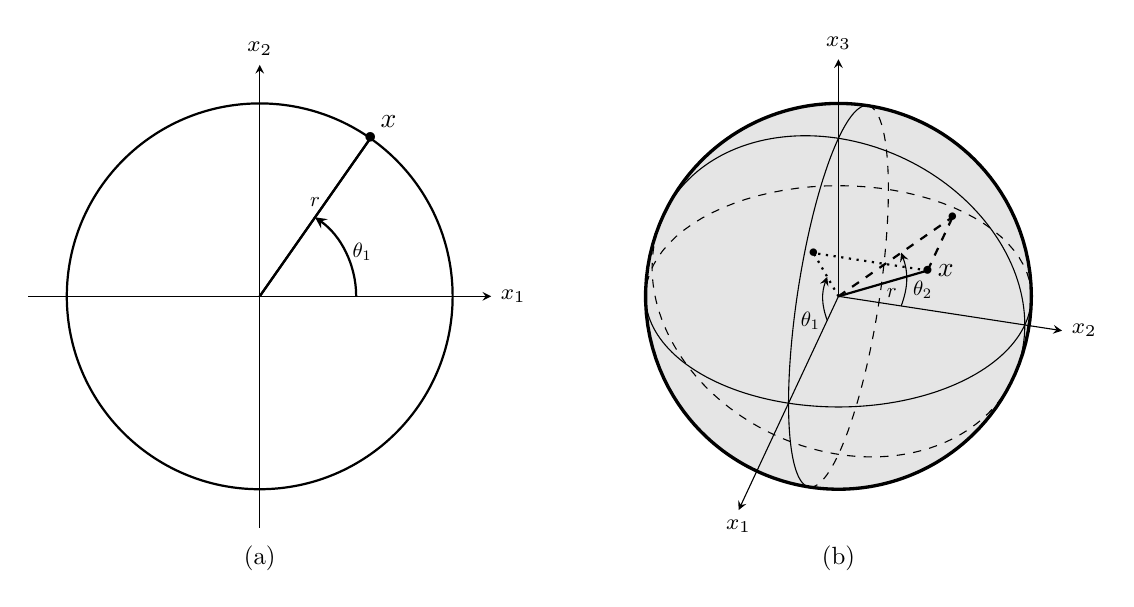
\begin{tikzpicture}[scale=.7]
\shorthandoff{>}

% CUIDADO
% Para el dibujo de la esfera, todo era hecho  en coordenadas esfericas de fisica (theta,phi)
% Para el punto x, se usan las coordenadas como en el libro, (theta_1,theta_2)
% (on dos parametrizaciones de la misma cosa...)
%
% Proyeccion para diburar un punto (x_1,x_2,x_3) teniendo en cuenta el angulo de vision
\pgfmathdeclarefunction{projx}{2}{\pgfmathparse{#1*cos(\Az)-#2*sin(\Az)}}
\pgfmathdeclarefunction{projy}{3}{\pgfmathparse{#1*sin(\Az)*sin(\El)+#2*cos(\Az)*sin(\El)+#3*cos(\El)}}


% unas definiciones para elegir el angolu de vision
\pgfmathsetmacro{\El}{35} % Elevacion
\pgfmathsetmacro{\Az}{-105}% Azimuth
%
\pgfmathsetmacro\r{3.5} % radio del circulo (d=2) y de la esfera (d=3)
%
%
% punto x para el caso d = 2
\pgfmathsetmacro\tpbi{55} % theta_1
\pgfmathsetmacro\xpbi{\r*cos(\tpbi)} % x_1
\pgfmathsetmacro\ypbi{\r*sin(\tpbi)} % x_2
%
%
% punto x para el caso d = 3
\pgfmathsetmacro\tu{60} % theta_1 punto x
\pgfmathsetmacro\td{45} %theta_2 punto x
\pgfmathsetmacro\xp{\r*cos(\tu)} % x_1 de x
\pgfmathsetmacro\yp{\r*sin(\tu)*cos(\td)} % x_2 de x
\pgfmathsetmacro\zp{\r*sin(\tu)*sin(\td)} % x_3 de x
%\pgfmathsetmacro\xp{\rp*cos(\tp)*cos(\pp)} % x_1 de x
%\pgfmathsetmacro\yp{\rp*sin(\tp)*cos(\pp)} % x_2 de x
%\pgfmathsetmacro\zp{\rp*sin(\pp)} % x_3 de x
%
%
% funcion permitiendo calcular phi(theta) dando la linea de cumbre
\pgfmathdeclarefunction{phicr}{1}{\pgfmathparse{
atan((sin(#1)*cos(\Az)+cos(#1)*sin(\Az))/(tan(\El)))
}}
%
% ====================================================================
%
% -----------------
% | Circulo d = 2 |
% -----------------
%
\begin{scope}
%
%  axes
% ------
%
\draw[>=stealth, ->] ({-1.2*\r},0)--({1.2*\r},0) node[right] {\footnotesize $x_1$};
\draw[>=stealth, ->] (0,{-1.2*\r})--(0,{1.2*\r}) node[above] {\footnotesize $x_2$};
%
%
%  Circulo
% --------
%
\draw[thick] (0,0) circle (\r);
%
%\draw (\r,0) node[below]{$r$};
%
%
%  punto x, r, theta_1
% --------------------
%
\draw[thick] (0,0) -- (\xpbi,\ypbi) node[scale=.9]{$\bullet$};
\draw[thick] (0,0) -- (\xpbi,\ypbi) node[above right]{$\boldsymbol{x}$};
\draw ({\xpbi/2},{1.05*\ypbi/2}) node[above,scale=.75]{$\boldsymbol{r}$};
\draw[->,>=stealth,thick] ({\r/2},0)  arc (0:\tpbi:{\r/2});
\draw ({\r*cos(\tpbi/2)/2},{\r*sin(\tpbi/2)/2}) node[right,scale=.75] {$\boldsymbol{\theta_1}$};
%
\node at (0,{-\r-1.25}) [scale=.9]{(a)};
\end{scope}
%
%
% ====================================================================
%
% ----------
% | Esfera |
% ----------
%
\begin{scope}[xshift=10.5cm]
%
%
%  angulo de visibilidad
% -----------------------
%
\pgfmathsetmacro\tv{-\Az}
%
%
% Axes
% -----
%
\draw[>=stealth, ->] (0,0)--({projx(\r*2,0)},{projy(\r*2,0,0)}) node[below]
{\footnotesize $x_1$};
\draw[>=stealth, ->] (0,0)--({projx(0,\r*1.2)},{projy(0,\r*1.2,0)}) node[right]
{\footnotesize $x_2$};
\draw[>=stealth, ->] (0,0)--(0,{projy(0,0,\r*1.5)}) node[above]
{\footnotesize $x_3$};
%
%
% Esfera
% ------
%
% interior de la esfera / linea de cumbre
\filldraw[very thick, domain=-\Az:-\Az+360, variable=\t, samples=180, fill opacity=.1]
plot ({projx(\r*cos(\t)*cos(phicr(\t)),\r*sin(\t)*cos(phicr(\t)))} , 
      {projy(\r*cos(\t)*cos(phicr(\t)),\r*sin(\t)*cos(phicr(\t)),\r*sin(phicr(\t)))});
%
% Ecuador (para visualisar la esfera), dado por phi = 0:
% parte visible
\draw[domain=-\Az+180:-\Az+360, variable=\t, samples=90]
plot ({projx(\r*cos(\t),\r*sin(\t))},{projy(\r*cos(\t),\r*sin(\t),0)});
%
% partie invisible
\draw[dashed, domain=-\Az:-\Az+180, variable=\t, samples=45]
plot ({projx(\r*cos(\t),\r*sin(\t))},{projy(\r*cos(\t),\r*sin(\t),0)});
%
% Linea de longitud para que se vea bien la surfaza: theta = 0 y 90
% parte visible theta = 0
\draw[domain=phicr(0):phicr(0)+180, variable=\p, samples=90]
plot ({projx(\r*cos(\p),0)},{projy(\r*cos(\p),0,\r*sin(\p))});
%
% partie escondida theta = 0
\draw[dashed, domain=phicr(0)+180:phicr(0)+360, variable=\p, samples=90]
plot ({projx(\r*cos(\p),0)},{projy(\r*cos(\p),0,\r*sin(\p))});
%
% parte visible theta = 90
\draw[domain=phicr(90):phicr(90)+180, variable=\p, samples=90]
plot ({projx(0,\r*cos(\p))},{projy(0,\r*cos(\p),\r*sin(\p))});
%
% partie escondida theta = 90
\draw[dashed, domain=phicr(90)+180:phicr(90)+360, variable=\p, samples=90]
plot ({projx(0,\r*cos(\p))},{projy(0,\r*cos(\p),\r*sin(\p))});
%
%
% Punto
% ------
%
%
% Posicion del punto x
\draw[thick] (0,0) --
({projx(\xp,\yp},{projy(\xp,\yp,\zp)})
node[scale=.75]{$\bullet$};
%
\draw[thick]
({projx(\xp,\yp},{projy(\xp,\yp,\zp)})
node[right]{$\boldsymbol{x}$};
%
%
% proyecciones para poner los angulos
% x1 = 0
%\draw[thick,dashed] ({projx(\xp,\yp},{projy(\xp,\yp,\zp})--({projx(0,\yp},{projy(0,\yp,\zp});
%\draw[thick,dashed] (0,0)--({projx(0,\yp},{projy(0,\yp,\zp});
%\draw[thick,dashed] ({projx(0,\yp},{projy(0,\yp,0})--({projx(0,\yp},{projy(0,\yp,\zp});
%
%
% notacion del radio
\pgfmathsetmacro{\propr}{.6} % distancia del radio para anotar "r"
\draw ({projx(\propr*\xp,\propr*\yp},{projy(\propr*\xp,\propr*\yp,\propr*\zp})
node[below,scale=.75] {$\boldsymbol{r}$};
%
%
% notacion del angulo theta_1
\pgfmathsetmacro{\proptu}{.45} % "radio" para dibujar el angulo
\draw[thick,dotted] ({projx(\xp,\yp},{projy(\xp,\yp,\zp})--({projx(\xp,0},{projy(\xp,0,\zp});;% proy x2=0
\draw[thick,dotted] (0,0)--({projx(\xp,0},{projy(\xp,0,\zp}) node[scale=.7]{$\bullet$};% proy x2=0
\draw[->,>=stealth]
({projx(\proptu*\xp,0)},{projy(\proptu*\xp,0,0)}) to [bend left=20]
node[pos=0,left,scale=.75] {$\boldsymbol{\theta_1}$}
({projx(\proptu*\xp,0)},{projy(\proptu*\xp,0,\proptu*\zp)});
%
%
% notacion del angulo theta_2
\pgfmathsetmacro{\propp}{.55} % "radio" para dibujar el angulo
\draw[thick,dashed] ({projx(\xp,\yp},{projy(\xp,\yp,\zp})--({projx(0,\yp},{projy(0,\yp,\zp});;% proy x1=0
\draw[thick,dashed] (0,0)--({projx(0,\yp},{projy(0,\yp,\zp}) node[scale=.7]{$\bullet$};% proy x1=0
\draw[->,>=stealth]
({projx(0,\propp*\yp)},{projy(0,\propp*\yp,0)}) to [bend right=20]
node[pos=0.3,right,scale=.75] {$\boldsymbol{\theta_2}$}
({projx(0,\propp*\yp)},{projy(0,\propp*\yp,\propp*\zp)});
%
\node at (0,{-\r-1.25}) [scale=.9]{(b)};
\end{scope}
%
\end{tikzpicture}
 \end{center}
% 
\leyenda{Coordenadas hiperesf\'ericas para un  punto dado de $\Rset^d$. (a) caso
  $d = 2$ y (b) caso $d = 3$.}
%
\label{Fig:MP:CoordenadasHiperesfericas}
\end{figure}

En el  caso de vector  a simetr\'ia  esf\'erica, aparece que  el rayo $R$  y los
angulos     son     independientes      y     se     puede     calcular     cada
distribuci\'on~\cite{FanKot90, And03, Lor54, Zoz12}:
%
\begin{teorema}
  Sea  \  $X  \sim  \ED(0,I,d_X)$  \  y \  su  representaci\'on  en  coordenadas
  hiperesf\'ericas \  $X_i = R \left( \prod_{k=1}^{i-1}  \sin\Theta_k \right) \cos
  \Theta_i, \quad 1 \le  i \le d$. Entonces $R$ y los $\Theta_i,  \: 1 \le i \le
  d-1$ \ son independientes y
  %
  \[
  p_R(r) = \frac{2  \pi^{\frac{d}{2}}}{\Gamma\left( \frac{d}{2} \right)} r^{d-1}
  d_X\left( r^2 \right)
  \]
  %
  \[
  p_{\Theta_i}(\theta_i)        =       \frac{\Gamma\left(       \frac{d-j+1}{2}
    \right)}{\sqrt{\pi}   \,  \Gamma\left(   \frac{d-j}{2}  \right)}   \,  \big(
  \sin\theta_i \big)^{d-i-1}  \, \un_{[0 \;  \pi)}(\theta_i), \quad 1 \le  i \le
  d-2 , \qquad p_{\Theta_{d-1}}(\theta_{d-1}) =  \frac{1}{2 \pi} \, \un_{[0 \; 2
    \pi)}(\theta_{d-1})
  \]
  %
\end{teorema}
%
\begin{proof}
  Sea      la       transformaci\'on      $g:      (x_1,\ldots,x_d)      \mapsto
  (r,\theta_1,\ldots,\theta_{d-1})$. La Jacobiana de $g^{-1}$ tiene la forma
  %
  \[
  \Jac_{g^{-1}} = \begin{bmatrix}
  %
    \frac{\partial x_1}{\partial r} & \frac{\partial x_1}{\partial \theta_1} & 0 & \cdots & 0\\
  %
    \vdots & \vdots & \ddots & \ddots & \vdots\\
  %
    \vdots & \vdots &  & \ddots  & 0\\
  %
    \frac{\partial x_{d-1}}{\partial r} & \frac{\partial x_{d-1}}{\partial
    \theta_1} & \cdots & & \frac{\partial x_{d-1}}{\partial \theta_{d-1}}\\
  %
    \frac{\partial x_d}{\partial  r} & \frac{\partial  x_d}{\partial \theta_1} &
    \cdots & \cdots & \frac{\partial x_d}{\partial \theta_{d-1}}
  %
  \end{bmatrix}
  \]
  %
  Desarrolando   el   determinante  por   la   \'ultima   columna  por   ejemplo
  (ver~\cite{Bha97, HorJoh13}), y as\'i por inducci\'on se obtiene
  %
  \[
  \left|   \Jac_{g^{-1}}  \right|  =   r^{d-1}  \prod_{j=1}^{d-2}   \left(  \sin
    \theta_i\right)^{d-j-1}
  \]
  %
  Entonces,  por  transformaci\'on  (ver  secci\'on~\ref{Sec:MP:Transformacion})
  tenemos
  %
  \[
  f_{R,\Theta_1,\ldots,\Theta_{d-1}}(r,\theta_1,\ldots,\theta_{d-1}) = d_X\left(
    r^2    \right)     r^{d-1}    \prod_{j=1}^{d-2}    \left(     \left(    \sin
      \theta_i\right)^{d-j-1} \un_{[0 \; \pi)}(\theta_i) \right) \, \un_{[0 \; 2
    \pi)}(\theta_{d-1})
  \]
  %
  Claramente  se  factoriza  probando  la  independencia  y  la  forma  de  cada
  distribuci\'on   marginal.    El   factor   viene    de   la   normalizaci\'on
  (ver~\cite[Ec.~8.380-2]{GraRyz15}   para  los   angulos,   lo  que   determina
  necesariamente el del rayo).
\end{proof}
%
Obviamente,  se  recupera la  ley  de  \ $R  \egald  \|X\|$  \ que  encontramos.
Ad\'emas, estas  coordenadas hiperesf\'ericas, a $r=1$,  parametriza $\Sset_d$ y
permite por ejemplo de probar la independencia entre $\|X\|$ y $\frac{X}{\|X\|}$
(y entonces la escritura en mezcla), de calcular directamente \ $\Phi_U(\omega)$
\ para \ $U \sim \U(\Sset_d)$,  o de vincular las generadoras caracter\'istica y
de densidad entre otros.

En la familia el\'iptica, hay una subfamilia particular que queda invariante por
marginalizaci\'on, y extensi\'on, como la gaussiana por ejemplo:
%
\begin{definicion}[Consistencia~\cite{Yao73, Kan94}]
%
  Sea \  $X = \begin{bmatrix} X_1 &  \cdots & X_d \end{bmatrix}$  \ a simetr\'ia
  el\'iptica  de  generadora de  densidad  $d_X$.   Este  vector es  dicho  {\em
    consistente}   si  la   generadora  de   densidad  \   $d_{X'}$  \   de  $X'
  = \begin{bmatrix} X_1 & \cdots &  X_{d'} \end{bmatrix}$ \ tiene la misma forma
  que \ $d_X$  \ donde el par\'ametro  dimensional \ $d$ \ es  reemplazado por \
  $d'$.  En  otros t\'erminos tenemos  invarianza por marginalizaci\'on si  $d' <
  d$, pero se puede ver $X$ como marginal de un vector m\'as grande con la misma
  generadora de probabilidad re-emplazando $d$ por $d'$.

  Se prueba que, equivalentemente,  la generadora caracter\'istica \ $\varphi_X$
  \  no es  relacionada a  \ $d$  (ver~\cite{Kan94, FanKot90}  para  la prueba).
  Entonces, $\varphi_X$  va a ser  una generadora caracter\'istica de  un vector
  aleatorio   de  cualquiera   dimensi\'on  \   $d  \in   \Nset_0$,  o,   con  la
  caracterisaci\'on por functiones definida no negativa (ver teorema de Bocher),
  \  $\varphi_X  \in  \PDSI$  (ver   notaciones,  y  las  a  continuaci\'on  del
  teorema~\ref{Teo:MP:GeneradorasCaracteristicas}).
\end{definicion}


Si \  $X$ \ a simetr\'a  esf\'erica (y por transformaci\'on  af\'in a simetr\'ia
el\'iptica)  se escribe siempre  como mezcla  de escala  de base  uniforme, esta
escritura estoc\'astica  no es \'unica. Por  ejemplo, si consideramos $X  = A \,
G$, con \ $A$ \ variable aleatoria positiva \ y \ $G \sim \N(0,I)$ independiente
de $G$,  queda claro  que \ $X$  \ es  a simetr\'ia esf\'erica.  Estos vectores,
llamados {\em mezcla de escala de  base gaussiana}, o simplemente {\em mezcla de
  escala  gaussiana}  (GSM  para  gaussian  scale mixture  en  ingl\'es)  fueron
estudiados  intensivamente de  manera formal~\cite{Kan94,  Yao73,  Ver64, Pic70,
  Kel71,  Kin72, KeiSte74,  Tei60, AndMal74}.   Ecuentra aplicaciones  en varias
area, modelizando la  textura de imagenes o datos de  radar (ej.  suma aleatoria
de  vectores gaussianos)~\cite{PorStr03,  BomBea08,  Sel08, ShiSel07,  ZozVig10,
  TisNic04, TodTab07}.

Una  pregunta natural  es  de saber  si  se puede  escribir  cualquier vector  a
simetr\'ia esf\'erica como mezcla de  escala de base gaussiana.  La respuesta es
negativa. Por ejemplo,  del dominio de definici\'on de  la variable, queda claro
que un  vector uniforme sobre la  esfera no puede  ser mezcla de escala  de base
gaussiana (ver un otro  contra-ejemplo en~\cite{Pic70}).  Escribir un vecor como
tal  mezcla es posible  solamente bajo  restricciones.  M\'as  precisamente, una
condici\'on necesaria y suficiente es que la variable debe ser consistente, como
lo           prob\'o           Sch{\oe}nberg~\cite[Teo.~2]{Sch38}           (ver
tambi\'en~\cite[Teo.~2]{SteVan05},            \cite[Lem.~2.2]{Yao73}           o
\cite[Teo.~1]{Kan94}).
%
\begin{teorema}[Sch{\oe}nberg'38 -- a partir de la generadora caracter\'istica]
\label{Teo:MP:SchoenbergCaracteristica}
%
Sea \ $X  \sim \ED\left( m ,  \Sigma , \varphi_X \right)$.  Entonces  $X$ es una
mezcla de gaussiana si y solamente si $X$ es consistente, es decir
  %
  \[
  X \,  \egald \,  A \, \Sigma^{\frac12}  \, G  + m \quad  \Leftrightarrow \quad
  \varphi_X \in \PDSI
  \]
  %
  con \ $A > 0$ \ independiente de \ $G \sim \N(0,I)$.
\end{teorema}
%
\begin{proof}
  La directa es inmediata de la f\'ormula de esperanza total
  %
  \[
  \varphi_X(w)  = \Esp\big[  \, \Esp\left[  \varphi_G\left( A  w  \right) \left.
    \right| A\right] \, \big]
  \]
  %
  conjuntamente a \ $\varphi_G: w \mapsto e^{-\frac{w}{2}} \: \in \PDSI$.

  La rec\'iproca es m\'as dificil a probar. Para los detalles, dejamos el lector
  a~\cite{Sch38}. Los  elementos de prueba  son los siguientes. De  la escritura
  como mezcla de escala uniforme tenemos entonces para cualquier \ $d$
  %
  \[
  \varphi_X\left(  w^2  \right)  =  2^{\frac{d}{2}-1}  \Gamma\left(  \frac{d}{2}
  \right) \int_{\Rset_+} \left(  w r \right)^{1-\frac{d}{2}} J_{\frac{d}{2}-1}(w
  r) \, dP_{R_d}(r)
  \]
  %
  con \  $R_d$ \ la  variable generadora de  base uniforme correspondiente  a la
  dimension   $d$   (ver   prueba  del   teorema~\ref{Teo:MP:MezclaUniforme}   y
  ejemplo~\ref{Ej:MP:GeneCaracUniformeEsfera}).  Por   cambio  de  variables  se
  escribe tambi\'en
  %
  \[
  \varphi_X\left(  w^2 \right)  = \int_{\Rset_+}  2^{\frac{d}{2}-1} \Gamma\left(
    \frac{d}{2}   \right)   \left(    w   r   \sqrt{d}   \right)^{1-\frac{d}{2}}
  J_{\frac{d}{2}-1}\left(  w r  \sqrt{d}  \right) \,  dP_{R_d}\left( r  \sqrt{d}
  \right)
  \]
  %
  Eso siendo valid para cualquier orden,  se nota $P_R$ el l\'imite de $P_{R_d}$
  cuando $d$ tiende al infinito.  Luego,  el desarollo de Taylor de la funci\'on
  de Bessel y de  la f\'ormula de Stirling~\cite[Ec.~8.402~y~8.327]{GraRyz15} se
  prueba que
  %
  \[
  \lim_{d \to +\infty} 2^{\frac{d}{2}-1} \Gamma\left( \frac{d}{2} \right) \left(
    w  r \sqrt{d} \right)^{1-\frac{d}{2}}  J_{\frac{d}{2}-1}\left( w  r \sqrt{d}
  \right) \: = \: e^{-\frac{w^2 r^2}{2}}
  \]
  %
  Todo el  juego consiste a probar  que la convergencia es  uniforme, para poder
  intercambiar   l\'imite   e    integral.    Dio   una   prueba   Sch{\oe}nberg
  en~\cite{Sch38},  y  luego propuso  una  ``m\'as  moderna''  Steerneman y  van
  Perlo-ten-Kleij  en~\cite{SteVan05}.  Basicamente  se reconoce  en  $w \mapsto
  2^{\frac{d}{2}-1}   \Gamma\left(  \frac{d}{2}   \right)   \left(  w   \sqrt{d}
  \right)^{1-\frac{d}{2}}   J_{\frac{d}{2}-1}\left(  w   \sqrt{d}   \right)$  la
  funci\'on  caracter\'istica  de  $q_d(x)  \propto  \left(  1  -  \frac{x^2}{d}
  \right)_+^{\frac{d-3}{2}}$  \  que tiende  a  la  gaussiana  (ver por  ejemplo
  secci\'on~\ref{Sssec:MP:StudentR}).   Se usa el  lema de  Scheff\'e o  de Riez
  (ver~\cite{Rie28,  Sch47, Nov72,  Kus10} o  \cite{AthLah06,  Bog07:v1, Bil12})
  para probar la convergencia de la integral.
% (es similar al uso del teorema de convergencia dominada).
\end{proof}
%
\noindent  Se  encuentra  una  prueba alternativa  tambi\'en  en~\cite{FanKot90,
  Kin72}.

Este  teorema pone  en  juega la  condici\'on  necesaria y  suficiente sobre  la
funci\'on caracter\'istica para tener una  mezcla de escala gaussiana, as\'i que
no es necesario que \ $X$ \ admita una densidad de probabilidad. Sin embargo, al
imagen de la  consistencia que se exprime tambi\'en a  trav\'es de la generadora
de  densidad,  el teorema  de  Sch{\oe}nberg  tiene  una versi\'on  usando  esta
generadora.   Por  eso,  introducimos  el conjunto  de  funciones  complatemente
monotonas   sobre  $\Rset_+$   hasta   un  cierto   orden,   y  para   cualquier
orden~\footnote{Una funci\'on  \ $f: I \subset  \Rset \mapsto \Rset$  \ es dicha
  {\em absolutamente monotona} si es continua, diferenciable a todos los ordenes
  en el interior de $I$, y todas sus derivadas son positivas, $ \forall \: k \in
  \Nset, \quad f^{(k)} \ge 0$.  $f$ \ es dicha {\em completamente monotona} si \
  $f(-x)$ \ es absolutamente monotona~\cite{Ber29}.} (ver notaciones):
%
\[
\CM_n = \left\{ f \in C^{n-1}(\Rset_+) \tq \forall \, k = 0 , \ldots , n-1, \:\:
  (-1)^k  f^{(k)}  \ge 0  \:  \et \:(-1)^{n-1}  f^{(n-1)}  \:  \mbox{ es  decreciente}
\right\}
\]
%
y
%
\[
\CM = \bigcap_{n=0}^{+\infty} \CM_n =  \left\{ f \in
  C^{\infty}(\Rset_+)  \tq \forall \,  k \in  \Nset, \:\:  (-1)^k f^{(k)}  \ge 0
\right\}
\]
%
\begin{teorema}[Sch{\oe}nberg'38 -- a partir de la generadora de densidad]
\label{Teo:MP:SchoenbergDensidad}
%
  Sea \ $X \sim \ED\left( m , \Sigma , d_X \right)$.  Entonces $X$ es una mezcla
  de gaussiana si y solamente si $d_X$ es completamente monotona sobre $\Rset_+$
  %
  \[
  X \, \egald \, A \, \Sigma^{\frac12}  \, G + m \quad \Leftrightarrow \quad d_X
  \in \CM
  \]
  %
  con \ $A > 0$ \ independiente de \ $G \sim \N(0,I)$.
\end{teorema}
%
\begin{proof}
  La prueba se  apoya sobre el teorema de  Haussdorf-Bernstein-Widder que prueba
  la equivalencia  entre la clase de  funciones completamente monotonas  y la de
  las   funciones  \  $f$   \  que   se  escriben   como  una   transformada  de
  Laplace-Stieltjes~\footnote{Por     definici\'on,    la     transformada    de
    Laplace-Stieltjes de una medida \ $\mu$  \ definida sobre $\Rset_+$ \ es una
    funci\'on   de  un   n\'umero  complejo   \  $\displaystyle   \LS[\mu](s)  =
    \int_{\Rset_+} e^{-s t}  \, d\mu(t)$. Se prueba que existe  un real \ $x_0$,
    llamado abscisa  de convergencia tal que  la convergencia es  uniforma en el
    semi-plano \ $\real{s}  > x_0$, y a continuaci\'on  tal que \ $\displaystyle
    \LS[\mu]$ \  es anal\'itica en este  semi-plano.  Si \  $\displaystyle \mu =
    \sum_i  \alpha_i  \delta_{t_i}$  \  es  una medida  discreta  se  obtiene  \
    $\displaystyle  \LS[\mu](s) = \sum_i  \alpha_i e^{-s  t_i}$ \  conocido como
    serie de Dirichlet, y si \ $\mu$ \ admite una densidad \ $g$, $\displaystyle
    \LS[\mu](s) \equiv  \L[g](s) = \int_{\Rset_+} e^{-s  t} \, g(t) \,  dt$ \ es
    dicha transformada de Laplace ordinaria de  \ $g$.  Para $s = \imath \omega$
    \ con  $\omega \in  \Rset$, las transformaciones  de Laplace-Stieltjes  y de
    Laplace coinciden con las transformaciones $\FS$ de Fourier-Stieltjes y $\F$
    de           Fourier            ordinaria           (ver           tambi\'en
    secci\'on~\ref{Ssec:MP:FuncionCaracterisica} para esta transformaci\'on). Al
    imagen  de   la  transformada  de  Fourier  inversa   que  vimos  brevemente
    secci\'on~\ref{Ssec:MP:FuncionCaracteristica},    existen    f\'ormulas   de
    inversi\'on  de   las  transformadas  de  Laplace-Stieltjes   y  de  Laplace
    ordinaria, denotadas  \ $\LS^{-1}$  \ y \  $\L^{-1}$ \  respectivamente.  Se
    referir\'a     por    ejemplo     a~\cite{Wid46}     para    tener     m\'as
    detalles. \label{Foot:MP:LaplaceStieltjes}} (en el eje real)
  %
  \[
  f(t) = \int_{\Rset_+} e^{-t u} d\mu(u)
  \]
  %
  donde  $\mu$  es  una  medida finita  (ver~\cite[Teo.~3]{Sch38},  \cite{Ber29,
    Hau21:I, Hau21:II,  Wid31}, \cite[\S~12]{Wid46}, \cite[\S~XIII.4]{Fel71}).
  %
  % Feller v2, p.  439; Widder p. 160; Schoenberg th. 3  y sec. 4 (Hausdorff'21,
  % Bernstein'29, Carlson'21),
  % 
  Con el  cambio de variables  $u = \frac{1}{2  a^2}$ \ y  \ $\mu\big( (0  \; u)
  \big) =  (2 u)^{\frac{d}{2}} P_A\left( \left( \frac{1}{\sqrt{2  u}} \; +\infty
    \right) \right)$, se aplica entonces este teorema a (f\'ormula de probabilidad
  total)
  %
  \[
  d_X(r)  =  (2 \pi)^{-\frac{d}{2}} \int_{\Rset_+} a^{-d} e^{-\frac{r}{2 a^2}} dP_A(a) 
  \]

  Basicamente la  directa viene  de esta  f\'ormula de probabilidad  total y  de \
  $\displaystyle     \frac{d^k    e^{-\frac{r}{2    a^2}}}{dr^k}     =    (-1)^k
  \frac{e^{-\frac{r}{2 a^2}}}{2^k  a^{2 k}}$ \  (se usa para  poder intercambiar
  derivada    e     integral    el    teorema     de    convergencia    dominada
  sec.~\ref{Ssec:MP:VAPreliminaria}).

  De  nuevo,  la  rec\'iproca  es  m\'as  d\'ificil  a  probar  y  es  detallada
  en~\cite[\S~12]{Wid46} por ejemplo.  Basicamente, se  muestra que si \ $d_X$ \
  es  completamente  monotona,  se  puede  escribir \  $\displaystyle  d_X(n)  =
  \int_{\Rset_+}  v^n  d\mu(v)  =  \int_{\Rset_+}  e^{-n  u}  d\mu\left(  e^{-u}
  \right)$, momento de  orden \ $n$ con respecto a una  medida de probabilidad \
  $\mu$~\cite{Hau21:I, Hau21:II},  visto como transformada  de Laplace-Stieltjes
  en \ $t  = n$.  Se define la funci\'on \  $\displaystyle f(r) = \int_{\Rset_+}
  e^{- r  u} d\mu\left( e^{-u}  \right)$ \  que coincide con  \ $d_X$ \  sobre \
  $\Nset$.   Se  prueba  finalmente  que   \  $d_X(r)  -  f(r)$  \  se  extiende
  analiticamente  en el  semi  plano  complejo \  $\real{s}  \ge 0$  \  y de  la
  analiticidad  que  \ $d_X$  \  y  \ $f$  \  coinciden  entonces  en todo  este
  semi-plano~\cite{Car21, CarKro05}.
\end{proof}

Se  notar\'a  que  la consistencia  se  manifesta  tambi\'en  a trav\'es  de  la
generadora de la mezcla gaussiana:
%
\begin{lema}\label{Lem:MP:AIndependienteD}
  Sea  \ $\varphi_X  \in  \PDSI$ (o  $d_X  \in \CM$).  Entonces, para  cualquiera
  dimension \ $d$ \ y  $X \sim \ED(m,\Sigma,\varphi_X)$ \ $d$-dimensional, en la
  escritura  \ $X  \egald  A \,  \Sigma^{\frac12} G  +  m$ \  con  \ $A  > 0$  \
  independiente de \ $G  \sim \N(0,I)$ la ley de $A$ no  depende de la dimension
  $d$.
\end{lema}
%
\begin{proof}
  La  prueba  es  inmediata  del   hecho  que,  para  cualquiera  matriz  $M  \in
  \Mat_{d,n}(\Rset)$ de rango lleno con $d  \le n$, \ $X \egald A \Sigma^{\frac12}
  G $ \ con  \ $G \sim \N(0,I)$ \ $n$-dimensional, tenemos $X' =  M X \egald A M
  \Sigma^{\frac12} G \egald A \left( M  \Sigma M^t \right)^{\frac12} G'$ \ con \
  $G'         \sim        \N(0,I)$         \         $d$-dimensional        (ver
  teorema~\ref{Teo:MP:StabilidadGaussiana}).  Una   mezcla  de  gaussiana  queda
  mezcla por proyecci\'on,  con la misma generadora $A$, y  al rev\'es puede ser
  vista como  proyecci\'on de una  mezcla de dimensi\'on  m\'as grande (no  va a
  cambiar la generadora)~\footnote{Cuidense  de que no anda si  salimos a partir
    de una mezcla de base uniforme: como lo vamos a ver, las proyecciones no son
    uniforme m\'as si $d  < n$, lo que se intuite por  razones de dominio imagen
    (bolas por proyecci\'on de la esfera).}.
\end{proof}

Si  en  la  escritura  como  mezcla  de  escala  de  base  uniforme  se  escribe
sencillamente  la  ley  del rayo  \  $R$,  se  puede tambi\'en  caracterizar  la
generadora en  el caso de mezcla de  base gaussiana. Viene de  la escritura como
mezcla, donde  se reconoce  une transformada de  Laplace-Stieltjes (ver  nota de
pie~\ref{Foot:MP:LaplaceStieltjes}).

\begin{lema}\label{Lem:MP:PaLaplaceInversa}
  Sea \ $X \sim \ED(m,\Sigma,\varphi_X)$ \ mezcla de escala gaussiana, con \ $A$
  la  variable aleatoria  generadora.  $\varphi_X$  \ admite  una continuaci\'on
  anal\'itica \ $s \mapsto \varphi_X(s)$ \ en el semi-plano complejo \ $\real{s}
  > 0$.  Notando \ $\LS$ \ la transformada de Laplace-Stieltjes y \ $\LS^{-1}$ \
  la transformada  inversa (ver nota  de pie~\ref{Foot:MP:LaplaceStieltjes}), la
  funci\'on de repartici\'on de \ $A$ \ es dada por
  %
  \[
  F_A(a) = \LS^{-1}[\varphi_X] \left( \left( 0 \; \frac{a^2}{2} \right) \right)
  \]
  %
  Si la medida \ $P_A$ \ admite una densidad \ $p_A$, se obtiene inmediatamente
  %
  \[
  p_A(a) = a \, \L^{-1}[\varphi_X] \left(\frac{a^2}{2} \right)
  \]

  Similarmente, si \ $X$ \ admite una  generadora de densidad \ $d_X$, \ $d_X$ \
  se extiende tambi\'en anal\'iticamente en el semi-plano complejo \ $\real{s} >
  0$ \ y se obtiene
  %
  \[
  \int_0^a u^{-d} dP_A(u) = (2 \pi)^{\frac{d}{2}} \, \LS^{-1}[d_X] \left( \left(
      \frac{1}{2 a^2} \; +\infty \right) \right) \qquad \mbox{y} \qquad f_A(a) =
  (2 \pi)^{\frac{d}{2}} \, a^{d-3} \, \L^{-1}[d_X]\left( \frac{1}{2 a^2} \right)
  \]
  %
  respectivamente.
\end{lema}
%
\begin{proof}
  Para \ $U$ \ uniforme sobre la  esfera, del desarollo en serie de la funci\'on
  de   Bessel~\cite[Ec.~8.402]{GraRyz15},  es  claro   que  \   $\varphi_U(w)  =
  2^{\frac{d}{2}-1}  \Gamma\left(   \frac{d}{2}  \right)  \,  w^{-\frac{d-2}{4}}
  J_{\frac{d}{2}-1}(\sqrt{w})$  \ admite  una continuaci\'on  anal\'itica  en el
  semi-plano  complejo $\real{s}  >  0$.   De la  mezcla  uniforme, tambi\'en  \
  $\displaystyle \varphi_X(w) = \int_{\Rset_+} \varphi_X(r w) \, dP_R(r)$ admite
  una  continuaci\'on   anal\'itica  en  el  semi-plano   complejo  $\real{s}  >
  0$. Luego, de la escritura de mezcla gaussiana tenemos
  %
  \[
  \varphi_X(w) = \int_{\Rset_+} e^{-\frac{w a^2}{2}} \, dP_A(a) = \int_{\Rset_+}
  e^{- w t} \, dP_A(\sqrt{2 t})
  \]
  %
  por cambio  de variables. Se  reconoce la transformada de  Laplace-Stieltjes \
  $\L$ \ de la medida \ $\mu$  \ (definida sobre $\Rset_+$) dada por \ $\mu\big(
  (0  \;  t)  \big) =  P_A\left(  \left(  0  \;  \sqrt{2  t} \right)  \right)  =
  F_A(\sqrt{2  t})$.  La  funci\'on  de repartici\'on  en  \ $\sqrt{2  t}$ \  es
  entonces dada por la transformada  inversa de Laplace-Stieljes de \ $s \mapsto
  \varphi_X(s)$, lo  que cierra  la prueba para  \ $F_A$.  Ahora,  para escribir
  $p_A$ \ se puede diferenciar $F_A$ obtenido, o simplemente escribir $dP_A(a) =
  p_A(a) \, da$, \ie \ $dP_A(\sqrt{2 t}) = \frac{p_A(\sqrt{2 t})}{\sqrt{2 t}} \,
  dt$ \ y reconocer en \  $\varphi(s)$ \ la transformada ordinaria de Laplace de
  $t \mapsto \frac{p_A(\sqrt{2 t})}{\sqrt{2 t}}$.

  La prueba que \ $d_X$ \  se extiende analiticamente en el semi-plano $\real{s}
  >0 $  es dada  en~\cite[Cap.~IV, Teo.~3a]{Wid46}~\footnote{Se prueba  de hecho
    que una  funci\'on absolutamente monotona sobre  $\Rset_-$, como lo  es \ $r
    \mapsto d_X(-r)$,  se extiende analiticamente  en el semi-plano  $\real{s} <
    0$.}. Basicamente, siendo  \ $d_X \in C^\infty$, se  escribe su desarollo de
  Taylor en torno a un $r_0 > 0$ y  se prueba que sobre $r \in (0 \; r_0)$, esta
  serie de t\'erminos todos  positivos converge uniformamente. Por consecuencia,
  se  tiene la  convergencia uniforme  tambi\'en para  \ $r  = s$  \ en  la bola
  compleja \ $|s-r_0|  < r_0$. Se cierra la prueba de  la validez para cualquier
  $r_0 > 0$. A continuaci\'on,  la forma de \ $P_A$ \ y \ $p_A$  \ a partir de \
  $d_X$ \ viene de los mismos pasos, saliendo de
  %
  \[
  d_X(r) =  \int_{\Rset_+} (2 \pi)^{-\frac{d}{2}} \,  a^{-d} e^{-\frac{r}{2}} \,
  dP_A(a) = (2 \pi)^{\frac{d}{2}}  \, \int_{\Rset_+} (2 t)^{\frac{d}{2}} \, e^{-
    w t} \, dP_A\left( (2 t)^{-\frac12} \right)
  \]
  %
  y introduciendo la medida \ $\mu_A$ \ definida por \ $\displaystyle \mu_A(B) =
  \int_B (2  t)^{\frac{d}{2}} \, dP_A\left(  (2 t)^{-\frac12} \right)$ \  por un
  lado, y escribiendo \ $dP_A(a) = p_A(a) da$ \ por el otro lado.
\end{proof}

Cuando se puede extender \ $\varphi_X$ \  o \ $d_X$ \ al eje complejo imaginario
puro, $w =  \imath \, \omega$ \ o \  $r = \imath \, \omega$  \ se reemplazan las
transformadas de Laplace-Stieltjes y Laplace ordinarias (y sus inversas) por las
de  Fourier-Stieltjes   \  $\FS$\   y  Fourier  ordinaria   \  $\F$  \   (y  sus
inversas)~\footnote{Se   puede  tambi\'en  pensar   a  la   transformaci\'on  de
  Mellin-Stieltjes   y  la   de  Mellin   ordinario  dada   respectivamente  por
  $\displaystyle  \MS[\mu](s) =  \int_{\Rset_+} t^s  \, d\mu(t)$  \quad  y \quad
  $\displaystyle  \M[g](s) = \int_{\Rset_+}  t^{s-1} \,  g(t) \,  dt$, definidas
  sobre una  franja del plano  complejo del tipo  \ $\real{s} \in (x_m  \; x_M)$
  (abscisas de convergencia), \  y usar sus propiedades remarcables~\cite{Zol57,
    Pou99, Pou10,  Wid46, ParKam01}.   En el caso  con densidad por  ejemplo, se
  reconoce en \  $g_X(r) = r^{d-1} d_X\left( r^2 \right)$ \  (ley del rayo, bajo
  un factor) lo  que se llama convoluci\'on af\'in, entre \  $g_G(r)$ \ (ley del
  rayo  de la  gaussiana)  \  y la  medida  de \  $A$,  $\displaystyle g_X(r)  =
  \int_{\Rset_+} \frac{1}{a} g_G\left( \frac{r}{a} \right) \, p_A(a) \, da$.  Al
  imagen de las  propiedades de la transformada de  Laplace, la transformaci\'on
  de Mellin de  una convoluci\'on af\'in es el  producto de las transformaciones
  de Mellin, y por un lado \ $\M[t^\alpha g(t)](s) = \M[g](s+\alpha)$ \ y por el
  otro lado  \ $\M[g(r^\alpha)](s) = |\alpha|^{-1}  \M[g](s/\alpha)$.  As\'i, se
  obtiene  sencillamente,  de  \  $\M[d_G](s)  =  2^s  \Gamma(s)$~\cite[Cap.~12,
  Tabla~12.1]{Pou10}   o~\cite[Cap.~18,  Tabla~18.1]{Pou99}   \   $\M[p_A](s)  =
  \frac{\pi^{\frac{d}{2}}              \M[d_X]\left(             \frac{s+d-1}{2}
    \right)}{2^{\frac{s-1}{2}} \Gamma\left( \frac{s+d-1}{2} \right)}$.
  % \ para \ $\real(s) > 1-d$.
  Similarmente,  se  muestra  en  el  caso  con densidad  que  \  $\M[p_A](s)  =
  \frac{\M[\varphi_X]\left(       \frac{1-s}{2}       \right)}{2^{\frac{1-s}{2}}
    \Gamma\left( \frac{1-s}{2} \right)}$,
  % \ para \ $\real{s} < 1$,
  \   y   \   obviamente   \  $\M[\varphi_X]   =   \frac{\pi^{\frac{d}{2}}   4^s
    \Gamma(s)}{\Gamma\left( \frac{d}{2} - s \right)} \M[d_X]\left( \frac{d}{2} -
    s \right)$  \ (lo  que se obtiene  tambi\'en a  partir de la  relaci\'on via
  transformada de  Hankel entre esta generadoras). Se  puede referirse tambi\'en
  a~\cite[\S~3.2.1]{Zoz12}).  }
%
\cite{Zol57, Pou99, Pou10, Wid46, ParKam01}.

\

Varios vectores  aleatorios que hemos visto  caen en la  familia el\'iptica.  No
admiten todas una  densidad con respecto a la medida de  Lebesgue, como lo hemos
visto con la ley  uniforme sobre la esfera (admite una con  respecto a la medida
de Haar),  tampoco no son  todas consistentes (y  entonces no se  escriben todas
como mezcla de escala de base gaussiana).
%
\begin{ejemplo}[Distribuci\'on gaussiana]
%
  Sea \ $X \sim \N(m,\Sigma)$.  Entonces, \ $X \sim \ED(m,\Sigma,\varphi_X)$ \ o
  equivalentemente \ $X \sim \ED(m,\Sigma,d_X)$ con
  %
  \[
  \varphi_X(u)   =  e^{-\frac{u}{2}}   \qquad  \mbox{y}   \qquad  d_X(r)   =  (2
  \pi)^{-\frac{d}{2}} e^{- \frac{r}{2}}
  \]
  
  Eso da la ley del rayo
  %
  \[
  p_R(r)  =  \frac{1}{2^{\frac{d}{2}-1}  \Gamma\left(  \frac{d}{2}  \right)}  \:
  r^{d-1} e^{- \frac{r^2}{2}}
  \]
  %
  Aparece   que  \   $R^2  \sim   \G\left(  \frac{d}{2}   ,   \frac12\right)$  \
  distribuci\'on gamma.
  
  Adem\'as,   la  generadora   caracter\'istica  siendo   independiente   de  la
  dimensi\'on \  $d$, \  $\Phi_X \in \PD$,  o equivalentemente la  generadora de
  densidad  \ $d_X$ \  teniendo la  forma que  damos para  cualquiera dimensi\'on
  (cambiar  de  dimensi\'on es  equivalente  a  cambiar  $d$), la  gaussiana  es
  consistente;  Las marginales  de  una gaussiana  son  gaussianas, y  cualquiera
  gaussiana puede ser vista como  marginal de gaussiana de cualquiera dimensi\'on
  m\'as grande.

  Obviamente, se  escribe como mezcla  de escala  de gaussiana con  \ $A =  1$ \
  variable cierta.
\end{ejemplo}

\begin{ejemplo}[Distribuci\'on Student-$t$]
%
  Sea \ $X \sim \T_\nu(m,\Sigma)$.  Entonces, \ $X \sim \ED(m,\Sigma,\varphi_X)$
  \ o equivalentemente \ $X \sim \ED(m,\Sigma,d_X)$ con
  %
  \[
  \varphi_X(u)   =  \frac{\nu^{\frac{\nu}{4}}}{2^{\frac{\nu}{2}-1}  \Gamma\left(
      \frac{\nu}{2}   \right)}   \,  u^{\frac{\nu}{4}}   K_{\frac{\nu}{2}}\left(
    \sqrt{\nu \,  u} \right) \qquad \mbox{y} \qquad  d_X(r) = \frac{\Gamma\left(
      \frac{d+\nu}{2}      \right)}{(\pi     \nu)^{\frac{d}{2}}     \Gamma\left(
      \frac{\nu}{2}    \right)}   \left(    1    +   \frac{r}{\nu}    \right)^{-
    \frac{d+\nu}{2}}
  \]

  Se obtiene de \ $d_X$ \ la ley de rayo
  %
  \[
  p_R(r)  =  \frac{2}{\nu^{\frac{d}{2}}   B\left(  \frac{\nu}{2}  ,  \frac{d}{2}
    \right)}      \:     \frac{r^{d-1}}{\left(      1      +     \frac{r^2}{\nu}
    \right)^{\frac{d+\nu}{2}}}
  \]
  %
  Con \ $F = \frac{R^2}{d}$ \ se obtiene por transformaci\'on
  %
  \[
  p_F(f)   \propto   \frac{f^{\frac{d}{2}-1}}{\left(   1   +   \frac{d}{\nu}   f
    \right)^{\frac{d+\nu}{2}}}
  \]
  %
  conocido como  ley de Fisher-Snedecor  (o $F$), con  los grados de  libertad \
  $(d,\nu)$,  o tipo Pearson  VI, o  beta de  secunda especie~\cite{JohKot95:v2,
    Muk00, Bre88, IbaPer12} (ratio de gamma independientes).

  La Student-$t$ es tambi\'en consistence de la independencia de \ $\varphi_X$ \
  con la dimensi\'on \ $d$, \  $\Phi_X \in \PD$, o equivalentemente del hecho de
  que  la generadora de  densidad \  $d_X$ \  teniendo la  forma que  damos para
  cualquiera dimensi\'on (cambiar de  dimensi\'on es equivalente a cambiar $d$);
  Las  marginales de  una Student-$t$  con  \ $\nu$  \ grado  de libertad  queda
  Student-$t$ con  $\nu$ grado  de libertad y  cualquiera Student-$t$  con $\nu$
  grado de libertad  puede ser vista como marginal de  una Student-$t$ con $\nu$
  grado de libertad de cualquiera dimensi\'on m\'as grande.

  V\'imos           en           la           secci\'on~\ref{Sssec:MP:StudentT},
  lema~\ref{Lem:MP:MezclaGaussianaEscalaStudentT},    que    se   escribe    una
  Student-$t$   como   mezcla   de   escala   gaussiana  donde   \   $A   \egald
  \frac{1}{\sqrt{V}},  \: V \sim  \G\left( \frac{\nu}{2}  \, ,  \, \frac{\nu}{2}
  \right)$ ley gamma, \ie \ $A$ \  es la raiz cuadrada de una gamma inversa (ver
  tambi\'en~\cite{FanKot90,  KotNad04}).   Se  puede re-obtener  este  resultado
  buscando directamente $p_A$ por transformaci\'on de Laplace inversa de \ $d_X$
  \  o  de  \  $\varphi_X$,  lema~\ref{Lem:MP:PaLaplaceInversa}  y~\cite[Cap.~5,
  Tab.~A.5.1, Ec.~14]{Pou10} o~\cite[Cap.~2, Tab.~2.3, Ec.~14]{Pou99}.
%
% con Mellin \cite[Cap.~2, Tab.~2.5]{Pou10}
\end{ejemplo}

\begin{ejemplo}[Distribuci\'on student-$r$]
%
  Sea \ $X \sim \R_\nu(m,\Sigma)$.  Entonces, \ $X \sim \ED(m,\Sigma,\varphi_X)$
  \ o equivalentemente \ $X \sim \ED(m,\Sigma,d_X)$ con
  %
  \[
  \varphi_X(u)   =   \frac{2^{\frac{\nu}{2}}   \Gamma\left(   \frac{\nu}{2}   +1
    \right)}{(\nu+2)^{\frac{\nu}{4}}}            \,           u^{-\frac{\nu}{4}}
  J_{\frac{\nu}{2}}\left(  \sqrt{(\nu+2) \,  u} \right)  \qquad  \mbox{y} \qquad
  d_X(r)  =  \frac{\Gamma\left(  \frac{\nu}{2}  +  1  \right)}{\pi^{\frac{d}{2}}
    (\nu+2)^{\frac{d}{2}}  \Gamma\left(  \frac{\nu-d}{2}  \right)}  \left(  1  -
    \frac{r}{\nu+2} \right)_+^{\frac{\nu-d}{2}}
  \]
  
  Se obtiene as\'i la ley del rayo bajo la forma
  %
  \[
  p_R(r)   =    \frac{2}{(\nu+2)^{\frac{d}{2}}}   \:   r^{d-1}    \left(   1   -
    \frac{r^2}{\nu+2}    \right)^{\frac{\nu-d}{2}}    \un_{(0    \;    1)}\left(
    \frac{r^2}{\nu+2} \right)
  \]
  %
  Se  concluye   que  \   $\frac{R^2}{\nu+2}  \sim  \beta\left(   \frac{d}{2}  ,
    \frac{\nu-d}{2}+1 \right)$ \ distribuci\'on beta.

  Pero $X \sim \R_\nu(m,\Sigma)$ no es consistente. Puede parecer contradictorio
  porque  $\varphi_X$ parece no  depender de  la dimensi\'on  y $d_X$  tiene una
  forma tal  que cambiar  de dimensi\'on parece  equivalente a cambiar  $d$. Sin
  embargo, la  dependencia de  \ $\varphi_X$  \ en \  $d$ \  es escondida  en el
  v\'inculo sobre el  grado de libertad \  $\nu > d-2$. Dicho de  otra manera, a
  $\nu$  dado, si  aumentamos  la dimensi\'on,  se  lo puede  hacer solamente  a
  condici\'on que $d < \nu+2$, \ie $\Phi_X \notin \PD$ \ ($\Phi_X \in \PD_n, \:
  n < \nu+2$).   Tratando de \ $d_X$, las marginales de  $X$ son Student-$r$ con
  grado  de  libertad  $\nu$, pero  una  Student-$r$  no  puede ser  vista  como
  marginales  de  cualquiera  dimensi\'on  m\'as  grande;  es  posible  hasta  la
  dimensi\'on m\'axima $\lceil \nu+2 \rceil-1$.

  Obviamente, sin calculos, se ve del soporte acotado de la densidad que \ $X$ \
  no  puede   ser  mezcla  de  escala   de  gaussiana.   Pero   recordar  de  la
  secci\'on~\ref{Sssec:MP:StudentR},  lema~\ref{Lem:MP:StudentRGamma}, que  \ $X
  \egald \frac{\sqrt{\nu+2} \: \Sigma^{\frac12} \, G}{\sqrt{V + \|G\|^2}} + m \,
  \sim \, \R_\nu( m , \Sigma )$  \ con \ $V \sim \G\left( \frac{\nu-d}{2}+1 \, ,
    \,  \frac12 \right)$  \  y \  $G \,  \sim  \, \N(0,I)$  \ $d$-dimensional  e
  independientes de $V$.  Parece una mezcla de gaussiana, pero con la generadora
  que ser\'ia dependiente de \ $G$ \ en este caso.
\end{ejemplo}

\begin{ejemplo}[Distribuci\'on uniforme sobre la esfera - continuaci\'on]
\label{Ej:MP:UniformeCnt}
%
  Claramente, $U \sim \U(\Sset_d)$ tampoco es consistente: las marginales de $U$
  no pueden  ser uniformes sobre $\Sset_{d'}$;  sin calculo, se  queda claro que
  para $d' = d-1$, el vector es definido en la bola $\Bset_{d-1}(\Rset)$, y, por
  inducci\'on es lo mismo para cualquiera dimensi\'on m\'as baja.

  En  calculos, recuendense del  ejemplo~\ref{Ej:MP:GeneCaracUniformeEsfera} que
  la generadora caracter\'istica toma la forma
  %
  \[
  \varphi_X\left(  w^2  \right)  =  2^{\frac{d}{2}-1}  \Gamma\left(  \frac{d}{2}
  \right) \, w^{1-\frac{d}{2}} \, J_{\frac{d}{2}-1}\left( w \right)
  \]
  %
  depende  explicitamente  de $d$.  M\'as  all\'a,  para $d'  <  d$  \  y \  $X'
  =  \begin{bmatrix} X_1 &  \cdots &  X_{d'} \end{bmatrix}^t$,  por transformada
  inversa de Hankel y~\cite[Ec.~6.575-1]{GraRyz15}, se obtiene
  %
  \[
  d_{X'}\left(     r^2      \right)     =     \frac{\Gamma\left(     \frac{d}{2}
    \right)}{\pi^{\frac{d'}{2}} \Gamma\left( \frac{d-d'}{2}  \right)} \left( 1 -
    r^2 \right)^{\frac{d-2-d'}{2}} \un_{(0 \; 1)}(r)
  \]
  %
  y no existe para  $d' > d$.  Claramente lar marginales depende  de ambas $d$ y
  $d'$;  no son  uniforma, como  lo vimos  sin  calculos y  no se  puede ver  la
  uniforma sobre la  esfera como marginal de un  vector aleatorio de dimensi\'on
  m\'as  alta.  De  hecho, se  puede notar  que las  marginales de  \ $U$  \ son
  Student-$r$ con \ $\nu = d-2$ \ el grado de libertad, a condici\'on que $\nu >
  d'-2$, es decir solamente cuando  $d' < d$ (ver~\cite[\& ref.]{Zoz12}). Cuando
  \  $d'  =  d-1$, la  distribuci\'on  diverge  en  los  bordes del  dominio  de
  definici\'on.  Notar  que si  no cambia el  grado de libertad  para cualquiera
  marginales,  depende de  la  dimensi\'on  $d$: la  generadora  de densidad  no
  depende solamente de $d'$.  Obviamente, del soporte acotado de la densidad, se
  vio que \ $X$ \ no pod\'ia ser mezcla de escala de gaussiana.
\end{ejemplo}

Si un vector a simetr\'ia el\'iptica no se escribe siempre como mezcla de escala
de   base   gaussiana,   existe   una   situaci\'on   que   podemos   ver   como
``intermediaria'': a veces se escribe como mezcla de escala de base Student-$r$.
Este  resultado  fue  probado  por  ejemplo   en  el  caso  escalar  \  $d=1$  \
en~\cite{Wil56, Kem71,  KeiSte74} (ver unos elementos  en~\cite{Dan51}), pero se
extiende sencillamente al caso multivariado:
%
\begin{teorema}[Mezcla de escala de base Student-$r$ -- a partir de la generadora caracter\'istica]
\label{Teo:MP:MezclaStudentRCaracteristica}
%
  Sea \  $X \sim \ED(m,\Sigma,\varphi_X)$  \ $d$-dimensional. Si  $\varphi_X \in
  \PDSI_n, \: n  > d$, entonces se  puede escribir $X$ como mezcla  de escala de
  Student-$r$ con $\nu = n-2$ el grado de libertad, y reciprocamente
  %
  \[
  \varphi_X \in  \PDSI_n, \:  n > d  \quad \Leftrightarrow  \quad X \egald  B \,
  \Sigma^{\frac12} \, S_{n-2} + m
  \]
  %
  con \ $B > 0$ \ independiente de \ $S_{n-2} \sim \R_{n-2}(0,I)$.
\end{teorema}
%
\begin{proof}
  La prueba la  m\'as sencilla se apoya  sobre el hecho que si  \ $\varphi_X \in
  \PDSI_n$,   se  puede  considerar   un  vector   $n$-dimensional  \   $Y  \sim
  \ED(0,I,\varphi_X)$  \  de  generadora  caracter\'istica  \  $\varphi_X$  \  y
  escribir \ $Y \egald  R \, U$ \ con \ $U  \sim \U(\Sset_n)$, y reciprocamente.
  Ahora, del ejemplo~\ref{Ej:MP:UniformeCnt}, la proyecci\'on $d$-dimensional de
  \ $U$  \ es Student-$r$  con $n-2$ el  grado de libertad, y  reciprocamente se
  puede  ver  cualquiera  Student-$r$  con   $n-2$  el  grado  de  libertad  como
  proyecci\'on de un uniforme  m\'as grande.  Adem\'as, $U$ siendo independiente
  de  $R$, la proyecci\'on  es tambi\'en  independiente de  $R$.  Eso  cierra la
  prueba.

  Alternativamente, escribiendo  la generadora  caracter\'istica a partir  de la
  mezcla        uniforme         $n$-dimensional        como        en        el
  teorema~\ref{Teo:MP:SchoenbergCaracteristica}, en
  %
  \[
  \varphi_X\left(  w^2 \right)  = \int_{\Rset_+}  2^{\frac{n}{2}-1} \Gamma\left(
    \frac{n}{2}   \right)   \left(    w   r   \sqrt{n}   \right)^{1-\frac{n}{2}}
  J_{\frac{n}{2}-1}\left(  w r  \sqrt{n}  \right) \,  dP_{R_d}\left( r  \sqrt{n}
  \right)
  \]
  %
  se  reconoce  en \  $  w  \mapsto  2^{\frac{d}{2}-1} \Gamma\left(  \frac{d}{2}
  \right)  \left(  \sqrt{d  w}  \right)^{1-\frac{d}{2}}  J_{\frac{d}{2}-1}\left(
    \sqrt{d w} \right)$  la generadora caracter\'istica de la  Student-$r$ con \
  $\nu = n-2$ \ el grado de libertad.
\end{proof}

Pasando, se notar\'a que para buscar la  ley de \ $B$, sufice ver la Student-$r$
como  proyecci\'on  de una  uniforme  de  dimensi\'on \  $d+2$,  \ie  \ $X  \sim
\ED(m,\Sigma,\varphi_X) \egald B \Sigma^{\frac12} S_{n-2} + m$, $d$-dimensional:
%
\[
\mbox{Construimos     }     \:\:     Y     \sim     \ED(0,I,\varphi_X)     \quad
(d+2)\mbox{-dimensional}  \qquad   \mbox{y}  \qquad  Y   \egald  R  \,   U  \:\:
\Leftrightarrow \:\: B \egald R
\]


De nuevo, existe un teorema equivalente tratando de la generadora de densidad:
%
\begin{teorema}[Mezcla de escala de base Student-$r$ -- a partir de la generadora de densidad]
\label{Teo:MP:MezclaStudentRDensidad}
%
  Sea \  $X \sim \ED(m,\Sigma,d_X)$ \  $d$-dimensional. Si $d_X \in  \CM_n, \: n
  \in  \Nset_0$,  entonces  se puede  escribir  $X$  como  mezcla de  escala  de
  Student-$r$ con $\nu = 2 n + d - 2$ el grado de libertad, y reciprocamente,
  %
  \[
  d_X \in  \CM_n, \:  n \in \Nset_0  \quad \Leftrightarrow  \quad X \egald  B \,
  \Sigma^{\frac12} \, S_{2 n + d - 2} + m
  \]
  %
  con \ $B > 0$ \ independiente de \ $S_{2 n + d - 2} \sim \R_{2 n + d - 2}(0,I)$.
\end{teorema}
%
\begin{proof}
  La rec\'iproca es inmediata de
  %
  \[
  d_X(r) = \frac{\Gamma\left( \frac{d}{2}  + n \right)}{\pi^{\frac{d}{2}} (2 n +
    d)^{\frac{d}{2}} \Gamma(n)} \, \int_{\Rset_+}  b^{-d} \left( 1 - \frac{r}{(2
      n + d) b^2} \right)_+^{\! n - 1} dP_B(b)
  \]
  %
  Si  $n   =  1$,  claramente  \  $\displaystyle   d_X(r)  =  \frac{\Gamma\left(
      \frac{d}{2}   +  1   \right)}{\pi^{\frac{d}{2}}   (d+2)^{\frac{d}{2}}}  \,
  \int_{\left( \sqrt{\frac{r}{2  n + d}}  \; +\infty \right)} b^{-d}  dP_B(b)$ \
  representa  una  medida de  \  $\left( \sqrt{\frac{r}{2  n  +  d}} \;  +\infty
  \right)$: es decreciente con \ $r$. Si $n \ge 2$, se muestra que se puede usar
  el teorema de  convergencia dominada para intercambiar derivada  e integral, y
  eso hasta el orden $n-1$, dando, para $0 \le k \le n-1$
  %
 \[
 (-1)^k     d_X^{(k)}(r)     =     \frac{\Gamma\left(    \frac{d}{2}     +     n
   \right)}{\pi^{\frac{d}{2}}   (2  n   +  d)^{\frac{d}{2}+k}   \Gamma(n-k)}  \,
 \int_{\Rset_+} b^{-d-2k} \left( 1 - \frac{r}{(2 n + d) b^2} \right)_+^{\! n - k
   - 1} dP_B(b) \: \ge \: 0
  \]
  %
  y  de nuevo  \ $\displaystyle  (-1)^{n-1} d_X^{(n-1)}(r)  = \frac{\Gamma\left(
      \frac{d}{2} + n \right)}{\pi^{\frac{d}{2}} (2 n + d)^{\frac{d}{2}+n-1}} \,
  \int_{\left( \sqrt{\frac{r}{2 n + d}} \; +\infty \right)} b^{-d-2n+2} dP_B(b)$
  \ es decreciente.

  Una prueba detallada  de la propiedad directa se  encuentra en~\cite{Wil56} en
  el  contexto  escalar,  pero  se  extiende  al  caso  multivariado  sin  costo
  adicional.  Basicamente, se prueba que para \  $f \in \CM_n$, \ $\forall \: k =
  1,  \ldots ,  n-1$ \  y \  $\alpha >  0$, \  (i) \  $t^{k-1} f^{(k)}(t)$  \ es
  integrable sobre \  $(\alpha \; +\infty)$ \ y \  (ii) \ $\displaystyle \lim_{t
    \to +\infty} t^k f^{(k)}(t) = 0$. \SZ{Luego, sea \ $P_n$  \ tal que
  %
  \[
  P_n\big( (a \; b) \big) = (-1)^n \left( f^{(n-1)}(b) - f^{(n-1)}(a) \right)
  \]
  %
  Es una  medida por la decrecencia de  \ $(-1)^{n-1} f^{(n-1)}$ \  y finita del
  resultado (i)}.   Entonces, se  escribe el  desarollo de Taylor  en torno  a \
  $\alpha$, hasta el  orden \ $n-1$ \  con resto de la forma  integral, es decir
  cuando \ $\alpha \ge t$
  %
  \[
  f(t) =  \sum_{k=0}^{n-1} \frac{(t-\alpha)^k}{k!}  \,  f^{(k)}(\alpha) - (-1)^n
  \int_{(t \; \alpha)} \frac{(t-u)^{n-1}}{(n-1)!}  \, dP_n(u)
  \]
  %
  Escribiendo  \  $(t-u)^{n-1}  =  (-1)^{n-1}  u^{n-1} \left(  1  -  \frac{t}{u}
  \right)^{n-1}$ \ y aplicando el desarollo anterior a \ $d_X(r)$, con el cambio
  de variables $u = (2 n + d) b^2$ \ se obtiene
  %
  \[
  d_X(r)  =  \sum_{k=0}^{n-1}  \frac{(r-\alpha)^k}{k!}  \,  d_X^{(k)}(\alpha)  +
  \frac{(2  n + d)^{n-1}}{\Gamma(n)}  \int_{\left( \sqrt{\frac{t}{2  n +  d}} \;
      \sqrt{\frac{\alpha}{2 n + d}} \right)} \left(  1 - \frac{r}{(2 n + d) b^2}
  \right)^{n-1} \, dP_n\big( (2 n + d) b^2 \big)
  \]
  %
  Ahora, dejando $\alpha$ tender al infinito, se nota que: \ $d_X(\alpha) \to 0$
  \ (generadora de densidad $d$-dimensional, $\alpha^{d-1} d_X(\alpha^2)$ \ debe
  tender a 0); \ del punto (ii), cada  t\'ermino de la suma tiende a 0. Queda solo
  el t\'ermino integral, que se escribe tambi\'en
  %
  \[
  d_X(r) =  \frac{(2 n +  d)^{n-1}}{\Gamma(n)} \int_{\Rset_+} b^{-d} \left(  1 -
    \frac{r}{(2 n + d) b^2} \right)_+^{\!n-1} \, b^{2 n +d - 2} dP_n\big( (2 n +
  d) b^2 \big)
  \]
  %
  Tiene precisamente la forma de mezcla de Student-$r$ $d$-dimensional con grado
  de libertad \ $2 n + d - 2$.
%
\SZ{Bien fijar que todo listo.}
\end{proof}

Pasando, se notar\'a que la ley de \ $B$ \ es tambi\'en dada por
%
\[
P_B(A) = \frac{\pi^{\frac{d}{2}} (2 n + d)^{\frac{2 n + d - 2}{2}}}{\Gamma\left(
    \frac{d}{2} + n \right)}  \int_A b^{2 n + d - 2} \, dP_n\big(  (2 n + d) b^2
\big)  \qquad \mbox{con}  \qquad \SZ{P_n\big(  (a \;  b) \big)  =  (-1)^n \left(
    f^{(n-1)}(b) - f^{(n-1)}(a) \right)}
\]


Nota: obviamente, si denotamos \  $\mathfrak{S}_{n,d}$ \ el conjunto de vectores
aleatorios  $d$-dimensjonal, mezcla de  Student-$r$ con  \ $n-2$  \ el  grado de
libertad, $\mathfrak{S}_{d+1,d} \supset \mathfrak{S}_{d+2,d} \supset \cdots$ \ y
\    $\displaystyle    \mathfrak{S}_{+\infty,d}   =    \bigcap_{n=d+1}^{+\infty}
\mathfrak{S}_{n,d}$    \   es    el    conjunto   de    mezcla   de    gaussiana
$d$-dimensional. As\'i, se puede imaginar  tambi\'en buscar la ley de una mezcla
de gaussiana pasando por la de mezcla de Student-$r$, tomando el l\'imite cuando
$n$ tiende al infinito de la ley de $B$.

% \SZ{Varios   otros   resultados   se   encuentran  en   la   literatura,   por
%   ejemplo~\cite[Teo.~1.5.7, ]{Mui82}}.

% --------------------------------- Familia  eliptica compleja

\subsubseccion{Caso complejo}
\label{Ssec:MP:FamiliaElipticaCompleja}


V\'imos en la secci\'on~\ref{Sec:MP:VectoresComplejosMatricesAleatorias} el caso
de vectores aleatorio reales, y la noci\'on de circularidad. No es equivalente a
la de esf\'ericidad, a\'un que hay v\'inculos, como lo vamos a ver. De hecho, la
necesidad de  trabajar con vector a  simetr\'ia el\'iptica se  justifica con los
mismos argumentos que  llevaron al estudio de vectores  aleatorios complejos. Se
encontrar\'an  estudios de  esta familia  en referencias  tales que~\cite{Kri76,
  KriLin86,   MicDey06,  OllEri11,   OllTyl12,  FanKot90,   BesAbr13,  BauPas07,
  ChiPas08} por ejemplo. Damos en esta secci\'on lo esencial.

Antes de  ir m\'as  all\'a, empezamos  con la definici\'on  de tales  vectores a
simetr\'ia el\'iptica.
%
\begin{definicion}[Vector complejo esfericamente invariante]
  Sea  \  $Z$ \  vector  aleatorio $d$-dimensional  complejo.   $X$  \ es  dicho
  esfericamente  invariante,  o a  simetr\'ia  esf\'erica,  o de  distribuci\'on
  esf\'erica \ si para cualquiera matriz unitaria~\footnote{Recordarse que \ $V$
    \ es unitaria significa que \ $V V^\dag = V^\dag V = I$.} \ $V$,
  %
  \[
  V  Z  \: \egald  \: Z
  \]
  %
\end{definicion}

A continuaci\'on,  como en  el caso real,  se extiende haciendo  estiramientos y
transformaci\'on unitaria de manera siguiente:
%
\begin{definicion}[Vector complejo a simetr\'ia el\'iptica]
\label{Def:MP:ElipticoComplejo}
%
  Sea  \ $Z$  \ vector  aleatorio $d$-dimensional  complejo.  $Z$  \ es  dicho a
  simetr\'ia  el\'iptica,  o  elipticalmente  invariante,  o  de  distribuci\'on
  el\'iptica, en torno a \ $m \in \Cset^d$, \ si existe una matriz \ $\Sigma \in
  \Pos_d^+(\Cset)$  \  tal   que  para  cualquiera  matriz  unitaria   \  $V  \in
  \Unit_d(\Cset)$,
  %
  \[
  V  \,  \Delta^{-\frac12}  \,  Q^\dag  \left(  X  -  m  \right)  \:  \egald  \:
  \Delta^{-\frac12} \, Q^\dag \left( X - m \right)
  \]
  %
  donde la matriz real diagonal \ $\Delta > 0$ \ es la matriz de los autovalores
  de \  $\Sigma$ \ y \  $Q \in \Unit_d(\Cset)$  \ la matriz de  los autovectores
  correspondientes~\cite{Bha97,   Bha07,  HorJoh13},  \   $\Sigma  =   Q  \Delta
  Q^\dag$. Es  decir, \ $\Delta^{-\frac12} Q^\dag \left(  X - m \right)$  \ es a
  simetr\'ia esf\'erica.

  De  nuevo, $m$  \  es  un par\'ametro  de  posici\'on y  \  $\Sigma$ \  matriz
  caracter\'istica.
\end{definicion}
%
Obviamente, se queda en el caso complejo la indeterminaci\'on mediante un factor
escalar.

El v\'inculo entre la simetr\'ia el\'iptica y la circularidad es tambi\'en obvia:
%
\begin{lema}
  Sea \ $Z$ \ vector complejo $d$-dimensional a simetr\'ia el\'iptica en torno a
  \ $m \in \Cset^d$. Entonces \ $Z-m$ \ es circular.
\end{lema}
%
\begin{proof}
  La prueba es  inmediata de \ $Z-m \egald  Q \, \Delta^{\frac12} \, Y$  \ con \
  $Y$ \  a simetr\'ia esf\'erica. Se  cierra la prueba de,  \ $e^{\imath \theta}
  (Z-m) \egald Q \, \Delta^{\frac12} \,  \big( e^{\imath \theta} I \big) \, Y$ \
  conjuntamente a \ $e^{\imath \theta} I \in \Unit_d(\Cset)$.
\end{proof}

Es importante notar  las inmersiones biyectivas de \ $\Cset^d$  \ en \ $\Rset^{2
  d}$  \   y  de  $\Mat_{d',d}(\Cset)$  \   en  el  subconjunto   \  $\left\{  M
  =  \begin{bmatrix}  A   &  -  B  \\   B  &  A  \end{bmatrix}  \tq   A,  B  \in
  \Mat_{d,d}(\Rset) \right\} \subset \Mat_{2 d', 2d}(\Rset)$ \ siguientes:
%
\[
\forall \: z  \in \Cset^d \qquad \mbox{en biyecci\'on  con} \qquad \widetilde{z}
= \begin{bmatrix} \real{z}\\ \imag{z} \end{bmatrix} \in \Rset^{2 d}
\]
%
\[
\forall  \:  M \in  \Mat_{d',d}(\Cset)  \qquad  \mbox{en  biyecci\'on con}  \qquad
\overline{M}   =   \begin{bmatrix}   \real{M}   &  -   \imag{M}\\   \imag{M}   &
  \real{M} \end{bmatrix} \in \Mat_{2d',2d}(\Rset)
\]
%
Claramente para matrices $M, N$ y un vector $z$,
%
\[
M z \quad \mbox{es en biyecci\'on con} \quad \overline{M} \, \widetilde{z}, \qquad
M N \quad \mbox{es en biyecci\'on con} \quad \overline{M} \, \overline{N}
\]
%
Llamaremos   {\em    forma   real}   ambas   inmersiones    y   las   escrituras
precedientes. Adem\'as, se ve sencillamente que
%
\begin{itemize}
\item  $\displaystyle   \overline{M^\dag}  =  \overline{M}^{\,   t}$,
%
\item $\displaystyle M \in  \Her_d(\Cset) \:\: \Leftrightarrow \:\: \overline{M}
  \in \Sim_{2d}(\Rset) \:\: \Leftrightarrow \:\: \real{M}^t = \real{M} \, \et \,
  \imag{M}^t = - \imag{M}$,
%
\item $\forall  \: M \in  \Her_d(\Cset), \:  z \in \Cset^d,  \quad z^\dag M  z =
  \widetilde{z}^{\, t} \, \overline{M} \, \widetilde{z}$,
%
\item  $M  \in  \Unit_d(\Cset)  \quad  \Leftrightarrow  \quad  \overline{M}  \in
  \Ort_{2d}(\Rset)$.
\end{itemize}
%

Ahora, se v\'incula naturalmente la noci\'on de elipticidad del caso complejo al
caso real:
%
\begin{lema}
  Sea \ $Z$ \ vector complejo $d$-dimensional a simetr\'ia el\'iptica en torno a
  \  $m$.  Entonces,  $\widetilde{Z}$ \  \ vector  real $2d$-dimensionales  es a
  simetr\'ia el\'iptica en torno a \ $\widetilde{m}$.
\end{lema}
%
\begin{proof}
  Se obtiene la forma real de la descomposici\'on \ $\Sigma = Q \Delta Q^\dag$ \
  bajo  la forma  \ $\overline{\Sigma}  = \overline{Q}  \,  \bar{\Delta} \,
  \overline{Q}^t$ \ con \ $\bar{\Delta}  = \begin{bmatrix} \Delta & 0\\ 0 &
    \Delta \end{bmatrix}  \in \Pos_{2d}^+(\Rset)$ \  diagonal, $\overline{Q} \in
  \Ort_{2d}(\Rset)$.      La    prueba    se     cierra    saliendo     de    la
  definici\'on~\ref{Def:MP:ElipticoComplejo} escrita bajo su forma real, notando
  que $\overline{\Delta^{-\frac12}} = \bar{\Delta}^{-\frac12}$.
\end{proof}

De esta equivalencia, todos  los resultados anteriores se extienden naturalmente
al caso complejo.  Para \ $Z$ \ a simetr\'a  el\'iptica en torno a \  $m$ \ y de
matriz caracter\'istica \ $\Sigma$:
%
\begin{itemize}
\item  De la  secci\'on~\ref{Ssec:MP:VAComplejos} se  obtiene  $\Phi_Z(\omega) =
  \Phi_{\widetilde{Z}}\left(    \widetilde{\omega}     \right)    =    e^{\imath
    \widetilde{\omega}^t       \widetilde{m}}      \varphi_{\widetilde{Z}}\left(
    \widetilde{\omega}^t  \, \overline{\Sigma}  \, \widetilde{\omega}  \right) =
  e^{\imath  \real{\omega^\dag m}} \varphi_{\widetilde{Z}}\left(  \omega^\dag \,
    \Sigma  \omega   \right)$;\newline  Denotaremos  \  $\varphi_{\widetilde{Z}}
  \equiv \varphi_Z$ \ quien, con \ $m$ \ y \ $\Sigma$, caracteriza completamente
  $Z$;\newline Escribiremos $Z \sim \CED\left( m , \Sigma , \varphi_Z \right)$.
%
\item Similarmente, si \ $Z$ \  admite una densidad, se obtiene la densidad bajo
  la  forma~\footnote{Se  notar\'a  que,  escribiendo las  formas  diagonales  \
    $\Sigma  =  Q  \Delta  Q^\dag$  \ y  $\overline{\Sigma}  =  \overline{Q}  \,
    \overline{\Delta}  \, \overline{Q}^t$ \  con \  $Q$ \  y \  $\overline{Q}$ \
    respectivamente  unitaria y ortogonal,  tenemos \  $\left| \overline{\Sigma}
    \right|  = \left|  \overline{\Delta}  \right| =  \left|  \Delta \right|^2  =
    \left| \Sigma  \right|^2$.}  \ $p_Z(z) =  |\Sigma|^{-1} d_Z\left( (z-m)^\dag
    \Sigma^{-1} (z-m)  \right)$ \ con  \ $d_Z \equiv  d_{\widetilde{Z}}: \Rset_+
  \mapsto \Rset_+$.
%
\item  De eso,  se extiende  naturalmente la mayoria de los teoremas:
%
  \begin{itemize}
  %
  \item  El  teorema~\ref{Teo:MP:MomentosCumulantesEliptica}  da, con  el  mismo
    enfoque: $\zeta_1[Z]  = 0$,  \ $\kappa_1[Z]  = m$, y  $\forall \:  (l,n) \in
    \Nset \setminus \{ (0,0) \}, \: l+n  = 2 k$ \ tenemos \ $\zeta_{i_1 , \ldots
      ,  i_l ;  i'_1 ,  \ldots ,  i'_n}[Z] =  \widetilde{\alpha}_k(\varphi_X) \,
    \T_{i_1 , \ldots , i_l ; i'_1 , \ldots , i'_n}(\Sigma)$ \ y \ $\kappa_{i_1 ,
      \ldots , i_l ; i'_1  , \ldots , i'_n}[Z] = \widetilde{\alpha}_k(\psi_X) \,
    \T_{i_1  ,  \ldots  ,  i_l  ;  i'_1  ,  \ldots  ,  i'_n}(\Sigma)$  \  con  \
    $\widetilde{\alpha}_k(f) = (-4)^k f^{(k)}(0)$  \ y \ $ \displaystyle \T_{i_1
      , \ldots  , i_l  ; i'_1  , \ldots ,  i'_n}(\Sigma) =  \sum_{(\pi,\pi') \in
      \Pi_{2  l,2}   \times  \Pi_{2  l,2}}  \prod_{(r,s)  \in   \pi  \cup  \pi'}
    \Sigma_{i_r,i_s}$,  \ los  otros momentos  centrales y  cumulantes  de orden
    mayor o igual a 2 siendo 0 (ver tambi\'en~\cite{Kri76}).
%      corolario~\ref{Cor:MP:MediaCovarianzaEliptica}
  %
  \item  Teorema~\ref{Teo:MP:TransformacionAfinEliptica}  en:  \  $Z \,  \sim  \,
    \CED(m,\Sigma,\varphi_Z)$ \ $d$-dimensional, $A \in \Mat_{d',d}(\Cset)$ \ de
    rango lleno tal que  \ $d' \le d$ \ y \  $c \in \Cset^{d'} \quad \Rightarrow
    \quad A X + c \: \sim \: \CED(A m + c , A \Sigma A^\dag , \varphi_Z)$;
  %
  \item Teorema~\ref{Teo:MP:ProyeccionComponentesEliptica} en: Sea \ $Z$, vector
    aleatorio   complejo  $d$-dimensional   de   componentes  $Z_i$.    Entonces
    $\displaystyle Z  \sim \CED(m,\Sigma,\varphi_Z) \quad  \Leftrightarrow \quad
    \forall \:  a \in  \Cset^d, \quad a^\dag  (Z - m)  \egald \sqrt{\frac{a^\dag
        \Sigma a}{\Sigma_{i,i}}} (Z_i - m_i)$;
  %
  \item Teorema~\ref{Teo:MP:MaxwellHershell} en:  \ $Z \sim \CED(m,I,\varphi_Z)$
    \ tiene  sus componentes independientes si  y solamente si \  $Z \sim \CN(m,
    \alpha I)$ con $\alpha > 0$;
  %
  \item  Teorema~\ref{Teo:MP:MezclaUniforme} en:  \ $Z  \sim \CED(0,I,\varphi_Z)
    \:\: \Leftrightarrow  \:\: Z \egald R \,  U$ \:\: con \:\:  $U \sim \U\left(
      \SCset_d \right)$  \ uniforme sobre  la esfera $d$-dimensional  compleja y
    m\'as generalmente, para \ $Z \sim \ED(m,\Sigma,\varphi_Z)$, \quad $Y \egald
    \Sigma^{\frac12} R \, U + m$.
  %
  \item  Corolario~\ref{Cor:MP:MezclaUniforme} en: $Z  \sim \CED(0,I,\varphi_Z)$
    da \ $\| Z \| \egald R$ \ y \ $\frac{Z}{\|Z\|} \egald U \sim \U(\SCset_d)$ \
    son independientes;
  %
  \item Con  el mismo enfoque,  el lema~\ref{Lem:MP:AlphaConR} se expresa  en el
    caso          complejo:          $\widetilde{\alpha}_k(\varphi_X)          =
    \frac{\Gamma(d)}{\Gamma(d+k)} \Esp\left[ \left( (Z-m)^\dag \Sigma^{-1} (Z-m)
      \right)^k \right]$.
  %
  \item Teorema~\ref{Teo:MP:DensidadRayo} en: \ $Z  \sim \CED(0,I,d_Z)$ \ y \ $R
    \egald \|Z\|$ \  admite una densidad que se  escribe $\displaystyle p_R(r) =
    \frac{2 \pi^d}{\Gamma(d)} \, r^{2 d-1} \, d_X\left( r^2 \right)$;
  %
  \item   Teorema~\ref{Teo:MP:TransformadaDeHankel}   en:   para   \   $Z   \sim
    \CED(m,\Sigma,\varphi_Z)   \equiv  \CED(m,\Sigma,d_Z)$  \   las  generadoras
    caracter\'isticas  y   de  densidad  son   relacionadas  por  $\displaystyle
    \varphi_Z\left( w^2 \right) =  \left( 2 \pi \right)^d w^{1-d} \int_{\Rset_+}
    r^d  d_Z\left(  r^2  \right)  \,  J_{d-1}(  r  w)  \,  dr  \quad$  y  $\quad
    \displaystyle  d_Z\left( r^2  \right) =  \left( 2  \pi  \right)^{-d} r^{1-d}
    \int_{\Rset_+} w^d \varphi_Z\left( w^2 \right) \, J_{d-1}( r w) \, dw$;
  %
  % \item Coordenadas hiperesf\'ericas
  %
  \item Teorema~\ref{Teo:MP:SchoenbergCaracteristica} en: \ $Z \sim \CED\left( m
      , \Sigma , \varphi_Z \right) \egald \, A \, \Sigma^{\frac12} \, G + m \:\:
    \Leftrightarrow \:\: \varphi_Z  \in \PDSI$, \ con \ $A  > 0$ \ independiente
    de \ $G \sim \CN(0,I)$;
  %
  \item  Teorema~\ref{Teo:MP:SchoenbergDensidad} en:  \ $Z  \sim \CED\left(  m ,
      \Sigma  , d_Z  \right)  \egald \,  A \,  \Sigma^{\frac12}  \, G  + m  \:\:
    \Leftrightarrow \:\: d_Z \in  \CM$, \ con \ $A > 0$  \ independiente de \ $G
    \sim \CN(0,I)$;
  %
  \item Lema~\ref{Lem:MP:AIndependienteD}  en: \  $\varphi_Z \in \PDSI$  (o $d_Z
    \in   \CM$)  \   y   para  cualquiera   dimension   \  $d$   \   y  $Z   \sim
    \CED(m,\Sigma,\varphi_Z)$ \  $d$-dimensional, en la escritura \  $X \egald A
    \, \Sigma^{\frac12}  G + m$  \ con \  $A > 0$ \  independiente de \  $G \sim
    \CN(0,I)$ la ley de \ $A$ \ no depende de la dimension $d$;
  %
  \item   Teorema~\ref{Teo:MP:MezclaStudentRCaracteristica}   en:   \  $Z   \sim
    \CED(m,\Sigma,\varphi_Z)$ \ $d$-dimensional con \ $\varphi_z \in \PDSI_n, \:
    n > 2 d$, dando la escritura  estoc\'astica de \ $Z$ \ como mezcla de escala
    de  Student-$r$  compleja   con  $\nu  =  n-2$  el   grado  de  libertad,  y
    reciprocamente: \ $\varphi_Z  \in \PDSI_n, \: n >  2 d \quad \Leftrightarrow
    \quad X  \egald B  \, \Sigma^{\frac12} \,  S_{n-2} + m$  \ con  \ $B >  0$ \
    independiente     de     \     $S_{n-2}    \sim     \CR_{n-2}(0,I)$     (ver
    secci\'on~\ref{Sssec:MP:StudentR});
  %
  \item    Teorema~\ref{Teo:MP:MezclaStudentRDensidad}    en:    \    $Z    \sim
    \CED(m,\Sigma,d_Z)$  \  $d$-dimensional con  \  $d_X  \in  \CM_n, \:  n  \in
    \Nset_0$, dando la escritura estoc\'astica \  $Z$ \ como mezcla de escala de
    Student-$r$  con  $\nu  =  2  n  +  2  d  -  2$  el  grado  de  libertad,  y
    reciprocamente: \  $d_Z \in  \CM_n, \: n  \in \Nset_0  \quad \Leftrightarrow
    \quad Z \egald B \, \Sigma^{\frac12} \, S_{2 n +  2 d - 2} + m$ \ con \ $B >
    0$ \ independiente de \ $S_{2 n + 2 d - 2} \sim \CR_{2 n + 2 d - 2}(0,I)$.
  \end{itemize}
%
\end{itemize}


% --------------------------------- Familia  eliptica matricial

\subsubseccion{Caso matriz variada}
\label{Ssec:MP:FamiliaElipticaMatriz}

% Fang Zang: Generalized Multivariate Analysis
La  extensi\'on  matriz  variada  de   vector  a  simetr\'ia  el\'iptica  no  es
trivial. De  hecho, no hay tantos resultados  en la literatura que  para el caso
vectorial.   Aparece  mayoriamente en  contexto  de  estimaci\'on  de matriz  de
covarianza~\cite[\S.~13.2]{BilBre99}  o~\cite{Mal61,   Dem69,  Tyl82,  GruRoc90,
  GupVar94,  GupVar95, GupNag99,  FanLi99, And03,  CarGon16} \  o  en mec\'anica
estad\'istica   y  cu\'antica~\cite{Car83,   Meh04,  AndGui10,   LivNov18}.   En
estimaci\'on,  tipicamente, si  uno  sale de  \  $X_1, \ldots,  X_n$ \  vectores
aleatorios $d$-dimensionales independientes, de  misma ley, y suponemos la media
cero  para  simplificar  el  ejemplo,  un  estimador natural  de  la  matriz  de
covarianza \  $\Sigma_X$ \ es \ $\displaystyle  \widehat{\Sigma}_X = \frac{1}{n}
\sum_{i=1}^n X_i X_i^t$, matriz  de $\Sim_d(\Rset)$ (y a\'un de $\Pos_d(\Rset)$,
y de $\Pos_d^+(\Rset)$  casi siempre si $n  \le d$).  Ahora, si los  $X_i$ son a
sim\'etria elipt\'ica, $\widehat{\Sigma}_X$ va  a tener simetr\'ia por cambio de
escala  y transformaci\'on ortogonal.   M\'as precisamente,  si se  supone $X_i$
esf\'erica por  ejemplo, para cualquiera matriz ortogonal  $O \in \Ort_d(\Rset)$
se  tiene   $O  X_i  \egald   X_i$,  dando  $O  \widehat{\Sigma}_X   O^t  \egald
\widehat{\Sigma}_X$.  Esta propiedad dio lugar  a une definici\'on de una matriz
a simetr\'ia esf\'erica aparece por  unas de las primeras veces en~\cite{Mal61}.
Ahora, si  uno quierre estimar una  matriz de covarianza  $\Sigma_{X,Y}$ con $X$
vector  $d$-dimensional  e $Y_i$  vector  $d'$-dimensional  a  partir de  copias
independientes, $\displaystyle \widehat{\Sigma}_{X,Y} = \frac{1}{n} \sum_{i=1}^n
X_i Y_i^t$,  matriz de $\Mat_{d,d'}(\Rset)$. Se  observa que cuando  los $X_i$ e
$Y_i$ son esf\'ericas por ejemplo, para cualquier par de matrices ortogonales $O
\in \Ort_d(\Rset)$ y $O'  \in \Ort_{d'}(\Rset)$ se tiene $\widehat{\Sigma}_{X,Y}
\egald  O  \widehat{\Sigma}_{X,Y}  \egald  \widehat{\Sigma}_{X,Y}  O'  \egald  O
\widehat{\Sigma}_{X,Y}  O'$.   Cuando  se   limita  a  la  primera  igualdad  en
distribuci\'on,  es  lo que  dio  lugar  a la  esfericidad  a  la izquierda  que
apareci\'o por unas  de las primeras veces en~\cite{Hsu40}  (20 a\~nos antes del
papel de Mallows).

Empezamos  con cada  definici\'on  de~\cite[\S~9.3]{GupNag99} y  de~\cite{Hsu40,
  Mal61, Dem69,  Daw77, Chm80,  FraNg80, Kar81:1, Kar81, Kar89,  JenGoo81, Tyl82,
  Daw78, Daw81, FanChe84, And03}.

\index{Esf\'erica! invariance vectorial}
\begin{definicion}[Matriz a simetr\'ia esf\'erica]
  Sea $X$ matriz aleatoria definida sobre $\X = \Mat_{d,d'}(\Rset)$. Denotamos \
  $X_j,  \:   j  =  1,  \ldots  ,   d'$  \  sus  columnas,   definidas  sobre  \
  $\Mat_{d,1}(\Rset)$  \ y  \ $X'_i,  \:  i =  1 ,  \ldots  , d$  \ sus  lineas,
  definidas  sobre  $\Mat_{1,d'}(\Rset)$.   $X$   es  dicha  {\em  a  simetr\'ia
    esf\'erica}
  %
  \begin{tabular}
  {>{}p{.015\textwidth}
   >{}p{.43\textwidth}
   >{}p{.01\textwidth}
   >{}p{.015\textwidth}
   >{}p{.43\textwidth}}
  %
  $(\izq)$ & {\em a la izquierda} si \ $\forall \: O \in \Ort_d(\Rset)$, \[ O X
  \: \egald \: X \] & &
  %
  $(\der)$ & {\em a la derecha} si \ $\forall \: O' \in \Ort_{d'}(\Rset)$, \[ X
  O' \: \egald \: X \]\\
  %
  $(\col)$ & {\em por columnas} si \ $\forall \: O_1 , \ldots , O_{d'} \in
  \Ort_d(\Rset) $, \[ \begin{bmatrix} O_1 X_1 & \cdots & O_{d'}
  X_{d'} \end{bmatrix} \: \egald \: \begin{bmatrix} X_1 & \cdots &
  X_{d'} \end{bmatrix} \] & &
  %
  $(\lin)$ & {\em por lineas} si \ $\forall \: O'_1 , \ldots , O'_d \in
  \Ort_{d'}(\Rset) $, \[ \begin{bmatrix} X'_1 O'_1 \\ \vdots \\ X'_d
  O'_d \end{bmatrix} \: \egald \: \begin{bmatrix} X'_1 \\ \vdots \\
  X'_d \end{bmatrix} \]\\
  %
  $(\vcol)$ & {\em por vectorizaci\'on columna} si \ $\forall \: O
  \in \Ort_{d d'}(\Rset) $, \[ O \begin{bmatrix} X_1 \\ \vdots \\
  X_{d'} \end{bmatrix} \: \egald \: \begin{bmatrix} X_1 \\ \vdots \\
  X_{d'} \end{bmatrix} \] & &
  %
  $(\vlin)$ & {\em por vectorizaci\'on linea} si \ $\forall \: O' \in \Ort_{d
  d'}(\Rset) $, \[ \begin{bmatrix} X'_1 & \cdots & X'_d \end{bmatrix} O' \: \egald
  \: \begin{bmatrix} X'_1 & \cdots & X'_d \end{bmatrix} \]
  %
  \end{tabular}
%
\centerline{$(\bil)  \:$  {\em bilateral}~\footnote{En  la  literatura, se  dice
    m\'as simplemente que  la matriz es a simetr\'ia  esf\'erica o esfericamente
    distribuida,  ej. en~\cite{FanChe84,  GupNag99}.}  si  \ $\forall  \:  O \in
  \Ort_d(\Rset), O' \in \Ort_{d'}(\Rset), \quad\qquad O X O' \: \egald \: X$}

\

\centerline{$(\simed)  \:$  {\em  sim\'etrica}~\footnote{En  la  literatura,  se
    encuentra frecuentemente que la matriz es a distribuci\'on radial o rotable,
    ej. en~\cite{Tyl82,  BilBre99}, o ensembles  ortogonales~\cite{Car83, Meh04,
      AndGui10, LivNov18}. Fijense que para $d = 1$, necesariamente $O = \pm 1$,
    as\'i que,  obviamente, siempre $O  X O^t =  X$: esta definici\'on  tiene un
    inter\'es solamente cuando $d > 1$.}  si \ $d = d', \: \X = \Sim_d(\Rset)$ \
  y \ $\forall \: O \in \Ort_d(\Rset), \quad\qquad O X O^t \: \egald \: X$}

\

En   cada  definici\'on,   se   puede  reemplazar   $\Delta^{-\frac12}  Q$   por
$\Sigma^{-\frac12}$    o   cualquiera    inverse   raiz-cuadrada    de   $\Sigma$
(ej. factorizaci\'on de Cholesky), y similarmente para $\Sigma'$.
\end{definicion}

Nota: para $d' = d$, tomando $O' =  O^t$ con $O = \un_i \un_j^t + \un_j \un_i^t
+ \sum_{k \ne i,j} \un_k \un_k^t$,  se observa, por inducci\'on, que $Y^t \egald
Y_{j,i}$, pero  la igualdad es  en distribuci\'on. en la  \'ultima definici\'on,
propuesta entre otros por Mallows~\cite{Mal61},  impone la simetr\'ia, lo que es
m\'as restrictivo.

\index{El\'iptica! invariance matricial}
Naturlamente, se  extiende la simetr\'ia esf\'erica a  una simetr\'ia el\'iptica
como en el  caso de vectores con estiramientos  y una translaci\'on~\cite{Mal61,
  Tyl82, Chm80, FraNg80, Kar81:1, Kar81, Kar89, JenGoo81, GupNag99, GupVar13}:
%
\begin{definicion}[Matriz a simetr\'ia el\'iptica]
%
  Sea $X$  matriz aleatoria  definida sobre $\X  = \Mat_{d,d'}(\Rset)$.   $X$ es
  dicha  {\em  a  simetr\'ia  el\'iptica  en   torno  a  una  matriz  $m  =  \in
    \Mat_{d,d'}(\Rset)$}    de    matrices    caracter\'isticas   $\Sigma    \in
  \Pos_d^+(\Rset)$  y  $\Sigma'  \in  \Pos_{d'}^+(\Rset)$  de  diagonalizaciones
  respectivamente \ $\Sigma = Q \Delta Q^t$ \ y \ $\Sigma = Q' \Delta' Q'^t$,
  %
  \begin{itemize}
  %
  \item[$(\izq)$]  a  la izquierda  si  \  $\Delta^{-\frac12}  Q^t (X-m)$  \  es
    esf\'erica a la izquierda;
  %
  \item[$(\der)$] a la derecha si $(X-m) Q' \Delta'^{-\frac12} $ es esf\'erica a
    la derecha;
  %
  \item[$(\col)$] por  columnas si~\footnote{Se prodr\'ia  querer una simetr\'ia
      de tipo $\begin{bmatrix} \Delta_{\izq,1}^{-\frac12} Q_{\izq,1}^t (X_1-m_1)
        &      \cdots      &      \Delta_{\izq,d'}^{-\frac12}      Q_{\izq,d'}^t
        (X_{d'}-m_{d'})   \end{bmatrix}$,   pero   en  tal   caso   tendr\'iamos
      estiramientos  en direcciones diferentes  en cada  columnas, as\'i  que se
      conservar\'ia la  noci\'on de  elipticidad solamente columna  por columna,
      pero  no  ``global''.  Lo  mismo  va a  occurir  para  la elipticidad  por
      lineas.   \label{Foot:MP:EDc}}  \   $\Delta^{-\frac12}  Q^t  (X-m)$  \  es
    esf\'erica por columnas;
  %
  \item[$(\lin)$] por lineas si \  $(X-m) Q' \Delta'^{-\frac12}$ \ es esf\'erica
    por lineas;
  %
  \item[$(\vcol)$]  por   vectorizaci\'on  columna  si~\footnote{De   nuevo,  se
      podr\'ia querrer que existe \ $\Sigma \in \Pos_{dd'}^+(\Rset)$ \ tal que \
      $\Delta_\vcol^{-\frac12}  Q_\vcol^t \begin{bmatrix}  X_1-m_1 \\  \vdots \\
        X_{d'}-m_{d'} \end{bmatrix}$ es  esf\'erica por vectorizaci\'on columna,
      pero los mismos  argumentos que en la nota  de pie~\ref{Foot:MP:EDc} valen
      en este caso.  \label{Foot:MP:EDvc}}  \ $\Delta^{-\frac12} Q^t (X-m)$ \ es
    esf\'erica por vectorizaci\'on columna.
  %
  \item[$(\vlin)$] por vectorizaci\'on linea  si \ $(X-m) Q' \Delta'^{-\frac12}$
    \ es esf\'erica por vectorizaci\'on linea;
  %
  \item[$(\bil)$]   bilateral    si   \   $\Delta^{-\frac12}    Q^t   (X-m)   Q'
    \Delta'^{-\frac12}$ es esf\'erica bilateral;
  %
  \item[$(\simed)$] simetricamente si \ $d = d', \: \X = \Sim_d(\Rset), m^t = m$
    \ y si  \ \ $\Delta^{-\frac12} Q^t (X-m)  Q \Delta^{-\frac12}$ es esf\'erica
    simetricamente~\footnote{De hecho, se  podr\'ia extender la definici\'on sin
      imponer simetr\'ia  de $m$,  pero en tal  caso $X$ no  ser\'ia sim\'etrico
      m\'as. Sin embargo, la disimetr\'ia vendr\'ia \'unicamente de la de $m$.};
  \end{itemize}
  %
\end{definicion}

%Voveremos  m\'as  adelante,  brevemente,  sobre  la  funci\'on  caracter\'istica
%$\Phi_X$.

%Por ahora,  s
Si  denotamos  $\ED_\bullet$  el conjunto  de  todo  los  vectores de  la  clase
$(\bullet)$, se tiene los v\'inculos siguientes entre las clases
%
\begin{lema}

  \

  \begin{enumerate}
  %
  \item\label{Enum:MP:EDM_Traspuesta} $X \in \ED_\izq \:\: \Leftrightarrow \:\:
    X^t \in  \ED_\der, \qquad X \in  \ED_\col \:\: \Leftrightarrow  \:\: X^t \in
    \ED_\lin,  \qquad  X  \in   \ED_\vcol  \:\:  \Leftrightarrow  \:\:  X^t  \in
    \ED_\vlin$\newline Adem\'as si  visto en una clase (ej.  $(\izq)$) la matriz
    tiene el  par\'ametro de  posici\'on \ $m$,  y es matriz  caracter\'istica \
    $\Sigma$,  se  vuelven  \  $m^t$  \  y  \ $\Sigma^t$  \  en  la  otra  clase
    (ej. $(\der)$).
  %
  \item\label{Enum:MP:EDM_Inclusiones}    $\ED_\vcol    \varsubsetneq   \ED_\col
    \varsubsetneq  \ED_\izq$ \qquad y  \qquad $\ED_\vlin  \varsubsetneq \ED_\lin
    \varsubsetneq   \ED_\der$\newline   Adem\'as   si   visto   en   una   clase
    (ej. $(\col)$) la  matriz tiene el par\'ametro de posici\'on \  $m$, y es de
    matriz   car\'acteristica  $\Sigma$  (resp.   $\Sigma'$),  son   los  mismos
    par\'ametros en la que contiene la clase que se considera (ej. $(\izq)$).
  %
  \item\label{Enum:MP:EDM_Bilateral}  $\ED_\bil  \: =  \:  \ED_\izq  \, \cap  \,
    \ED_\der$
  %
  \item\label{Enum:MP:EDM_VcBilateral} $\ED_\vcol  \: =  \: \ED_\col \,  \cap \,
    \ED_\bil$ \qquad y \qquad $\ED_\vlin \: = \: \ED_\lin \, \cap \, \ED_\bil$
  %
  \item\label{Enum:MP:EDM_VcVlIdenticos} $\ED_\vcol  \: =  \: \ED_\vlin$
  %
  \item\label{Enum:MP:EDM_Simetrica}  $\ED_\simed   \cap  \left(  \ED_\izq  \cup
      \ED_\der \right) = \emptyset$
    % \SZ{A  VER BIEN,  las rotaciones  arruiniando la  simetr\'ia; creo  que la
    %   interseccion es de  hecho vacia; ver entonces lo que  dije sobre la beta
    %   que  es  simed!}  $\{ X  \in  \ED_\bil  \tq  X  = X^t  \}  \varsubsetneq
    % \ED_\simed$
  \end{enumerate}
  %
\end{lema}
%
\begin{proof}
%
  Por lo del punto~\ref{Enum:MP:EDM_Traspuesta}, sea \ $X \in \ED_\izq$ y sea \
  $Y  =   \Delta^{-\frac12}  Q^t   (X-m)$.   Entonces  \   $\forall  \:   O  \in
  \Ort_d(\Rset),  \quad  O   Y  \egald  Y$,  \  es  decir   $\forall  \:  O  \in
  \Ort_d(\Rset),  \quad  Y^t  O^t  \egald   Y^t$,  \ie  $X^t  \in  \ED_\der$,  y
  reciprocamente.   Obviamente, la otras  equivalencias se  prueban de  la misma
  manera.

  Para el punto~\ref{Enum:MP:EDM_Inclusiones}, sea \ $X \in \ED_\col$ y sea \ $Y
  =   \Delta^{-\frac12}   Q^t   (X-m)$.    Entonces   \  $\forall   \:   O   \in
  \Ort_{dd'}(\Rset)$,
  %
  \[
  O \begin{bmatrix}  Y_1\\ \vdots\\ Y_{d'}  \end{bmatrix} \egald \begin{bmatrix}
    Y_1 \\ \vdots \\ Y_{d'} \end{bmatrix}
  \]
  %
  Es  verdad  en  particular,  para   cualquieras  $O_1,  \ldots  ,  O_{d'}  \in
  \Ort_d(\Rset)$ y
  %
  \[
  O = \begin{bmatrix}  O_1 & 0 & \cdots &  0 \\ 0 & \ddots &  \ddots & \vdots \\
    \vdots  &   \ddots  &  \ddots  &  \vspace{1mm}   0\\  0  &  \cdots   &  0  &
    O_{d'}\end{bmatrix}
  \]
  %
  siendo $O$ en $\Ort_{dd'}(\Rset)$. Es decir que necesariamente, tenemos
  %
  \[
  \begin{bmatrix}    O_1   Y_1\\    \vdots\\    O_{d'}   Y_{d'}    \end{bmatrix}
  \egald   \begin{bmatrix}  Y_1   \\  \vdots   \\  Y_{d'}   \end{bmatrix}  \quad
  \Leftrightarrow   \quad    \begin{bmatrix}   O_1   Y_1&    \cdots   &   O_{d'}
    Y_{d'}    \end{bmatrix}   \egald    \begin{bmatrix}   Y_1    &    \cdots   &
    Y_{d'} \end{bmatrix} = Y
  \]
  %
  lo que prueba  que tambi\'en \ $X \in \ED_\col$.  Luego,  si $X \in \ED_\col$,
  entonces  \  $\forall  \:  O_1  ,  \ldots  ,  O_{d'}  \in  \Ort_d(\Rset)$,  de
  $\begin{bmatrix} O_1 X_1  & \cdots & O_{d'} X_{d'}  \end{bmatrix} \egald Y$, y
  en particular para cualquiera $O \in \Ort_d(\Rset)$ se obtiene
  %
  \[
  O Y = \begin{bmatrix} O Y_1 & \cdots & O Y_{d'} \end{bmatrix} \egald Y
  \]
  %
  lo que  cierra la  prueba que  tambi\'en \ $X  \in \ED_\izq$.   Obviamente, la
  secunda        sucesi\'on        de        inclusiones        sigue        del
  punto~\ref{Enum:MP:EDM_Traspuesta}.
  % mismo enfoque.


  Con respecto al punto~\ref{Enum:MP:EDM_Bilateral}, si  \ $X \in \ED_\bil$, e \
  $Y =  \Delta^{-\frac12} Q^t (X-m) Q' \Delta'^{-\frac12}$,  entonces \ $\forall
  \: O \in \Ort_d(\Rset), O' \in \Ort_{d'}(\Rset),  \quad O Y O' \egald Y$, y en
  particular para  $O' = I$:  $X \in \ED_\izq$; Similarmente,  necesariamente $X
  \in \ED_\der$, \ie $X \subset \ED_\izq \cap \ED_\der$.  Reciprocamente, sea $X
  \in \ED_\izq \cap \ED_\der$.  Entonces  $\forall \: O \in \Ort_d(\Rset), \quad
  O Y \egald Y$ \ y  a continuaci\'on $\forall \: O' \in \Ort_{d'}(\Rset), \quad
  O Y O' \egald Y O' \egald Y$: necesariamente $X \in \ED_\bil$.

  Tratando del punto~\ref{Enum:MP:EDM_VcBilateral}, si  \ $X \in \ED_\vcol$, e \
  $Y  =  \Delta^{-\frac12}  Q^t   (X-m)$,  entonces,  para  cualquieras  $O  \in
  \Ort_d(\Rset),  \:  O'  \in  \Ort_{d'}(\Rset)$  \  e  \  $I$  \  identidad  de
  $\Mat_{d,d}(\Rset)$, necesariamente~\footnote{La matriz  bloc se escribe \ $O'^t
    \otimes I$ \ con \ $\otimes$ \  ac\'a el producto de Kronecker. No lo usamos
    para que  no haya confusi\'on con el  producto externo, a pesar  de que haya
    una correspondencia uno-uno entre ambos productos.}
  %
  \[
  \begin{bmatrix} O & 0 & \cdots & 0 \\ 0 & \ddots & \ddots & \vdots \\ \vdots &
    \ddots  &  \ddots  & \vspace{1mm}  0\\  0  &  \cdots  & 0  &  O\end{bmatrix}
  \,  \begin{bmatrix} O'_{1,1}  I &  \cdots &  O'_{d',1} I\\  \vdots &  \vdots &
    \vdots\\   O'_{1,d'}    I   &   \cdots   &    O'_{d',d'}   I   \end{bmatrix}
  \, \begin{bmatrix}
    Y_1\\ \vdots\\ Y_{d'} \end{bmatrix} \: \egald \: \begin{bmatrix} Y_1\\ \vdots\\
    Y_{d'} \end{bmatrix}
  \]
  %
  Se  ve sencillamente que  el vector  resultado de  la multiplicaci\'on  por la
  matriz bloc formada con $O'$ es nada m\'as que el formado de la columnas de $Y
  O'$   as\'i,  $O  Y   O'  \egald   Y$:  tambi\'en   $X  \in   \ED_\bil$.   Del
  punto~\ref{Enum:MP:EDM_Inclusiones},  $X  \in  \ED_\col$,  \ie  $\ED_\vcol  \,
  \subset  \, \ED_\col  \, \cap  \,  \ED_\bil$.  Para  la reciproca,  se usa  un
  resultado que vamos a ver m\'as adelante,  a saber que (i) $X \in \ED_\col$ si
  y  solamente  si   la  funci\'on  caracter\'istica  de  $Y$   tiene  la  forma
  $\Phi_Y(\omega) =  \overline{\varphi}_Y( \diag( \omega^t \omega)  )$, (ii) que
  $X \in \ED_\bil$ si y solamente  si la funci\'on caracter\'istica de $Y$ tiene
  la forma  $\Phi_Y(\omega) = \widetilde{\varphi}_Y(\lambda(  \omega^t \omega))$
  con  $\lambda$ el  espectro  (vector formado  por  los autovalores).   Tomando
  $\omega$    ``diagonal''    (recorda    que   partenece    necesariamente    a
  $\Mat_{d,d'}(\Rset)$, \ie no necesariamente  cuadrada), \ie $\omega_{i,j} = 0$
  si   $i    \ne   j$,   es   sencillo   ver    que   $\widetilde{\varphi}_Y   =
  \overline{\varphi}_Y$. En otros t\'erminos, siendo $\Phi_Y$ la misma funci\'on
  de  la diagonal  y  del espectro  de  $\omega^t \omega$,  es  funci\'on de  la
  cantidad que comparten estos dos vectores, \ie $\un^t \lambda(\omega^t \omega)
  = \Tr( \omega^t \omega) = \un^t \diag(\omega^t \omega)$, \ie $\Phi_Y(\omega) =
  \varphi_Y\left(  \Tr(\omega^t   \omega)  \right)$.   Veremos   m\'as  adelante
  tambi\'en  que $X \in  \ED_\vcol$ si  y solamente  si justamente  la funci\'on
  c\'aracteristica de  $Y$ es una funci\'on  de $\Tr( \omega^t  \omega)$, lo que
  cierra   la  prueba.    \newline   La  secunda   aserci\'on   se  deduce   del
  punto~\ref{Enum:MP:EDM_Traspuesta}.

  Tratando  del punto~\ref{Enum:MP:EDM_VcVlIdenticos}, si  \ $X  \in \ED_\vcol$,
  entonces \  $Y = \Delta^{-\frac12} Q^t  (X-m)$ \ es a  simetria esf\'erica por
  vectorizaci\'on columna, \ie \  $Y_\vcol \equiv \begin{bmatrix} Y_1^t & \cdots
    &  Y_{d'}^t \end{bmatrix}^t  \sim  \ED(0,I,\varphi_{Y_\vcol})$. Del  estudio
  anterior, secci\'on~\ref{Ssec:MP:FamiliaElipticaReal},  la ley  de \ $Y$  \ es
  entonces  completamente determinada  por la  de \  $Y_\vcol^t Y_\vcol  =  \| Y
  \|_F^2$ (siendo la ley de $Y$ la ley conjunta de sus componentes). Sea ahora \
  $Y_\vlin  \equiv  \begin{bmatrix}  Y'_1  &  \cdots  &  Y'_d  \end{bmatrix}^t$.
  Claramente, la ley de \ $Y$ \ siendo completamente determinada por la de \ $\|
  Y \|_F^2$, equivalentemente, esta \'ultima determina completamente la ley de \
  $Y_\vlin$. Siendo tambi\'en $\| Y \|_F^2 = Y_\vlin^t Y_\vlin$, se concluye que
  \  $Y_\vlin \sim  \ED(0,I,\varphi_{Y_\vlin})$: $\ED_\vcol  \subset \ED_\vlin$.
  El mismo razonamiento permite decir  que $\ED_\vlin \subset \ED_\vcol$, lo que
  cierra la prueba.

  Con  respecto   al  punto~\ref{Enum:MP:EDM_Simetrica},  si  \  $X$   \  es  en
  $\ED_\bil$,  e  \  $Y  =  \Delta^{-\frac12} Q^t  (X-m)  Q  \Delta^{-\frac12}$,
  entonces \ $\forall \: O \in \Ort_d(\Rset), O' \in \Ort_d(\Rset), \quad O Y O'
  \egald Y$, y en particular para $O' = O^t$. Pero eso no implica que $X$ sea en
  $\ED_\simed$.  De  hecho, saliendo  de  una  matriz  $X$ sim\'etrica,  $Y$  es
  definida sobre $\Y = \Sim_d(\Rset)$,  pero $\forall \: O \in \Ort_d(\Rset), O'
  \in  \Ort_d(\Rset),  O'   \ne  O^t$  aparece  que  $O   \Sim_d(\Rset)  O'  \ne
  \Sim_d(\Rset)$  as\'i  que $O  Y  O' \negald  Y$:  una  matriz definida  sobre
  $\Sim_d(\Rset)$ no puede ser a  simetr\'ia esf\'erica ni izquierda ($O' = I$),
  ni derecha ($O = I$).
% Al rev\'es, de
%  $\Tr(A  B) = \Tr(B  A)$ se  nota que  la distribuci\'on  de Wishart  \ $p_X(x)
%  \propto |x|^{\frac{\nu-d-1}{2}} e^{-\frac12 \Tr\left( V^{-1} x\right)}$ \ dada
%  secci\'on~\ref{Sssec:MP:Wishart}    y    ejemplo~\ref{Ej:MP:WishartED}   m\'as
%  adelante partenece a $\ED_\simed$, pero no esta en $\ED_\bil$ (lo mismo occure
%  para en ensemble gausiano ortogonal, fin de secci\'on~\ref{Sssec:MP:Gaussiana}
%  y ejemplo~\ref{Ej:MP:GOE}): la inclusi\'on es estricta.
\end{proof}
%
Nota:
%
\begin{itemize}
\item  Sea \ $S$  \ vector  aleatorio de  distribuci\'on esf\'erica,  y \  $T$ \
  vector  aleatorio \  $d'$-dimensional independiente  de \  $S$. Sea  \ $X  = S
  T^t$. Inmediatamente, de  \ $O S \egald  S$ \ para cualquiera matriz  \ $O \in
  \Ort_d(\Rset)$ \ y de la independencia de  $S$ y $T$, se concluye que \ $X \in
  \ED_\izq$ (m\'as precisamente  a simetr\'ia esf\'erica). Ahora, si  \ $T$ \ no
  es a simetr\'ia eliptica,  en general \ $X \not\in \ED_\der$ \  (ej. $T = \un$
  determinista):  $\ED_\izq  \setminus  \ED_\der  \neq  \emptyset$.   Luego,  si
  denotamos $X_i$ las columnas  de \ $X$, y \ $T_i$ \  las componentes de \ $T$,
  sencillamente \ $X_i  = T_i S$ \ es de media  cero.  A continuaci\'on, tomando
  $O_k \in  \Ort_d(\Rset), \, k  = 1, \ldots  , d'$, se obtiene  las covarianzas
  para $i \ne j$ \ $\Cov[O_i X_i , O_j X_j] = \Esp\left[ O_i S T_i T_j S^t O_j^t
  \right]  =  \Esp[T_i  T_j]  O_i  \Esp\left[  S S^t  \right]  O_j^t$  \  de  la
  independencia,  es   decir,  de  la  forma   de  la  covarianza   de  $S$  del
  lema~\ref{Lem:MP:AlphaConR}, $\Cov[O_i  X_i , O_j X_j]  = \frac{\Esp\left[ T_i
      T_j \right] \, \Esp\left[ \|S\|^2  \right]}{d} \, O_i O_j^t \ne \Cov[X_i ,
  X_j]$ \ aparte si  $O_j = O_i$.  Siendo \ $\begin{bmatrix} O_1  X_1 & \cdots &
    O_{d'}   X_{d'}  \end{bmatrix}$   \  a   simetr\'ia  esf\'erica,   y   de  \
  $\begin{bmatrix} O_1 X_1 & \cdots  & O_{d'} X_{d'} \end{bmatrix} \not\egald X$,
  \ $X$  \ no  puede partenecer  a \ $\ED_\col$.   En conclusi\'on,  \ $\ED_\izq
  \setminus \left( \ED_\bil \cup \ED_\col \right) \neq \emptyset$.
%
\item Sea  \ $X$ \  de columnas \  $X_i \sim \ED( m_i  , \Sigma ,  \varphi_X)$ \
  independientes  y no  gausianas.  Queda  claro que  \ $X  \in \ED_\col$  \ por
  construcci\'on.   Sin embargo, del  corolario~\ref{Cor:MP:MaxwellHershell}, $X
  \ne \ED_\vcol$: \ $\ED_\col \setminus \ED_\vcol \ne \emptyset$.
%
\item     La    ley     Student-$t$     matriz    variada     (ver    fin     de
  secci\'on~\ref{Sssec:MP:StudentT}  y  ejemplo~\ref{Ej:MP:StudentTMatriz} m\'as
  adelante)  partenece  a  $\ED_\bil$ pero  no  esta  ni  en $\ED_\vcol$  ni  en
  $\ED_\vlin$:  $\ED_\bil  \setminus  \left(  \ED_\vcol  \cup
    \ED_\vlin \right) \neq \emptyset$.
%
%\item \SZ{Buscar un que sea vcol, pero no vlin}
%%
%\item $X$ gausiana matriz-variada (ver fin de secci\'on~\ref{Sssec:MP:Gaussiana}
%  y  ejemplo~\ref{Ej:MP:GaussianaMatriz}  m\'as   adelante)  partenece  a  ambas
%  $\ED_\vcol$ y $\ED_\vlin$: $\ED_\vcol \cap \ED_\vlin \neq \emptyset$.
\end{itemize}
%
Los v\'inculos entre cada clase son ilustrados figura~\ref{Fig:MP:EDMatrix}.
%
%
\begin{figure}[h!]
\begin{center} \begin{tikzpicture}%[scale=.9]
\shorthandoff{>}
%
% Izq, Der
% (x/ag)^2 + (y/bg)^2 = 1
% (x/ag-cg)^2 + (y/bg)^2 = 1
%
% Col, Lin
% (x/ap-cpi)^2 + (y/bp)^2 = 1
% (x/ap-cpd)^2 + (y/bp)^2 = 1
%
% alpha = bp/ap = bg/ag! simplifica todo
%
% Izq y Der se cruzan cuando x = cg/2
% Col y Bil se cruzan cuando x = (ag^2-ap^2)/2/(cpi-cg)+(cg+cpi)/2
%
\pgfmathsetmacro{\alpha}{2/3};
%
\pgfmathsetmacro{\ag}{3};
\pgfmathsetmacro{\bg}{\alpha*\ag};
%\pgfmathsetmacro{\bg}{2};
%\pgfmathsetmacro{\cg}{\ag};
\pgfmathsetmacro{\cg}{3};
%
\pgfmathsetmacro{\ap}{1.75};
\pgfmathsetmacro{\bp}{\alpha*\ap};
%\pgfmathsetmacro{\bp}{.75};
\pgfmathsetmacro{\cpi}{.25};
\pgfmathsetmacro{\cpd}{2.75};
%
%\pgfmathsetmacro{\alg}{\bg/\ag};
%\pgfmathsetmacro{\alp}{\bp/\ap};
%\pgfmathsetmacro{\Delta}{(\alg^2+\alpg^2)^2-2*\alpg*\alpp*\cg*\cpd};
\pgfmathsetmacro{\xc}{(\cg+\cpi+(\ag^2-\ap^2)/(\cpi-\cg))/2};
%
%
\pgfmathsetmacro{\s}{acos(\cg/2/\ag)};
\pgfmathsetmacro{\t}{acos((\xc-\cg)/\ag)};
\pgfmathsetmacro{\u}{acos((\xc-\cpi)/\ap)};
%
%
%Union
\begin{scope}%[scale=1.5]
%
% interiores de col, lin, bil
\fill[opacity=.1]plot[domain=0:360,samples=200] ({\ap*cos(\x)+\cpi},{\bp*sin(\x)});
%\fill[opacity=.1] plot[domain=0:360,samples=200] ({\ap*cos(\x)+\cpd},{\bp*sin(\x)});
%
\fill[opacity=.25]
plot[domain=-\s:\s,samples=200] ({\ag*cos(\x)},{\bg*sin(\x)})
-- plot[domain=180-\s:180+\s,samples=200] ({\ag*cos(\x)+\cg},{\bg*sin(\x)})
-- cycle;
\fill[opacity=.25]
plot[domain=\t:360-\t,samples=200] ({\ag*cos(\x)+\cg},{\bg*sin(\x)})
-- plot[domain=-\u:\u,samples=200] ({\ap*cos(\x)+\cpi},{\bp*sin(\x)})
-- cycle;

%
% bordes izq, der, col, lin
\draw[domain=0:360,samples=200,thick] plot ({\ag*cos(\x)},{\bg*sin(\x)});
\draw[dashed,domain=0:360,samples=200,thick] plot ({\ag*cos(\x)+\cg},{\bg*sin(\x)});
\draw[domain=0:360,samples=200,thick] plot ({\ap*cos(\x)+\cpi},{\bp*sin(\x)});
\draw[dashed,domain=0:360,samples=200,thick] plot ({\ap*cos(\x)+\cpd},{\bp*sin(\x)});
%
% A, B, Omega
\draw ({-\ag+.25},{\bg/2-.25}) node[right,scale=.75]{$\ED_\izq$};
\draw({\ag+\cg-.25},{.25-\bg/2}) node[left,scale=.75]{$\ED_\der$};
\draw({\cg/2},{3*\bg/4}) node[below,scale=.75]{$\ED_\bil$};
\draw ({-\ap+\cpi+.2},.25) node[right,scale=.75]{$\ED_\col$};
\draw ({\ap+\cpd-.2},-.25) node[left,scale=.75]{$\ED_\lin$};
\draw (.2,.45) node[right,scale=.75]{$\ED_\vcol$};
\draw ({\cg-.2},-.45) node[left,scale=.75]{$\ED_\vlin$};
%
%\draw (.5,-2.5) node{(a)};
\end{scope}
%
%
\begin{comment}
% Interseccion
\begin{scope}[xshift=4.8cm]
%
\fill[opacity=.1]
plot[domain=\s:\t,samples=200] ({cos(\x)},{.5*sin(\x)})
-- plot[domain=\u:\v,samples=200] ({cos(\x)+1},{.5*sin(\x)+.25})
-- cycle;
%
% borders A, B y Omega
\draw[domain=0:360,samples=200,thick] plot ({cos(\x)},{.5*sin(\x)});
\draw[dashed,domain=0:360,samples=200,thick] plot ({cos(\x)+1},{.5*sin(\x)+.25});
\draw[domain=0:360,samples=200] plot ({2*cos(\x)+.5},{1.5*sin(\x)});
%
% A, B, Omega
\draw (-.75,0) node[scale=.85]{\small $A$};
\draw(1.75,.25) node[scale=.85]{\small $B$};
\draw(-.5,1.375) node[left,scale=.9]{\small $\Omega$};
%
\draw (.5,-2.5) node{(b)};
\end{scope}
\end{comment}
%
\end{tikzpicture} \end{center}
% 
\leyenda{Ilustraci\'on de los v\'inculos entre  cada clase de matriz aleatoria a
  simetr\'ia el\'iptica.  Los ensembles adentro de las lineas llenas representan
  las simetrias tipo izquierdas (y  subcasos), y adentra de las lineas punteadas
  representan  las simetrias  tipo  derechas  (y subcasos).  En  linea mixta  se
  representa  cuando son en  ambas izquiera  y derecha).   La parte  grise claro
  conjuntamente  a la  oscuro representa  $\ED_\col$  y la  parte grise  mediano
  conjuntamente a la  grise oscuro representa $\ED_\bil$, siendo  la parte grise
  oscura la  intersecci\'on $\ED_\bil  \cap \ED_\col =  \ED_\vcol =  \ED_\vlin =
  \ED_\bil \cap \ED_\lin$.}
\label{Fig:MP:EDMatrix}
\end{figure}


No vamos a entrar demasiado en  detalles sobre las propiedades de cada clase; se
encuentran en las referencias citadas.  Las daremos sin pruebas para la mayoria.
Notamos que, nuevamente,  de $\Phi_{A X B + C}(\omega)  = e^{\imath \, \Tr\left(
    \omega^t  C \right)}  \,  \Phi_X\left(  A^t \omega  B^t  \right)$, se  puede
deducir la  funci\'on caracter\'istica de  una matriz a simetr\'ia  el\'iptica a
partir de la funci\'on  caracter\'istica del contexto esf\'erico, y similarmente
para la  densidad de  probabilidad cuando la  medida de probabilidad  admite una
densidad.  Adem\'as,  del item~\ref{Enum:MP:EDM_Traspuesta} nos  restringimos a
los casos $(\izq)$, $(\col)$, $(\vcol)$, $(\bil)$ y $(\simed)$.

Los  teoremas  del caso  vectorial  tienen extensiones  en  unas  de las  clases
descritas. En lo que sigue, de manere generica, notaremos
%
\begin{enumerate}[label = (N \arabic*)]
\item $A \in \Mat_{n,d}(\Rset)$ \ de rango lleno  tal que \ $n \le d$, \ $A' \in
  \Mat_{d',n'}(\Rset)$  \  de  rango  lleno  tal  que \  $n'  \le  d'$,  $C  \in
  \Mat_{n,n'}(\Rset)$,
%
\item $m$  \ el par\'ametro de posici\'on  y \ $\Sigma, \Sigma'$  \ las matrices
  caracter\'isticas de  \ $X$ \ matriz  aleatoria de \  $\Mat_{d,d'}(\Rset)$ \ a
  simetr\'ia el\'iptica,
%
\item $Y$ \  la matriz a simetr\'ia esf\'erica  de generadora caracter\'istica \
  $\varphi_X$ \ la de $X$,
%
\item \ $X = \begin{bmatrix} X_1 &  \cdots X_{d'} \end{bmatrix}$ \ con \ $X_j$ \
  la columnas de $X$, (lo mismo para \ $m$, \ $Y$, etc.),
%
\item \ $X = \begin{bmatrix} X'_1 \\ \vdots \\ X'_d \end{bmatrix}$ \ con \ $X'_i$ \
  la lineas de \ $X$, (lo mismo para \ $m$, \ $Y$, etc.),
%
\item  la notaci\'on \  $\T_{i,j,k,l}[X] =  \Cov[ X_{i,j}  X_{k,l}]$ \  para las
  componentes del tensor de covarianza,
%
\item  la notaci\'on  \ $\tau_{(u,v)}  \equiv \tau_{\sigma_{(u,v)}}$  \  para la
  traspuesta  de  los   indices  de  los  ordenes  $u  \ne   v$  de  un  tensor
  ($\sigma_{(u,v)}(i)   =   v   \un_{\{u\}}(i)    +   u   \un_{\{v\}}(i)   +   i
  (1-\un_{\{u,v\}}(i))$, ver notaciones)
%
\item\label{Enum:MP:RelacionesObvias} y las relaciones obvias
%
\[
\Esp[ A Y B + C] = A  \Esp[Y] B + C \qquad \mbox{y} \qquad \T_{i,j,k,l}[ A Y
B + C] = \sum_{r,s,u,v} A_{i,r} B_{s,j} A_{k,u} B_{v,l} \, \T_{r,s,u,v}[Y]
\]
\end{enumerate}
%
% Densidad: Chm80, Kar81:1 (se sirve como definicion), FraNg80, Kar81
\begin{itemize}
%
\item Como  en el  contexto vectorial, la  funci\'on caracter\'istica  tiene una
  forma particular,  esta dependiente del  tipo de elipticidad. Las  pruebas son
  por ejemplo  en~\cite{FanChe84, JenGoo81, GupNag99}, pero  siguen, en general,
  paso a paso el enfoque del caso vectorial.
%  Notaremos \ $\omega = \begin{bmatrix} \omega_1
%    &  \cdots &  \omega_{d'}  \end{bmatrix} \in  \Mat_{d,d'}(\Rset)$  \ con  las
%  columnas $\omega_j \in \Rset^d, \: j = 1, \ldots , d'$.
  %
  \begin{itemize}
  \item $X \in \ED_\izq$  si y solamente si
  %
  \[
  \Phi_X(\omega) = e^{\imath \, \Tr\left( \omega^t m \right)} \, \varphi_X\left(
    \omega^t   \Sigma  \omega  \right)   \qquad  \mbox{con}   \qquad  \varphi_X:
  \Pos_{d'}(\Rset) \mapsto [-1 \; 1]
  \]
  %
  \item  $X \in \ED_\col$ si y solamente si
  %
  \[
  \Phi_X(\omega) = e^{\imath \, \Tr\left( \omega^t m \right)} \, \varphi_X\left(
    \diag\left( \omega^t \Sigma \omega  \right) \right) \qquad \mbox{con} \qquad
  \varphi_X: \Rset_+^{d'} \mapsto [-1 \; 1]
  \]
  %
  \item  $X \in \ED_\vcol$ si y solamente si
  %
  \[
  \Phi_X(\omega) = e^{\imath \, \Tr\left( \omega^t m \right)} \, \varphi_X\left(
    \Tr\left( \omega^t  \Sigma \omega  \right) \right) \qquad  \mbox{con} \qquad
  \varphi_X: \Rset_+ \mapsto [-1 \; 1]
  \]
  %
  (m\'as  precisamente, $\varphi_X  \in \PDSI_{d  d'}$).  Esta  forma  se heride
  obviamente  directamente  del  caso   vectorial.   Pasando,  se  notar\'a  que
  $\Tr\left( \omega^t \Sigma \omega  \right) = \un^t \diag\left( \omega^t \Sigma
    \omega \right)$, lo  que enfatisa las inclusiones entre  estos tres tipos de
  elipticidad. Se  notar\'a tambi\'en que  \ $\Tr\left( \omega^t  \Sigma \omega
  \right) = \left\| \Sigma^{\frac12} \omega \right\|_F^2$ \ cuadrado de la norma
  de Frobenius (ver notaciones).
  %
  \item $X \in \ED_\bil$  si y solamente si
  %
  \[
  \Phi_X(\omega) = e^{\imath \, \Tr\left( \omega^t m \right)} \, \varphi_X\left(
    \lambda\left( \omega^t \, \Sigma \, \omega \, \Sigma' \right) \right) \qquad
  \mbox{con} \qquad \varphi_X: \Rset_+^{\min(d,d')} \mapsto [-1 \; 1]
  \]
  %
  con  \  $\lambda(\cdot)$ \  espectro  de la  matriz  (vector  formado por  los
  autovectores). Siendo $\omega$ rectangular  el rango es necesariamente menor o
  igual a  $\min(d,d')$ y tenemos tambi\'en  $\lambda\left( \Sigma'^{\frac12} \,
    \omega^t \Sigma  \omega \Sigma'^{\frac12} \right)  = \lambda(\omega^t \Sigma
  \omega  \Sigma') =  \lambda(\omega  \Sigma' \omega^t  \Sigma) =  \lambda\left(
    \Sigma^{\frac12}    \,     \omega    \Sigma'    \omega^t    \Sigma^{\frac12}
  \right)$~\cite[Teo.~21.10.1(2)]{Har08}  (en  la  literatura, se  encuentra  la
  primera escritura para $\varphi_X$).  Se ve tambi\'en por simetr\'ia,
  siendo $X^t \in \ED_\bil$.
  %
\item  Nota:  si  $X  \in  \ED_\col \cap  \ED_\lin  \varsubsetneq  \ED_\bil$  la
  funci\'on  va a  ser  la suma  de los  autovalores  (ver caso  $(\col)$ y  por
  transposici\'on), \ie  de $\Tr\left( \omega^t  \, \Sigma \, \omega  \, \Sigma'
  \right) = \un^t \lambda\left( \omega^t \, \Sigma \, \omega \, \Sigma' \right)$
  se escribe
  %
  \[
  \Phi_X(\omega) = e^{\imath \, \Tr\left( \omega^t m \right)} \, \varphi_X\left(
    \Tr\left( \omega^t  \, \Sigma  \, \omega \,  \Sigma' \right)  \right) \quad
  \mbox{con} \quad \varphi_X: \Rset_+ \mapsto [-1 \; 1]   \quad   \mbox{invariante   por
    permutaci\'on}%~\footnotemark}
  \]
  %
  Nuevamente,  se  notar\'a que  \  $\Tr\left(  \omega^t  \Sigma \omega  \Sigma'
  \right)  = \left\| \Sigma^{\frac12}  \omega \Sigma'^{\frac12}  \right\|_F^2$ \
  cuadrado de la norma de Frobenius (ver notaciones).
  %
  %Pasando, $\Tr\left(  \omega^t \, \Sigma \,  \omega \, \Sigma'  \right) = \un^t
  %\lambda\left( \omega^t \,  \Sigma \, \omega \, \Sigma' \right)$,  lo que es en
  %adecuaci\'on con las  formas de los casos  \ $(\vcol)$ \ y \  $(\vlin)$ \ (por
  %simetr\'ia).
  % (viene obviamente de la descomposici\'on en valores singulares~\cite{Bat}).
  %
\item $X \in \ED_\simed$ si y solamente si
  %
  \[
  \Phi_X(\omega) = e^{\imath \, \Tr\left( \omega^t m \right)} \, \varphi_X\left(
    \lambda\left(  \Sigma \,  \omega  \right) \right)  \qquad \mbox{con}  \qquad
  \varphi_X:   \Rset^d   \mapsto   [-1   \;  1]   \quad   \mbox{invariante   por
    permutaci\'on}%~\footnotemark}
  \]
  %
  %\footnotetext{Notando  \ $Y  = \Sigma^{-\frac12}  (X-m)  \Sigma^{-\frac12}$, \
  %  $\Phi_Y(\omega)  =  \Esp\left[  e^{\imath  \, \Tr\left(  \omega  Y  \right)}
  %  \right] =  \Esp\left[ e^{\imath \, \Tr\left( Q  \Diag(\lambda(\omega)) Q^t Y
  %      \right)}  \right]$ \  de  la simetr\'ia  de  \ $\omega$,  con  \ $Q  \in
  %  \Ort_d(\Rset)$ \ (descomposici\'on espectral). Luego, de \ $\Tr(A B) = \Tr(B
  %  A)$  \ se  obtiene \  $\Phi_Y(\omega)  = \Esp\left[  e^{\imath \,  \Tr\left(
  %        \Diag(\lambda(\omega))     Q^t    Y     Q    \right)}     \right]    =
  %  \Phi_Y(\Diag(\lambda(\omega))) \equiv \varphi_Y(\lambda(\omega))$  \ de \ $Q
  %  Y Q^t \egald Q$.  Al final,  para cualquier matriz de permutaci\'on \ $\Pi$,
  %  necesariamente en \  $\Ort_d(\Rset)$ \ tenemos \ $\varphi_Y(\lambda(\omega))
  %  =        \Phi_Y(\Diag(\lambda(\omega)))        =        \Phi_{\Pi^t        Y
  %    \Pi}(\Diag(\lambda(\omega)))  =   \Phi(\Pi  \Diag(\lambda(\omega))  \Pi^t)
  %  \equiv \varphi_Y(\Pi \lambda(\omega))$.\label{Foot:MP:PhiLambdaSimed}}
  \end{itemize}
  %
  Escribiremos en lo  que sigue \ $X \sim  \ED_\bullet(m,\Sigma,\varphi_X)$ \ en
  cada casos \ $\bullet = \izq, \, \col, \, \vcol, \, \simed$ \ respectivamente,
  $X \sim \ED_\bullet(m,\Sigma',\varphi_X)$  \ en cada casos \  $\bullet = \der,
  \,  \lin, \,  \vlin$ \  respectivamente, y  en el  caso bilateral,  \  $X \sim
  \ED_\bil(m,\Sigma,\Sigma',\varphi_X)$.
%
\item Igualmente,  como en  el contexto vectorial,  cuando existe,  tambi\'en la
  densidad de  probabiliad tiene una  forma particular, dependiente del  tipo de
  esfericidad (ver ej.~\cite{Chm80, FraNg80, Kar81:1, Kar81, FanChe84, JenGoo81,
    GupNag99}). Para  exhibir esta forma,  el enfoque sigue  paso a paso  el del
  caso  vectorial.
  % Notaremos  \ $x =  \begin{bmatrix} x_1 &  \cdots & x_{d'}  \end{bmatrix} \in
  % \Mat_{d,d'}(\Rset)$ \ con las columnas $x_j  \in \Rset^d, \: j = 1, \ldots ,
  % d'$.
  %
  \begin{itemize}
  %
  \item $X \in \ED_\izq$ si y solamente si
  %
  \[
  p_X(x) =  \left| \Sigma \right|^{-\frac{d'}{2}}  d_X\left( (x-m)^t \Sigma^{-1}
    (x-m) \right) \qquad \mbox{con} \qquad d_X: \Pos_{d'}(\Rset) \mapsto \Rset_+
  \]
  %
  \item $X \in \ED_\col$ si y solamente si
  %
  \[
  p_X(x) =  \left| \Sigma \right|^{-\frac{d'}{2}}  d_X\left( \diag\left( (x-m)^t
      \Sigma^{-1}   (x-m)  \right)   \right)  \qquad   \mbox{con}   \qquad  d_X:
  \Rset_+^{d'} \mapsto \Rset_+
  \]
  %
\item $X \in \ED_\vcol$ \ si y solamente si
  %
  \[
  p_X(x)  = \left|  \Sigma \right|^{-\frac{d'}{2}}  d_X\left(  \Tr\left( (x-m)^t
      \Sigma^{-1} (x-m)  \right) \right)  \qquad \mbox{con} \qquad  d_X: \Rset_+
  \mapsto \Rset_+
  \]
  %
  Nuevamente, la relaci\'on obvia \ $\Tr\left( (x-m)^t \Sigma^{-1} (x-m) \right)
  =  \un^t  \diag\left(  (x-m)^t  \Sigma^{-1}  (x-m)  \right)$  \  enfatisa  las
  inclusiones  entre estos  tres tipos  de elipticidad,  y \  $\Tr\left( (x-m)^t
    \Sigma^{-1} (x-m) \right) = \left\| \Sigma^{-\frac12} (x-m) \right\|_F^2$.
  % (m\'as precisamente, $\varphi_X \in \PDSI_{d d'}$).  Esta forma se heride
  % obviamente directamente del caso vectorial.
  %
  \item $X \in \ED_\bil$ si y solamente si
  %
  \[
  p_X(x)    =    \left|    \Sigma   \right|^{-\frac{d'}{2}}    \left|    \Sigma'
  \right|^{-\frac{d}{2}}  \, d_X\left(  \lambda\left( (x-m)^t  \Sigma^{-1} (x-m)
      \Sigma' \right)\right) \qquad  \mbox{con} \qquad d_X: \Rset_+^{\min(d,d')}
  \mapsto \Rset_+
  \]
  %
\item Obviamente, tambi\'en con la densidad si \ $X \in \ED_\vcol \cap \ED_\vlin
  \varsubsetneq \ED_\bil$ la funci\'on va a  ser la suma de los autovalores (ver
  caso $(\col)$  y por transposici\'on),  \ie de $\Tr\left(  (x-m)^t \Sigma^{-1}
    (x-m)  \Sigma'  \right)  =  \un^t \lambda\left(  (x-m)^t  \Sigma^{-1}  (x-m)
    \Sigma' \right)$ se escribe
  %
  \[
  p_X(x)    =    \left|    \Sigma   \right|^{-\frac{d'}{2}}    \left|    \Sigma'
  \right|^{-\frac{d}{2}}  \, d_X\left(  \Tr\left( (x-m)^t  \Sigma^{-1} (x-m)
      \Sigma' \right)\right) \qquad  \mbox{con} \qquad d_X: \Rset_+
  \mapsto \Rset_+
  \]
  %
  \item $X \in \ED_\simed$ si y solamente si
  %
  \[
  p_X(x)  = \left|  \Sigma \right|^{-\frac{d-1}{2}}  \,  d_X\left( \lambda\left(
      \Sigma^{-1}  (x-m) \right)\right)  \qquad \mbox{con}  \qquad  d_X: \Rset^d
  \mapsto \Rset_+  \quad \mbox{invariante por  permutaci\'on}~\footnote{Ver nota
    de pie~\ref{Foot:MP:PhiLambdaSimed}.}
  \]
  \end{itemize}
  %
  Escribiremos tambi\'en cuando  \ $X$ \ admite una  densidad de probabilidad, \
  $X \sim \ED_\bullet(m,\Sigma,d_X)$ \ en los  casos \ $\bullet = \izq, \, \col,
  \, \vcol, \simed$ \  respectivamente, $X \sim \ED_\bullet(m,\Sigma',d_X)$ \ en
  los casos  \ $\bullet = \der,  \, \lin, \,  \vlin$ \ respectivamente, y  en el
  caso bilateral, \ $X \sim \ED_\bil(m,\Sigma,\Sigma',d_X)$.
%
\item La  extensi\'on del teorema~\ref{Teo:MP:MomentosCumulantesEliptica}  y del
  corolario~\ref{Cor:MP:MediaCovarianzaEliptica} no es una tarea sencilla porque
  \ $\varphi_X$ \ no queda una funci\'on de un escalar en general.  Sin embargo,
  se  puede  concentrarnos   en  los  momentos  de  orden  1   y  2,  los  m\'as
  usados~\cite{Mal61, Daw81, Tyl82,  GruRoc90, BilBre99, GupNag99}.  Notaremos \
  $r$ \ el argumento de \  $\varphi_X$ \ funci\'on tomada en \ $\omega^t \omega,
  \:  \diag(\omega^t \omega),  \:  \Tr(\omega^t \omega)  = \un^t  \diag(\omega^t
  \omega)  = \un^t  \lambda(\omega^t  \omega)$  \ seg\'un  el  caso estudiado  \
  $(\izq,\col,\vcol)$  \ y  \ $\lambda  \equiv \lambda(\omega^t  \omega)$ \  o \
  $\lambda \equiv \lambda(\omega)$ \  en los casos \ $(\bil,\simed)$.  Adem\'as,
  de  la  relaciones   obvias~\ref{Enum:MP:RelacionesObvias}  para  la  media  y
  covarianza  se  recuperan  sencillamente la  media  y  covarianza  de \  $X  =
  \Sigma^{\frac12} Y \Sigma'^{\frac12} + m$ \ a partir de las de \ $Y$.
  %
  \begin{itemize}
  \item Para  $X \sim \ED_{\izq,\col,\vcol}(m,\Sigma,\varphi_X)$  \ o \  $X \sim
    \ED_{\der,\lin,\vlin}(m,\Sigma',\varphi_X)$     \     o     \    $X     \sim
    \ED_\bil(m,\Sigma,\Sigma',\varphi_X)$,
    %
    \[
    \Esp[X] = m
    \]
    %
    De hecho, siendo \ $Y$ \ a sim\'etria esf\'erica izquierda, de \ $Y \egald O
    Y$ \ para cualquiera matriz ortogonal, se obtiene tambi\'en \ $- Y \egald Y$,
    de  lo cual  se deduce  \ $\Esp[Y]  = 0$.   Lo mismo  occure con  el context
    derecho,  as\'i   que,  como   consecuencia  para  cualquier   subcaso  (ver
    figura~\ref{Fig:MP:EDMatrix}).
  %
  \item Para \ $X \sim \ED_\simed(m,\Sigma,\varphi_X)$,
    %
    \[
    \Esp[X] = m + \mu_1(\varphi_X) \, \Sigma, \qquad \mu_1(\varphi_X) = - \imath
    \, \frac{\partial  \varphi_X}{\partial \lambda_1}(0) =  \frac{1}{d} \, \un^t
    \Esp\left[ \lambda(Y) \right]
    \]
    %
    Una    pruba    dada    por   ejemplo    en~\cite[\S~13.2]{BilBre99}    (ver
    tambi\'en~\cite{Mal61,  Tyl82}) sale  de \  $Y  \egald O  Y O^t$  \ dando  \
    $\Esp[Y]  = O  \Esp[Y]  O^t$ \  para  cualquiera matriz  ortogonal. De  esta
    identidad, viene que si \ $v$ \ es un autovector de \ $\Esp[Y]$ \ asociado a
    un autovalor $\mu_1$,  cualquiera \ $O v$ \ va a  ser autovector asociado al
    mismo autovalor.  De \ $\{ O v \tq O \in \Ort_d(\Rset) \} = \Rset^d$ \ queda
    claro que  para cualquier \  $v \in \Rset^d$,  \quad $\Esp[Y] v =  \mu_1 v$,
    dando que  existe un \  $\mu_1$ \ tal  que \ $\Esp[Y]  = \mu_1 I$.  Se puede
    hacer un paso m\'as para identificar el factor \ $\mu_1$ \ tomando la traza.
    Eso  conduce a  \  $\mu_1  = \frac{1}{d}  \Esp[\Tr(Y)]  = \frac{1}{d}  \un^t
    \Esp[\lambda(Y)]$.\newline De hecho, m\'as directamente, primero se nota que
    para  cualquiera  matriz  de  permutaci\'on,  \  $\varphi_X(\pi  \lambda)  =
    \varphi_X(\lambda)$ \ dando por un lado \ $\pi \nabla_\lambda \varphi_X (\pi
    \lambda) = \nabla_\lambda \varphi_X(\lambda)$.  En particular, para $\lambda
    = 0$, eso da \  $\pi \nabla_\lambda \varphi_X (0) = \nabla_\lambda \varphi_X
    (0)$  \ para  cualquiera permutaci\'on,  es  decir que  las componentes  son
    iguales:     $\nabla_\lambda      \varphi_X     (0)     =     \frac{\partial
      \varphi_X(0)}{\partial \lambda_1} \: \un$.  Ahora, notando $\lambda \equiv
    \lambda(\omega)$   para  simplificar   las   notaciones,  $   \frac{\partial
      \varphi_X}{\partial  \omega_{i,j}}(0) =  \nabla_\lambda  \varphi_X(0)^t \,
    \frac{\partial    \lambda}{\partial   \omega_{i,j}}(0)    =   \frac{\partial
      \varphi_X}{\partial     \lambda_1}(0)      \:     \un^t     \frac{\partial
      \lambda}{\partial \omega_{i,j}}(0) = \frac{\partial \varphi_X(0)}{\partial
      \lambda_1}  \: \frac{\partial  \un^t  \lambda}{\partial \omega_{i,j}}(0)$.
    Eso    da,    de   $\un^t    \lambda    =   \Tr(\omega)$,    $\frac{\partial
      \varphi_X}{\partial \omega_{i,j}}(0)  = \frac{\partial \varphi_X}{\partial
      \lambda_1}(0) \un_{\{i\}}(j)$, es decir que, de la expresi\'on de la media
    vista  secci\'on~\ref{Ssec:MP:MA}, se recupera  bien \  $\Esp[Y] =  - \imath
    \frac{\partial \varphi_X}{\partial \lambda_1}(0) \, I$.
  %
  \item Tomando la forma de $\Phi_X$ en cada caso, y de la f\'ormula relaciando la
    funci\'on  caracter\'istica y  los momentos,  se obtiene  las formas  de las
    covarianzas de $Y$. Adem\'as, a  partir de estas formas, los t\'erminos usando
    la  funci\'on caracter\'istica  se re-escriben  con momentos  escalares tipo
    normas:
  %
  \begin{itemize}
  \item Para \ $X \sim \ED_\izq(m,\Sigma,\varphi_X)$ \ se obtiene
  %
  \[
  \Cov[X] = \tau_{(2,3)} \big[  \Sigma \otimes \alpha_1(\varphi_X) \big], \qquad
  \alpha_1(\varphi_X) = - \nabla_{\! r}  \varphi_X(0) - \nabla_{\! r^t} \varphi_X(0) \in
  \Mat_{d',d'}(\Rset)
  % \sum_{j,l=1}^{d'}  \alpha_{j,l}(\varphi_X) \sum_{i=1}^d \un_i  \otimes \un_j
  % \otimes \un_i \otimes  \un_l \qquad \mbox{con} \qquad \alpha_{j,}(\varphi_X)
  % =  - \left( \frac{\partial \varphi_X}{\partial  r_{j,l}}(0) + \frac{\partial
  %     \varphi_X}{\partial r_{l,j}}(0) \right)  = \frac{1}{d} \Esp\left[ \| Y_j
  %   \|^2 \right]
  \]
  %
  \item Para \ $X \sim \ED_\col(m,\Sigma,\varphi_X)$ \ se obtiene
  %
  \[
  \Cov[X]  = \tau_{(2,3)} \big[  \Sigma \otimes  \Diag\left( \alpha_1(\varphi_X)
  \right)  \big],  \qquad  \alpha_1(\varphi_X)   =  -  \nabla_{\! r}  \varphi_X(0)  =
  \frac{1}{d} \diag\left(\Esp\left[ Y^t Y \right] \right) \in \Rset^{d'}
  % \sum_{j=1}^{d'} \alpha_j(\varphi_X) \sum_{i=1}^d \un_i \otimes \un_j \otimes
  %  \un_i  \otimes  \un_j  \qquad  \mbox{con} \qquad  \alpha_j(\varphi_X)  =  -
  % \frac{\partial  \varphi_X}{\partial r_j}(0) = \frac{1}{d}  \Esp\left[ \| Y_j
  %   \|^2 \right]
  \]
  %
  (ver tambi\'en~\cite[Lem.~8]{FanChe84}).
  %
  \item Para \ $X \sim \ED_\vcol(m,\Sigma,\varphi_X)$ \ se obtiene
  %
  \[
  \Cov[X]  = \alpha_1(\varphi_X)  \,  \tau_{(2,3)} \big[  \Sigma \otimes  I_{d'}
  \big],  \qquad   \alpha_1(\varphi_X)  =  -  \varphi_X'(0)   =  \frac{1}{d  d'}
  \Esp\left[ \| Y \|_F^2 \right]
  % \sum_{i=1}^d \sum_{j=1}^{d'} \un_i \otimes \un_j
  % \otimes \un_i \otimes \un_j
  \]
  %
  \item Para \ $Y \sim \ED_\bil(m,\Sigma,\Sigma',\varphi_X)$ \ se obtiene
  %
  \[
  \Cov[X]  = \alpha_1(\varphi_X)  \, \tau_{(2,3)}  \big[ \Sigma  \otimes \Sigma'
  \big], \qquad \alpha_1(\varphi_X) =  - 2 \, \frac{\partial \varphi_X}{\partial
    \lambda_1}(0) = \frac{1}{d d'} \Esp\left[ \| Y \|_F^2 \right]
  % \sum_{i=1}^d \sum_{j=1}^{d'} \un_i \otimes \un_j \otimes \un_i \otimes \un_j
  \]
  %
  Se  notar\'a que  la  covarianza de  \  $Y$ \  es  la misma  que  para $Y  \in
  \ED_\vcol$, siendo este  caso un sub-caso de la  clase $\ED_\vcol$.\newline El
  enfoque conduciendo a  la forma de la  covarianza de \ $X \in  \ED_\bil$ es un
  poco sutil. Primero, se nota que para cualquiera matriz de permutaci\'on, como
  lo vimos  tratando del  caso \ $(\simed)$,  \ $\nabla_\lambda \varphi_X  (0) =
  \frac{\partial  \varphi_X(0)}{\partial  \lambda_1}  \:  \un$.   Con  el  mismo
  enfoque,  se nota  tambi\'en que  para  cualquiera matriz  de permutaci\'on  \
  $\pi$,   \    $\pi   \Hess_\lambda   \varphi_X(0)    \pi^t   =   \Hess_\lambda
  \varphi_X(0)$. Inmediatamente, la diagonal de  la hessiana es constante, y los
  t\'erminos no diagonales son  todos iguales, \ie \ $\Hess_\lambda \varphi_X(0)
  = \frac{\partial^2 \varphi_X}{\partial \lambda_1 \partial \lambda_2}(0) \, \un
  \un^t   +  \left(   \frac{\partial^2  \varphi_X}{\partial   \lambda_1^2}(0)  -
    \frac{\partial^2   \varphi_X}{\partial   \lambda_1  \partial   \lambda_2}(0)
  \right) \, I$.   Luego, notando \ $\lambda \equiv  \lambda(\omega^t \omega)$ \
  para  tener  notaciones  mas  ligieras, $  \frac{\partial  \varphi_X}{\partial
    \omega_{i,j}}    =     \nabla_\lambda    \varphi_X^t    \,    \frac{\partial
    \lambda}{\partial \omega_{i,j}}$ \ y, a continuaci\'on, \ $ \frac{\partial^2
    \varphi_X}{\partial \omega_{i,j}  \partial \omega_{k,l}}(0) = \nabla_\lambda
  \varphi_X(0)^t  \,  \frac{\partial^2  \lambda}{\partial \omega_{i,j}  \partial
    \omega_{k,l}}(0)   +    \frac{\partial   \lambda^t}{\partial   \omega_{i,j}}
  \Hess_\lambda \varphi_X(0) \frac{\partial \lambda}{\partial \omega_{k,l}}(0) =
  \frac{\partial   \varphi_X}{\partial   \lambda_1}(0)  \frac{\partial^2   \un^t
    \lambda}{\partial \omega_{i,j}  \partial \omega_{k,l}}(0) + \frac{\partial^2
    \varphi_X}{\partial   \lambda_1    \partial   \lambda_2}(0)   \frac{\partial
    \lambda^t     \un}{\partial     \omega_{i,j}}(0)    \frac{\partial     \un^t
    \lambda}{\partial     \omega_{k,l}}(0)     +     \left(     \frac{\partial^2
      \varphi_X}{\partial^2  \lambda_1}  - \frac{\partial^2  \varphi_X}{\partial
      \lambda_1      \partial      \lambda_2}(0)     \right)      \frac{\partial
    \lambda^t}{\partial     \omega_{i,j}}    \frac{\partial    \lambda}{\partial
    \omega_{k,l}}(0)$.  Ahora, de \ $\un^t  \lambda = \Tr(\omega^t \omega)$ \ se
  nota que el  primer t\'ermino vale \ $2  \, \frac{\partial \varphi_X}{\partial
    \lambda_1}(0)  \, \un_{\{i\}}(k)  \un_{\{j\}}(l)$ \  y que  el  secundo vale
  ceros.  Para el tercero t\'ermino,  \ $\lambda^t \lambda = \Tr(\omega^t \omega
  \omega^t  \omega) = \sum_{r,s=1}^d  \sum_{u,v=1}^{d'} w_{r,u}  w_{r,v} w_{s,u}
  w_{s,v}$. Ahora, \ $\frac{\partial \lambda^t \lambda}{\partial w_{i,j}} = 2 \,
  \frac{\partial    \lambda^t}{\partial    \omega_{i,j}}    \lambda$,    y,    a
  continuaci\'on,     \     $\frac{\partial^2    \lambda^t     \lambda}{\partial
    w_{i,j}  \partial  w_{k,l}}  =  2  \,  \frac{\partial^2  \lambda^t}{\partial
    \omega_{i,j}   \partial    w_{k,l}}   \lambda   +    2   \,   \frac{\partial
    \lambda^t}{\partial     \omega_{i,j}}    \frac{\partial    \lambda}{\partial
    \omega_{k,l}}$.   \ De  $\lambda(0) =  0$ \  se obtiene  \ $\frac{\partial^2
    \lambda^t   \lambda}{\partial   w_{i,j}   \partial   w_{k,l}}(0)  =   2   \,
  \frac{\partial     \lambda^t}{\partial     \omega_{i,j}}(0)     \frac{\partial
    \lambda}{\partial \omega_{k,l}}(0)$.  Al final, de la forma  de \ $\lambda^t
  \lambda$, queda  claro que las secundas  derivadas se cancelan en  \ $\omega =
  0$,  siendo  entonces  cero  el  tercero t\'ermino  de  \  $  \frac{\partial^2
    \varphi_X}{\partial \omega_{i,j}  \partial \omega_{k,l}}(0)$. Eso  conduce a
  la  expresi\'on dada para  la covarianza  (ver la  expresi\'on del  momento de
  orden dos vista secci\'on~\ref{Ssec:MP:MA}).  La secunda forma del coeficiente
  \  $\alpha$ \  viene  de la  forma  dada, sumando  los  t\'erminos del  tensor
  covarianza en \ $i, j$.
 \end{itemize}
  %
\item Para \ $X \sim \ED_\simed(m,\Sigma,\varphi_X)$ la covarianza es dada por:
  %
  \[
  \Cov[X] =  \mu_2(\varphi_X) \,  \Sigma \otimes \Sigma  + \sigma_1^2(\varphi_X)
  \Big( \tau_{(2,3)}\big[ \Sigma \otimes \Sigma \big] + \tau_{(2,4)}\big[ \Sigma
  \otimes \Sigma \big] \Big)
  % \sum_{i,j} \Big(  \un_i \otimes  \un_j \otimes \un_i  \otimes \un_j  + \un_i
  % \otimes \un_j  \otimes \un_j \otimes \un_i  \Big) \Cov[X] =  \mu_2 \, \Sigma
  % \otimes \Sigma + \sigma_1^2 \sum_{k,l} \Big( \big(
  % \un_k \un_l^t \, \Sigma \big) \otimes \big( \un_l \un_k^t \, \Sigma \big) +
  % \big( \Sigma \, \un_k \un_l^t \, \Sigma \big) \otimes \big( \un_k \un_l^t
  % \big) \Big)
  \]
  %
  con  \  $\sigma_1^2(\varphi_X)$  \  y  \ $\mu_2(\varphi_X)  >  \frac{2}{d}  \,
  \sigma_1^2(\varphi_X)$ \ dados por
  %
  \[
  \mu_2(\varphi_X)   =  \frac12   \left(   \frac{\partial^2  \varphi_X}{\partial
      \lambda_1  \partial \lambda_2}(0)  -  \frac{\partial^2 \varphi_X}{\partial
      \lambda_1^2}(0)  \right) \qquad  \mbox{y}  \qquad \sigma_1^2(\varphi_X)  =
  \left(   \frac{\partial    \varphi_X}{\partial   \lambda_1}(0)   \right)^2   -
  \frac{\partial^2 \varphi_X}{\partial \lambda_1 \partial \lambda_2}(0)
  \]
  %
  o satisfaciendo
  %
  \[
  d^2  \, \mu_2(\varphi_X)  + 2  \,  d \,  \sigma_1^2(\varphi_X) \:  = \:  \un^t
  \Cov\left[ \lambda(Y) \right] \un
  \]
  %
  y
  %
  \[
  d  \,  \mu_2(\varphi_X) +  d^2  \,  \sigma_1^2(\varphi_X)  \: =  \:  \Tr\left(
    \Cov\left[  \lambda(Y) \right]  \right) +  \Esp[ \lambda(Y)  ]^t \left(  I -
    \frac{1}{d} \un \un^t \right) \Esp[ \lambda(Y) ]
  \]
  %
  Pasando, se notar\'a que  \ $\Pi = I - \frac{1}{d} \un  \un^t$ \ es una matriz
  de  proyecci\'on  sobre  el  ortogonal  de  $\un$.

  La pruba,  dada por ejemplo  en~\cite[\S~13.2]{BilBre99}, sale de nuevo  de la
  relaci\'on \ $Y  \egald O Y O^t$ \ para cualquieras  matrices ortogonales. Si se
  considera las  matrices ortogonales  \ $O_\varepsilon =  \Diag(\varepsilon)$ \
  con  \  $\varepsilon  \in  \{-1  \;   +  1  \}^d$  \  se  obtiene  entonces  \
  $\T_{i,j,k,l}[Y]  =  \varepsilon_i  \varepsilon_j \varepsilon_k  \varepsilon_l
  \T_{i,j,k,l}[Y]$.  Jugando  con los  signos, queda claro  que $\T_{i,j,k,l}[Y]
  \ne 0$ solamente si \ $i =  j = k = l$, \ o \ $i = j \ne k  = l$, \ o \ $i = k
  \ne j = l$, o \ $i = l  \ne j = k$.  A continuaci\'on, si consideramos \ $O$ \
  matriz que permuta  dos lineas, es obvio que  $\forall \: i \ne j \in  \{ 1 \;
  \ldots \; d\}$, \ $\T_{i,i,i,i}[Y]  = \sigma_0^2$ \ constante positiva (siendo
  un  momento  de   orden  2),  \  $\T_{i,i,j,j}[Y]  =   \mu_2$  \  constante  \
  $\T_{i,j,i,j}[Y] = \sigma_1^2 =  \T_{i,j,j,i}[Y]$ \ constante positiva (siendo
  un momento de orden 2, y la  secunda relaci\'on viniendo de la simetr\'ia $Y =
  Y^t$).  Adem\'as,  para cualquiera  matriz ortogonal  \ $O$, de  $Y \egald  O Y
  O^t$, se  obtiene sencillamente, de la  ortogonalidad de $O$, que  para $j \ne
  i$, $\displaystyle  \mu_2 = \mu_2 +  \left( \sigma_0^2 - \mu_2  - 2 \sigma_1^2
  \right) \sum_{r=1}^d  O_{i,r}^2 O_{j,r}^2$, es  decir $\sigma_0^2 - \mu_2  - 2
  \sigma_1^2 = 0$. Pasando, necesariamente \ $\mu_2 + 2 \sigma_1^2 \ge 0$.
  %
   En  conclusi\'on, $\forall \: i \ne j \in \{ 1 \; \ldots \; d \}$,
  %
  \begin{itemize}
  \item  \ $\T_{i,i,i,i}[Y]  = \mu_2  +  2 \sigma_1^2,  \quad \T_{i,i,j,j}[Y]  =
    \mu_2, \quad \T_{i,j,i,j}[Y] = \T_{i,j,j,i}[Y] = \sigma_1^2$,
  \item \ si no, $\T_{i,j,k,l}[Y] = 0$.
  \end{itemize}
  %
  %Ahora, con $A$ tal que $A A^t = \Sigma$, se obtiene que $\T_{i,j,k,l}[A Y A^t]
  %= \mu_2 \Sigma_{i,j} \Sigma_{k,l} + \sigma_1^2 \big( \Sigma_{i,k} \Sigma_{j,l}
  %+ \Sigma_{i,l} \Sigma_{j,k} \big)$. Notamos que \ $\Sigma_{i,j} \Sigma_{k,l} =
  %\big( \Sigma  \otimes \Sigma \big)_{i,j,k,l}$, \  $\Sigma_{i,l} \Sigma_{j,k} =
  %\Sigma_{k,j} \Sigma_{i,l} = \big( \un_i \un_k^t \Sigma \big)_{i,j} \big( \un_k
  %\un_i^t \Sigma \big)_{k,l}$, conduciendo a \ $\Big( \big( \un_i \un_k^t \Sigma
  %\big) \otimes \big( \un_k  \un_i^t \Sigma \big) \Big)_{u,j,v,l} = \Sigma_{i,l}
  %\Sigma_{j,k} \un_{(i,k)}((u,v))$, \  $\Sigma_{i,k} \Sigma_{j,l} = \Sigma_{i,k}
  %\Sigma_{l,j}  =  \big(  \Sigma   \,  \un_k  \un_l^t  \,  \Sigma  \big)_{i,j}$,
  %conduciendo a $\Big( \big( \Sigma \,  \un_k \un_l^t \, \Sigma \big) \! \otimes
  %\!   \big( \un_k  \un_l^t  \big) \Big)_{i,j,u,v}  = \Sigma_{i,k}  \Sigma_{j,l}
  %\un_{(k,l)}((u,v))$. Con cambio de indices adecuados, se obtiene la covarianza
  %de \  $X$ \ bajo la forma  dada.  
  Como  por lo  de la  media, se  puede hacer  un paso  m\'as e  identificar los
  coeficientes $\mu_2$  y $\sigma_1^2$. Por  eso, se notar\'a que  \ $\Var\left[
    \Tr(Y)  \right] =  \left(  d^2  - d  \right)  \mu_2 +  d  \left(  \mu_2 +  2
    \sigma_1^2 \right)$.  Similarmente \ $\Tr\left( \Esp\left[ (Y - \Esp[Y] ) (Y
      -  \Esp[Y])^t \right]  \right) =  \left( d^2  - d  \right) \sigma_1^2  + d
  \left( \mu_2 + \sigma_1^2 \right) = d \, \mu_2 + d^2 \sigma_1^2$.  Se notar\'a
  que  \   $\Tr(Y)  =   \un^t  \lambda(Y)$)  \   dando  $\Var[\Tr(Y)]   =  \un^t
  \Cov[\lambda(Y)] \un$, lo que da  la primera relaci\'on v\'inculando \ $\mu_2$
  \  y   \  $\sigma_1^2$.   Pasando,   de  la  positividad  de   la  covarianza,
  necesariamente $\mu_2  + \frac{2}{d} \, \sigma_1^2  \ge 0$ \ (lo  que es m\'as
  restrictivo  que  lo  que  obtuvimos  unos pasos  atr\'as).   Similarmente,  $
  \Tr\left( \Esp\left[ (Y - \Esp[Y]) (Y - \Esp[Y])^t \right] \right) = \Tr\left(
    \Esp[Y Y^t] \right) - \Tr\left( \Esp[Y] \Esp[Y]^t \right) = \Esp\left[ \un^t
    \lambda\left(  Y  Y^t  \right)  \right]  - \frac{1}{d}  \left(  \un^t  \Esp[
    \lambda(Y) ] \right)^2 = \Tr\left( \Esp\left[\lambda(Y) \lambda(Y)^t \right]
  \right)  - \frac{1}{d} \un^t  \Esp[ \lambda(Y)  ] \Esp[  \lambda(Y) ]^t  \un =
  \Tr\left( \Cov\left[\lambda(Y) \right]  + \Esp[\lambda(Y)] \Esp[ \lambda(Y)]^t
  \right)  - \frac{1}{d} \Tr\left(\Esp[  \lambda(Y) ]  \Esp[ \lambda(Y)  ]^t \un
    \un^t  \right)  = \Tr\left(  \Cov\left[\lambda(Y)  \right]  \right) +  \Esp[
  \lambda(Y) ]^t \left( I - \frac{1}{d}  \un \un^t \right) \Esp[ \lambda(Y) ]$ \
  (donde la  secunda igualdad viene de  la forma de  la media, la tercera  de la
  simetria de $Y$, la cuarta de $u^t v  = \Tr(v u^t)$ y la quinta de $\Tr(A B) =
  \Tr(B  A)$,  dando  la  secunda  relaci\'on  v\'inculando  \  $\mu_2$  \  y  \
  $\sigma_1^2$. Pasando  \ $\mu_2 + d  \, \sigma_1^2 \ge  0$ \ (lo que  es menos
  restrictivo  que  el  v\'inculo  anterior  cuando $d  \ge  2$).\newline  M\'as
  directamente, como lo vimos tratando  del caso bilateral, de la invarianza por
  permutaci\'on   de  $\varphi_X$  tenemos   \  $\Hess_\lambda   \varphi_X(0)  =
  \frac{\partial^2 \varphi_X}{\partial  \lambda_1 \partial \lambda_2}(0)  \, \un
  \un^t   +  \left(   \frac{\partial^2  \varphi_X}{\partial   \lambda_1^2}(0)  -
    \frac{\partial^2   \varphi_X}{\partial   \lambda_1  \partial   \lambda_2}(0)
  \right)  \,   I$.   A  continuaci\'on,   notando  de  nuevo   $\lambda  \equiv
  \lambda(\omega)$   para    simplificar   las   notaciones,   $\frac{\partial^2
    \varphi_X}{\partial \omega_{i,j}  \partial \omega_{k,l}}(0) = \nabla_\lambda
  \varphi_X(0)^t   \frac{\partial^2   \lambda}{\partial  \omega_{i,j}   \partial
    \omega_{k,l}}(0)   +  \frac{\partial   \lambda}{\partial  \omega_{i,j}}(0)^t
  \Hess_\lambda \varphi_X(0) \frac{\partial \lambda}{\partial \omega_{k,l}}(0) =
  \frac{\partial   \varphi_X}{\partial   \lambda_1}(0)  \frac{\partial^2   \un^t
    \lambda}{\partial \omega_{i,j}  \partial \omega_{k,l}}(0) + \frac{\partial^2
    \varphi_X}{\partial   \lambda_1    \partial   \lambda_2}(0)   \frac{\partial
    \lambda^t    \un    }{\partial    \omega_{i,j}}(0)   \frac{\partial    \un^t
    \lambda}{\partial     \omega_{k,l}}(0)     +     \left(     \frac{\partial^2
      \varphi_X}{\partial \lambda_1^2}(0) - \frac{\partial^2 \varphi_X}{\partial
      \lambda_1 \partial  \lambda_2}(0) \right) \frac{\partial \lambda}{\partial
    \omega_{i,j}}(0)^t  \frac{\partial \lambda}{\partial  \omega_{k,l}}(0)$.  El
  primer t\'ermino es  cero (ver la primera derivada,  constante, calculada para
  la  media). El  secundo t\'ermino  vale  $\frac{\partial^2 \varphi_X}{\partial
    \lambda_1 \partial \lambda_2}(0) \un_{\{i\}}(j) \un_{\{k\}}(l)$ (ver calculo
  hecho para  la media).  Para  el tercero t\'ermino,  se nota que  \ $\lambda^t
  \lambda = \Tr(\omega^t \omega) = \sum_{r,s=1}^d \omega_{r,s}^2$, lo que da, de
  la   simetr\'ia   de  \   $\omega$,   \  $\frac{\partial   \lambda^t}{\partial
    \omega_{i,j}} \lambda  = \frac12 \frac{\partial  \lambda^t \lambda}{\partial
    \omega_{i,j}} =  \left( 2  - \un_{\{i\}}(j) \right)  \, \omega_{i,j}$,  y, a
  continuaci\'on,  $\frac{\partial^2  \lambda^t}{\partial \omega_{i,j}  \partial
    \omega_{k,l}}  \lambda  +  \frac{\partial \lambda^t}{\partial  \omega_{i,j}}
  \frac{\partial   \lambda}{\partial  \omega_{k,l}}   =  \frac12   \left(   2  -
    \un_{\{i\}}(j)   \right)   \left(   2   -  \un_{\{k\}}(l)   \right)   \left(
    \un_{\{i\}}(k)  \un_{\{j\}}(l)  +  \un_{\{i\}}(l)  \un_{\{j\}}(k)  \right)$.
  Ahora, de $\lambda(0) = 0$, con cambios adecuados de indices, se obtiene de la
  expresi\'on del momento de orden dos vista secci\'on~\ref{Ssec:MP:MA}, $\Esp[ Y
  \otimes  Y]  =   -  \frac{\partial^2  \varphi_X}{\partial  \lambda_1  \partial
    \lambda_2}(0) \sum_{i,j=1}^d \un_i \otimes \un_i \otimes \un_j \otimes \un_j
  +  \frac12  \left(  \frac{\partial^2  \varphi_X}{\partial  \lambda_1  \partial
      \lambda_2}(0)   -  \frac{\partial^2   \varphi_X}{\partial  \lambda_1^2}(0)
  \right) \sum_{i,j=1}^d \left( \un_i  \otimes \un_j \otimes \un_i \otimes \un_j
    + \un_i  \otimes \un_j \otimes  \un_j \otimes \un_i \right)$,  conduciendo a
  las expresiones dadas para los coeficientes $\mu_2$ y $\sigma_1^2$.
\end{itemize}
%
  \item El  Teorema~\ref{Teo:MP:TransformacionAfinEliptica} de conservaci\'on del
    car\'acter  el\'iptico  por transformaci\'on  lineal  tiene su  contra-parte
    matricial tambi\'en.
    % En lo que  sigue, denotamos \ $A  \in \Mat_{n,d}(\Rset), \: n \le  d$ \ de
    % rango lleno, $B  \in \Mat_{d',n'}(\Rset), \: n' \le d'$  \ de rango lleno,
    % $C \in \Mat_{n,n'}(\Rset)$.
  %
  \begin{itemize}
  \item Denotamos  por \ $\bullet$ \  los casos \ $(\izq),  (\col)$ y $(\vcol)$.
    Entonces~\footnote{Recordar   que  $\Phi_{X   A'}(\omega)   =  \Phi_X(\omega
      A'^t)$}\newline  $X  \,   \sim  \,  \ED_\bullet(m,\Sigma,\varphi_X)  \quad
    \Rightarrow \quad A  X A' + C \: \sim  \: \ED_\bullet(A m A' +  C , A \Sigma
    A^t  ,  \varphi_{X A'})$\newline  En  particular,  si  $X$ es  a  simetr\'ia
    esf\'erica  de uno  de estos  tipos, multiplicar  por $A'$  a su  derecha no
    cambia la  esfericidad. Adem\'as,  para \  $A' = \un_i$  \ ($n'  = 1$)  \ se
    obtiene  que\newline  $X \,  \sim  \, \ED_\bullet(m,\Sigma,\varphi_X)  \quad
    \Rightarrow \quad X_i \: \sim \: \ED(m_i , \Sigma , \varphi_{X \un_i})$ 
  %
  \item $X \, \sim  \, \ED_\bil(m,\Sigma,\Sigma',\Phi_X) \quad \Rightarrow \quad
    A X A'  + C \: \sim \:  \ED_\bil(A m A' + C  , A \Sigma A^t , A'^t  \Sigma' A' ,
    \varphi_{A X A'})$.
  %
  \item $X  \, \sim \,  \ED_\simed(m,\Sigma,\Phi_X) \quad \Rightarrow \quad  A X
    A^t +  C \:  \sim \: \ED_\simed(A  m A^t +  C ,  A \Sigma A^t,  \varphi_{A X
      A^t})$ donde~\footnote{De hecho, si se considera la definici\'on extendida
      con $m$ no necesariamente sim\'etrica, no es necesario imponer la simetr\'ia
      de $C$ tampoco.} $C = C^t$.
  %
%  \item \SZ{$X \, \sim \,  \ED_\simed(m,\Sigma,\Phi_X) \quad \Rightarrow \quad A X B
%    + C \: \sim \: \ED_\bil(A m B + C , A \Sigma A^t , B B^t , \varphi_X)$.}
  \end{itemize}
  %
  En  particular, siendo  en  el  caso $(\izq)$,  si  \ $X$  \  es a  simetr\'ia
  el\'iptica de  cualquier tipo $(\izq), (\col),  (\vcol)$, cualquier componente
  es un  vector aleatorio a  simetr\'ia el\'iptica. Sin embargo,  quedan matices
  entre cada clase~\cite[\S~3.2 \& Teo.~4]{FanChe84}: para $d' > 1$,
  %
  \[
  \left\{  X_j   \tq  X  \sim   \ED_\vcol(m  ,  \Sigma  ,   \varphi_X)  \right\}
  \varsubsetneq \left\{ X_j \tq X \sim \ED_\col(m , \Sigma , \varphi_X) \right\}
  = \left\{ X_j \tq X \sim \ED_\izq(m , \Sigma , \varphi_X) \right\}
  \]
  % 
  (para $d' = 1$ son obviamente todos iguales).
%
\item  El  teorema~\ref{Teo:MP:ProyeccionComponentesEliptica}  de  proyeccion  y
  componentes tiene  una contra parte matricial  parcial, que se  prueba con los
  mismos  pasos: Sea  \ $X  \sim \ED_\izq(m,\Sigma,\varphi_X)  \quad \Rightarrow
  \quad  \forall \:  a \in  \Rset^d, \quad  a^t (X  - m)  \egald \sqrt{\frac{a^t
      \Sigma a}{\Sigma_{i,i}}} (X'_i -  m'_i)$.  \SZ{Para la reciproca, la matiz
    del caso matricial es que $a$ no es una matriz, \ie no tiene las dimensiones
    de $X$, contrariamente a lo que pasa  en el caso vectorial.}
%  %
\item  El  teorema~\ref{Teo:MP:MaxwellHershell}  de  Maxwell-Hershell  tiene  su
  contra-parte para matrices de $\ED_\bil$:  Sea \ $X \in \ED_\bil$ con columnas
  independientes. Entonces $X$ es  necesariamente gausiana matricial (ver fin de
  secci\'on~\ref{Sssec:MP:Gaussiana} y ejemplo~\ref{Ej:MP:GaussianaMatriz} m\'as
  adelante)~\cite[Teo.~8]{FanChe84}.
%
\item El teorema  de mezcla uniforme~\ref{Teo:MP:MezclaUniforme} tambi\'en tiene
  sus contra-partes  matriciales~\cite[Teo.~1 \& Lema.~9]{FanChe84}, dependiendo
  de la clase: Se supone ac\'a que $d' \le d$ y luego
  %
  \begin{itemize}
  \item $X \sim \ED_\izq(m,\Sigma,\varphi_X)  \:\: \Leftrightarrow \:\: X \egald
    \Sigma^{\frac12}  \,  U_\izq \,  R_\izq  + m$  \:\:  con  \:\: $U_\izq  \sim
    \U\left(  \Sti_{d,d'}(\Rset)  \right)$  \  uniforme  sobre  la  variedad  de
    Stiefel~\footnote{La  medida de probabilidad  es proporcional  a la  de Haar
      $\mu_H$ (despu\'es de una normalizaci\'on  por el volumen de la variedad),
      quien  por definici\'on  es tal  que para  cualquier subconjunto  \  $A$ \
      medible de \  $\Sti_{d,d'}(\Rset)$, y cualquiera matriz ortogonal  \ $O \in
      \Ort_d(\Rset)$,                $\mu_H(O                A)                =
      \mu_H(A)$~\cite[\S~4.6]{EdeRao05}. Deberiamos hablar de ``Haar izquierda''
      del   hecho    de   que   la   transformaci\'on   ortogonal    es   a   la
      izquierda.  Recordamos que  cuando  \ $d'  =  d$, la  variedad de  Stiefel
      coincide con el  grupo ortogonal \ $\Ort_d(\Rset)$ (ver  tambi\'en en esta
      situaci\'on~\cite[\S~2]{Gir96}.}   (ver notaciones,~\cite[p.~67-70]{Mui82}
    o~\cite[\S~8.2]{GupNag99}), independiente  de $R_\izq$, matriz  aleatoria de
    $\Mat_{d',d'}(\Rset)$           (ver          tambi\'en~\cite[Lem.~1]{Kar81}
    o~\cite[Teo.~9.7.3]{GupNag99}).  En esta escritura, la matriz $R_\izq$ no es
    definida de manera \'unica, pero  $R_\izq^t R_\izq$ es \'unica. Sin embargo,
    si $P(|X^t  X| =  0) =  0$, existe una  \'unica matriz  aleatoria triangular
    inferior (o  una \'unica  triangular superior) de  diagonal no  negativa que
    satisfaga a esta escritura~\cite[Teo.~9.7.3]{GupNag99}. Se podr\'a referirse
    a la  prueba de la descomposici\'on  en $\ED_\simed$ m\'as  adelante (y unas
    referencias citadas) para tener un esquema de prueba.
  %
  \item $X \sim \ED_\col(m,\Sigma,\varphi_X)  \:\: \Leftrightarrow \:\: X \egald
    \Sigma^{\frac12}   \,  U_\col   \,R_\col  +   m$  \:\:   tal que  las columnas
    % \:\:    $U_\col    =     \begin{bmatrix}    U_{\col,1}    &    \cdots    &
    %   U_{\col,d'} \end{bmatrix}$ tal que los
    $U_{\col,j} \sim  \U\left( \Sset_d \right)$  \ uniforme sobre la  esfera son
    independientes entre si, y independientes  de \ $R_\col$, \ matriz aleatoria
    de $\Pos_{d'}(\Rset)$  \ diagonal.
    % Se  podr\'a referirse a la  prueba de la  descomposici\'on en $\ED_\simed$
    %  m\'as adelante  (y unas  referencias citadas)  para tener  un  esquema de
    % prueba.
  %
  \item $X \sim \ED_\vcol(m,\Sigma,\varphi_X) \:\: \Leftrightarrow \:\: X \egald
    \Sigma^{\frac12} \, U_\vcol  \, R_\vcol + m$ \:\: con  el vector \ compuesta
    de las  columnas de $U_\vcol$,  \ $\begin{bmatrix} U_{\vcol,1}^t &  \cdots &
      U_{\vcol,d'}^t  \end{bmatrix}^t  \sim  \U\left(  \Sset_{d d'}  \right)$  \
    uniforme sobre la esfera, independiente de $R_\vcol \ge 0$ \ escalar.
    % Se  podr\'a referirse a la  prueba de la  descomposici\'on en $\ED_\simed$
    %  m\'as adelante  (y unas  referencias citadas)  para tener  un  esquema de
    % prueba.
  %
  \item $X \sim \ED_\bil(m,\Sigma,\Sigma',\varphi_X) \:\: \Leftrightarrow \:\: X
    \egald    \Sigma^{\frac12}   \,   U_\izq    \,   \Lambda_\bil    \,   V_\der
    \Sigma'^{\frac12}   +    m$   \:\:   con   \:\:    $U_\izq   \sim   \U\left(
      \Sti_{d,d'}(\Rset)  \right)$   \:\:  y~\footnote{Nota:  $\Sti_{k,k}(\Rset)
      \equiv  \Ort_k(\Rset)$.}   \:\:  $V_\der  \sim  \U\left(  \Ort_{d'}(\Rset)
    \right)$,  independientes e  independiente  de $\Lambda_\bil  \ge 0$  matriz
    aleatoria   diagonal  positiva.   Pasando,   aparece  que   $\Lambda_\bil  =
    \Diag(\lambda\left( (X^t  X)^{\frac12} \right))$, \ie de  diagonal el vector
    de      los       autovalores      de      $(X^t       X)^\frac12$      (ver
    tambi\'en~\cite[Rep.~2]{Daw77}). La descomposici\'on no es \'unica, salvo si
    imponemos que en $\Lambda_\bil$ los autovalors sean en orden decreciente por
    ejemplo.
    % Se  podr\'a referirse a la  prueba de la  descomposici\'on en $\ED_\simed$
    %  m\'as adelante  (y unas  referencias citadas)  para tener  un  esquema de
    % prueba.
%
  \item  $X  \sim  \ED_\simed(m,\Sigma,\varphi_X)  \:\: \Leftrightarrow  \:\:  X
    \egald \Sigma^{\frac12} \,  U \, \Lambda_\simed \, U^t  \ \Sigma^{\frac12} +
    m$  \:\:  con \:\:  $U  \sim \U\left(  \Ort_d(\Rset)  \right)$  ($d' =  d$),
    independiente  de  $\Lambda_\simed$  matriz  aleatoria  diagonal.   Pasando,
    aparece  que  $\Lambda_\simed  =  \Diag(\lambda\left( X  \right))$,  \ie  de
    diagonal   el  vector   de   los  autovalores   de   $X$.   Nuevamente,   la
    descomposici\'on no es \'unica. Se puede imponer que en \ $\Lambda_\simed$ \
    los autovalors sean de valor en orden decreciente por ejemplo. $U$ tambi\'en
    no es \'unica: remplazar $U$ por  $U S$ con $S$ diagonal de componentes $\pm
    1$ no cambia ni la distribuci\'on  ($U \egald U S$), ni la descomposici\'on.
    A veces, se impone  que la primera columna de $U$ sea  positiva, lo que va a
    dar  una descomposici\'on  \'unica (ver~\cite[Teo.~17.3,  fin  de \S~17.3.1,
    Teo.~17.6]{TemCal13},~\cite[Cor.~2.5.2]{AndGui10},~\cite[\S~2.4.2]{DeiGio09}
    o~\cite[\S~8,  p.~34-35]{Gir96}).  Una manera  de probar  eso es  primero de
    escribir  $X$, siendo  sim\'etrica, bajo  su  forma diagonal~\cite{HorJoh13,
      Bha97},  $X  = U  \Delta  U^t$  \ con  $U  \in  \Ort_d(\Rset)$ y  $\Delta$
    diagonal. Sin perdida de generalidad,  se puede imponer el order decreciente
    para las autovalores,  poniendo la permutaci\'on que lo  hace en $U$. Ahora,
    se puede calcula la Jacobiana  de la transformaci\'on $X \mapsto (U,\Delta)$
    parametrizando \ $U$ \ con \  $\frac{d (d-1)}{2}$ \ parametros (debido a los
    v\'inculos dados por $U U^t =  I$) a adici\'on a los autovalores. Se muestra
    que  el determinente  de la  Jacobiana  se separa  en un  t\'ermino con  los
    autovalores  \   $\lambda_i$  \  (m\'as  precisamente  en   $\prod_{i  <  j}
    (\lambda_i-\lambda_j)$) por una funci\'on de los par\'ametros parametrizando
    \           $U$          (ver~\cite[\S~3.1]{Meh04},~\cite[\S~6.5          \&
    Ec.~(6.13)]{LivNov18},~\cite[Teo.~17.3]{TemCal13},~\cite[\S~9.3]{Car83}
    o~\cite[\S~8, p.~34-35]{Gir96}).  Con el hecho  de que la  distribuci\'on de
    $X$ depende  solamente de $\lambda =  \diag(\Lambda)$, eso prueba  que $U$ y
    $\Delta$ son independientes. A continuaci\'on, de $X = U \Delta U^t \egald O
    U \Delta (O  U)^t$ se nota que la distribuci\'on de  los autovectores de $X$
    es  invariante  por  transformaci\'on  ortogonal: por  definici\'on,  es  la
    distribuci\'on   de  Haar   sobre   \  $\Ort_d(\Rset)$   (medida  de   Haar,
    normalizada),    \ie   \   $U    \sim   \U\left(    \Ort_d(\Rset)   \right)$
    (ver~\cite[\S~4.6]{EdeRao05},~\cite[Cor.~2.5.4]{AndGui10}       o~\cite[\S~2,
    p.~30]{Gir96}).
  \end{itemize}
  %
  En  los cuatro  primeros  casos, para  $d'  = 1$,  se  recupera obviamente  el
  teorema~~\ref{Teo:MP:MezclaUniforme}.
%
\item   Sin   embargo,   el   corolario~\ref{Cor:MP:MezclaUniforme}   no   tiene
  contra-parte para  cada clase, pero:  Sea \ $X  \sim \ED_\izq(0,I,\varphi_X)$,
  entonce  \ $X\sim  \ED_\col(0,I,\varphi_X)$  \ si  y  solamente si  \ (i)  los
  $\frac{X_i}{\| X_i \|}, \, i = 1, \ldots , d'$ \ son independientes \ y (ii) \
  $\begin{bmatrix}  \| X_1  \| &  \cdots &  \| X_{d'}  \| \end{bmatrix}$  \  y \
  $\begin{bmatrix}  \frac{X_1}{\| X_1  \|}  & \cdots  & \frac{X_{d'}}{\|  X_{d'}
      \|} \end{bmatrix}$ son independientes~\cite[Lema~6]{FanChe84}.
%
\item  Se  monstr\'o  que,  en  el  caso  $d'  =  1$  la  densidad  es  definida
  completamente    por   lo    del   rayo,    con   densidad    dada    por   el
  teorema~\ref{Teo:MP:DensidadRayo}. Se  lo puedo  probar directamente y  ver el
  teorema de mezcla de escala de  base uniforme como consecuencia, o al rev\'es.
  En el caso matricial, la contra-parte da en cada caso:
  %
  \begin{itemize}
  \item Si $X \sim \ED_\izq(m,\Sigma,\varphi_X)$, la ley de $X$ es completamente
    definida por la ley de $(X-m)^t \Sigma^{-1} (X-m)$. As\'i \ $R_\izq^t R_\izq
    \egald  (X-m)^t \Sigma^{-1}  (X-m)$ \  es  definida de  manera \'unica.   Si
    tomamos  $R_\izq$ la raiz  triangular inferior,  definida de  manera \'unica
    (ver~\cite{HorJoh13, Bha97}), esa define  completamente la ley de $X$. M\'as
    all\'a, saliendo de la  forma de mezcla y del calculo de  la Jacobiana de $y
    \mapsto   u_\izq  r_\izq$~\cite[Teo.~2.1.13]{Mui82}   y   del  volulmen   de
    $\Sti_{d,d'}(\Rset)$~\cite[Teo.~2.1.15]{Mui82}                           (ver
    tambi\'en~\cite[p.~15-17]{GupNag99}), se obtiene
    %
    \[
    p_{R_\izq}(r)   =   \frac{2^{d'}   \pi^{\frac{d   d'}{2}}}{\Gamma_{d'}\left(
        \frac{d}{2} \right)} \:  \prod_{i=1}^{d'} r_{i,i}^{d-i} \, d_X\left( r^t
      r \right), \quad r \in \TriI_{d'}(\Rset)
    \]
  %
    (ver tambi\'en~\cite[Teo.~7.9.2]{And03} o~\cite{Dia13}).
  %
  \item Si $X \sim \ED_\col(m,\Sigma,\varphi_X)$, la ley de $X$ es completamente
    definida  por  la  ley  del  vector $R_\col  =  \left(  \diag\left(  (X-m)^t
        \Sigma^{-1}  (X-m)  \right) \right)^{\odot  \frac12}$  donde el  $\odot$
    significa  que la  raiz  cuadrada  es tomada  componente  a componente  (ver
    notaciones). Si existe la densidad, tiene la forma
    %
    \[
    p_{R_\col}(r)  = \frac{2  \pi^{\frac{d d'}{2}}}{\Gamma\left(  \frac{d d'}{2}
      \right)} \: |\Diag(r)|^{d-1} \, d_X\left( r^{\odot 2} \right), \quad r \in
    \Rset_+^{d'}
    \]
    %
    %donde el cuadrado en $r^2$ se entiende componente a componente.
  %
  \item   Si  $X  \sim   \ED_\vcol(m,\Sigma,\varphi_X)$,  la   ley  de   $X$  es
    completamente  definida por  la ley  de $R_\vcol  =  \sqrt{\Tr\left( (X-m)^t
        \Sigma^{-1}  (X-m)  \right)}  =  \left\|  \Sigma^{-  \,  \frac12}  (X-m)
    \right\|_F$. Si existe la densidad, tiene la forma
    %
    \[
    p_{R_\vcol}(r) =  \frac{2 \pi^{\frac{d d'}{2}}}{\Gamma\left(  \frac{d d'}{2}
      \right)} \, r^{d d'-1} \, d_X\left( r^2 \right), \quad r \in \Rset_+
    \]
  %
  \item  Si  $X \sim  \ED_\bil(m,\Sigma,\Sigma',\varphi_X)$  la  ley  de $X$  es
    completamente definida  por la ley  de $\lambda_\bil =  \left( \lambda\left(
        (X-m)^t \Sigma^{-1} (X-m)  \Sigma'^{-1} \right) \right)^{\odot \frac12}$
    donde, de la  invarianza por permutaci\'on, sin perdida  de generalidad, los
    autovalores son tomadas de valores decrecientes .  Si existe, la densidad de
    probabilidad es dada por
   %
    \[
    p_{\lambda_\bil}(\lambda)      =      \frac{\pi^{\frac{d'      (d+d')}{2}}}{
      \Gamma_{d'}\!\left(   \frac{d'}{2}  \right)   \Gamma_{d'}\!\left(  \frac{d}{2}
      \right)}   \left|  \Diag(\lambda)   \right|^{\frac{d-d'-1}{2}}  \left(
       \prod_{i  < j} (\lambda_i-\lambda_j)  \!\! \right) \! d_X\left(  \lambda^{\odot 2}
    \right), \quad \lambda \in \{ \mu  \in \Rset_+^{d'} \tq \mu_1 \ge \cdots \ge
    \mu_{d'} \}
      % , \: \Lambda = \diag(\lambda)}
    \]
    %
    %donde  el  cuadrada en  $\lambda^2$  se  entiende  componente a  componente.
    (ver~\cite[p.~146]{FanChe84}~\footnote{Notar  que los  autores  omitieron el
      cuadrado    en    el    argumento    de   $d_X$.     De    hecho,    citan
      a~\cite[Teo.~13.3.1]{And03}.  Deberian  citar  el  lema 13.3.1,  dando  la
      densidad     de    $\Sigma'^{-\frac12}    (X-m)^t     \Sigma^{-1}    (X-m)
      \Sigma'^{-\frac12}$. De esto viene el  cuadrado, argumento en $p_X$ y hace
      falta combinar el lemma con el citado teorema~13.3.1 de~\cite{And03}.}).
  %
  \item   Si  $X  \sim   \ED_\simed(m,\Sigma,\varphi_X)$  la   ley  de   $X$  es
    completamente  definida  por  la  ley  de  $\lambda_\simed  =  \lambda\left(
      \Sigma^{-1}  (X-m)  \right)$  donde,   sin  perdida  de  generalidad,  los
    autovalores son tomados de valores  decrecientes.  Si existe, la densidad de
    probabilidad es dada por
   %
    \[
    p_{\lambda_\simed}(\lambda)    =   \frac{\pi^{\frac{d^2}{2}}}{\Gamma_d\left(
        \frac{d}{2} \right)} \left(  \prod_{i < j} (\lambda_i-\lambda_j) \right)
    d_X\left( \lambda  \right), \quad  \lambda \in \{  \mu \in  \Rset^d \tq
    \mu_1 \ge \cdots \ge \mu_{d'} \}
    \]
    %
    (ver~\cite[\S~3.1]{Meh04} o~\cite[\S~9.3]{Car83} o~\cite[\S~2.4.2]{DeiGio09}
    para el determinente de la jacobiana de la transformaci\'on pasando de $X$ a
    los autovalores y autovectores, o~\cite[Teo.~13.3.1]{And03}).
    % \cite[Def.~2.5.1]{AndGui10} Def del det de Vandermonde
  \end{itemize}
  %
%\SZ{Poner el teorema 7 de Fang y Chen?}
%
\item     El      caso     de     mezcla     de      escala     de     Gausiana,
  teoremas~\ref{Teo:MP:SchoenbergCaracteristica}
  y~\ref{Teo:MP:SchoenbergDensidad}  ,  es  m\'as  delicado  a  estudiar  en  el
  contexto matricial,  de la ``diversidad''  de elipticidades.  Sin  embargo, la
  literatura  tiene  algunos  resultados   que  no  detallamos  ac\'a.  Ver  por
  ejemplo~\cite{GupVar95}, o~\cite[Teo.~10-12]{DiaGut11}.
%  \item Teorema~\ref{Teo:MP:SchoenbergCaracteristica} en: \ $Z \sim \CED\left( m
%      , \Sigma , \varphi_Z \right) \egald \, A \, \Sigma^{\frac12} \, G + m \:\:
%    \Leftrightarrow \:\: \varphi_Z  \in \PDSI$, \ con \ $A  > 0$ \ independiente
%    de \ $G \sim \CN(0,I)$;
%
%    Compound and  scale mixture of  matricvariate and matrix  variate Kotz-type
%    distributions,   Jos\'e  A.D\'iaz-Garc\'ia   Ram\'on  Guti\'errez-J\'aimez,
%    https://doi.org/10.1016/j.jkss.2009.04.004
%
% https://books.google.fr/books?id=ui5yIJcihCYC&pg=PA332&lpg=PA332&dq=%22schoenberg+theorem%22+%22scale+mixture%22+%22matrix+variate%22&source=bl&ots=_hLBik-90k&sig=ACfU3U3fXVqTQ-z3-FUjoArZ0oyBIBcArA&hl=fr&sa=X&ved=2ahUKEwi7pLHFqd7mAhW98uAKHa7TAVIQ6AEwAXoECAYQAQ#v=onepage&q=%22schoenberg%20theorem%22%20%22scale%20mixture%22%20%22matrix%20variate%22&f=false
%
%
%  \item  Teorema~\ref{Teo:MP:SchoenbergDensidad} en:  \ $Z  \sim \CED\left(  m ,
%      \Sigma  , d_Z  \right)  \egald \,  A \,  \Sigma^{\frac12}  \, G  + m  \:\:
%    \Leftrightarrow \:\: d_Z \in  \CM$, \ con \ $A > 0$  \ independiente de \ $G
%    \sim \CN(0,I)$;
%  %
\end{itemize}

Para  tener   m\'as  propiedades,  el  lector  podr\'a   referirse  por  ejemplo
a~\cite{FanChe84},  \cite[\S~9.2 \&~9.3]{GupNag99},  \cite[\S~13.2]{BilBre99}, o
tambi\'en a~\cite{And03, Daw78, Daw81, LibrosABuscar}.


\begin{ejemplo}[Student-$t$ matriz variada]\label{Ej:MP:StudentTMatriz}
%
  De la forma  de la densidad de probabilidad en  el contexto Student-$t$ matriz
  variada,  ver secci\'on~\ref{Sssec:MP:StudentT}, se  ve inmediatamente  que la
  matriz  aleatoria  partenece  a  $\ED_\bil$, con  $d_X\left(  \lambda  \right)
  \propto    \left|   I   +    \frac{1}{\nu}   \,    \Diag(\lambda)   \right|^{-
    \frac{\nu+d+d'-1}{2}}$  .  Se  muestra  que no  satisface  a la  extensi\'on
  matricial del corollario~\ref{Cor:MP:MezclaUniforme}, punto (ii), as\'i que no
  esta ni en  $\ED_\col$, ni en $\ED_\lin$ y entonces  tampoco ni en $\ED_\vcol$
  ni    en   $\ED_\vlin$    (ver~\cite[Ej.~1]{FanChe84}    o~\cite[ejemplo   del
  ec.~(2.3)]{Kar81}).
  %  Se   notar\'a  que  $p_{\lambda_\bil}(\lambda)   =  \frac{\pi^{\frac{d}{2}}
  %       \Gamma_d\left(     \frac{\nu+d+d'-1}{2}     \right)}{\Gamma_{d'}\left(
  %     \frac{\nu+d'-1}{2}   \right)   \Gamma_{d'}\left(  \frac{d'}{2}   \right)
  %            \Gamma_d\left(          \frac{d}{2}          \right)}          \:
  %   \frac{|\Delta|^{\frac{d-d'-1}{2}}}{\left|  I   +   \frac{1}{\nu}  \Delta^2
  %      \right|^{\frac{\nu+d+d'-1}{2}}}    \,     \left(    \prod_{i    <    j}
  %   (\lambda_i-\lambda_j) \right)$.
%
% \SZ{La densidad  del  rayo, que  no  explicitamos ac\'a  (ver
%  f\'ormula   de   calculo   dado   anteriormente),   tiene   una   forma   beta
%  matricial genealizada~\cite[Cor.~9.3.12.2]{GupNag99}.}  
\SZ{Que mas? La ley de $\lambda_\bil$ no tiene una forma que conozco...,; ver GSM...}
\end{ejemplo}

\begin{ejemplo}[Gaussiana matriz variada]\label{Ej:MP:GaussianaMatriz}
%
  De la  forma de la  densidad de probabilidad  en el contexto  Gaussiano matriz
  variada,  vista fin  de secci\'on~\ref{Sssec:MP:Gaussiana}  (primer  item), de
  $\Tr \left( (x-m)^t \Sigma^{-1} (x-m)  \Sigma'^{-1} \right) = \Tr \left( (x-m)
    \Sigma'^{-1} (x-m)^t \Sigma^{-1} \right)$ se ve inmediatamente que la matriz
  aleatoria partenece a $\ED_\vcol \cap  \ED_\vlin$ con el generador de densidad
  $d_X(r)   \propto  e^{-\frac{r}{2}}$  (ver   tambi\'en~\cite{Daw81,  FanKot90,
    GupNag99}).   Como  en el  caso  escalar, el  cuadrado  del  rayo tiene  una
  distribuci\'on  Gamma,  $R_\vcol^2  \sim  \G\left( \frac{d  d'}{2}  ,  \frac12
  \right)$.

  Se puede ver esta distribuci\'on tambi\'en  como en \ $\ED_\bil$ \ y tiene con
  este enfoque el generador  de densidad \ $d_X(\lambda) \propto e^{-\frac{\un^t
      \lambda}{2}}$, lo que es coherente  con el punto de vista anterior, siendo
  $\un^t \lambda(y y^t) = \| y \|_F^2 \equiv r^2$.
  % : $\|X\|_F^2$ es  nada m\'as que la suma de los  autovalores de $X X^t$ (ver
  %  m\'as arriba  cuando tratamos  de las  densidades de  probabilidad  en cada
  % caso).  \SZ{Que mas?  GSM, rayo...}
\end{ejemplo}

\begin{ejemplo}[Ensemble Gaussiano Ortogonal]\label{Ej:MP:GOE}
%
  De   la    forma   de   la    densidad   de   probabilidad   vista    fin   de
  secci\'on~\ref{Sssec:MP:Gaussiana} (secundo item), se ve inmediatamente que la
  matriz aleatoria, definida sobre \ $\X = \Sim_d(\Rset)$, \ es de distribuci\'on
  \ $\ED_\simed(0,I,d_X)$,  con el  generador de densidad  $d_X(\lambda) \propto
  e^{- \frac{d}{4}  \, \un^t  \lambda^{\odot 2}}$ \  (ver tambi\'en~\cite{Meh04,
    AndGui10}).
  % pero no es ni en $\ED_\bil$ y entonces ni en $\ED_\col$, ni en $\ED_\lin$ y
  % por consecuencia ni tampoco en $\ED_\vcol$ o en $\ED_\vlin$.
  \SZ{Que mas?    GSM, rayo...}
\end{ejemplo}


\begin{ejemplo}[Wishart]\label{Ej:MP:WishartED}
  De     la     forma    de     la     densidad     de    probabilidad     vista
  secci\'on~\ref{Sssec:MP:Wishart},   se  ve   inmediatamente   que  la   matriz
  aleatoria, definida sobre  \ $\X = \Pos_d^+(\Rset)$, \  es de distribuci\'on \
  $\ED_\simed\left( 0 , V , d_X \right)$ \ con el generador de densidad dado por
  \     $\displaystyle     d_X(\lambda)     \propto    \left|     \Diag(\lambda)
  \right|^{\frac{\nu-d-1}{2}} \, e^{-\frac12 \un^t \lambda}$.
  % pero no es ni en $\ED_\bil$ y  entonces ni en $\ED_\col$, ni en $\ED_\lin$ y
  % por consecuencia ni tampoco en $\ED_\vcol$ o en $\ED_\vlin$.
 \SZ{Que  mas?    GSM, rayo...}
\end{ejemplo}


\begin{ejemplo}[Beta]\label{Ej:MP:BetaED}
  De   la    forma   de   la    densidad   de   probabilidad   vista    fin   de
  secci\'on~\ref{Sssec:MP:Beta}, se  ve inmediatamente que  la matriz aleatoria,
  definida sobre  \ $\X = \{  M \in \Pos_d^+(\Rset) \tq  I-M \in \Pos_d^+(\Rset)
  \}$, \ es de distribuci\'on \ $\ED_\simed$ \ con el generador de densidad dado
  por \  $\displaystyle d_X(\lambda) \propto \left|  \Diag(\lambda) \right|^{a -
    \frac{d+1}{2}} \left| I - \Diag(\lambda) \right|^{b - \frac{d+1}{2}} $.
  % pero no es ni en $\ED_\bil$ y  entonces ni en $\ED_\col$, ni en $\ED_\lin$ y
  % por consecuencia ni tampoco en $\ED_\vcol$ o en $\ED_\vlin$.
 \SZ{Que  mas?    GSM, rayo...}
\end{ejemplo}

\vspace{2cm}

\centerline{\underline{\hspace{10cm}}}

\SZ{
\begin{itemize}

\item Equivalente de Bartlett? Ver tambi:'en ORIAM en el libro de GupNad cap. 9.
%
\item Volver a los cumulantes $2 k$: se puede decir m\'as? Forma del alpha con los momentos de $R$ (ver  Faa di Bruno, y forma con los polinomios de Bell por ejemplo).

\item Citar mi HDR~\cite[Sec.~3.2.1]{Zoz12}

%\item Ver BilBre def 13 o \cite{Kri76}: extension matricial

%\item Karia Student-t izquierda, pero no es col

\item Ver Shiryayev, \SZ{

(1) Fang and Anderson, ``Statistical inference in elliptically contoured and related distributions'' a buscar

%(2) Gupta, Varga, ``Elliptically Contoured Models in Statistics'', Kluwer Acad Pub, 1993

(3) Fang, Zhang, ``Generalized Multivariate Analysis'', Sc. Press Beujing and Springer, 1990}

\end{itemize}


% [a1]  K.T. Fang, Y.T.  Zhang, ``Generalized  multivariate analysis''  , Springer
% (1990)
%
% [a2]  K.T.  Fang,  T.W.   Anderson,  ``Statistical  inference  in  elliptically
% contoured and related distributions'', Allerton Press (1990)
%
% [a3]  A.K. Gupta,  T. Varga,  ``Rank of  a quadratic  form in  an elliptically
% contoured  matrix   random  variable''  Statist.  Probab.   Lett.,  12  (1991)
% pp. 131-134
%
% [a4] A.K. Gupta,  T. Varga, ``Elliptically contoured models  in statistics'' ,
% Kluwer Acad. Publ. (1993)
%
% [a5]   A.K.  Gupta,   T.  Varga,   ``Some  applications   of   the  stochastic
% representation  of  elliptically  contoured  distribution'' Random  Oper.  and
% Stoch. Eqs. , 2 (1994) pp. 1-11
%
% [a6]  A.K. Gupta,  T.  Varga, ``A  new  class of  matrix variate  elliptically
% contoured distributions'' J. Italian Statist. Soc. , 3 (1994) pp. 255-270
%
% [a7] A.K.  Gupta, T.   Varga, ``Moments and  other expected values  for matrix
% variate  elliptically   contoured  distributions''  Statistica   ,  54  (1994)
% pp. 361-373
%
% [a8] A.K. Gupta,  T. Varga, ``Normal mixture representation  of matrix variate
% elliptically contoured distributions'' Sankhya Ser. A , 57 (1995) pp. 68-78
%
% [a9]  A.K. Gupta,  T.  Varga,  ``Some inference  problems  for matrix  variate
% elliptically contoured distributions'' Statistics , 26 (1995) pp. 219-229
%
% [a10] A.K.  Gupta, T. Varga, ``Characterization of matrix variate elliptically
% contoured distributions'' ,  Adv. Theory and Practice of  Statistics: A Volume
% in Honor of Samuel Kotz , Wiley (1997) pp. 455-467
}

